This and the next section are organised as follows: the system is driven to
equilibrium by means of the controller, or, if it is not feasible (i.e. in the
non-minimum phase case) close to the reference point. Then, the system is
subjected to (a) a step change of $5\%$ in one of the inputs (marked with orange
colour), (b) a disturbance $w_1$ which, physically, is the pouring of a cup of
water directly in either tank 1 or 2 (marked with purple colour), and (c) a
disturbance $w_2$ which, physically, is the opening of the extra outlet
connected to tanks 3 or 4 (marked with green colour).


% ------------------------------------------------------------------------------
\subsection*{Exercise 4.1.1}

Figure \ref{fig:mp_411} illustrates the response of the minimum phase system
to step input changes and introduction of disturbances. Table \ref{tbl:mp_411}
summarizes some important performance metrics under this experiment.

\begin{figure}[H]\centering
  % This file was created by matlab2tikz.
%
%The latest updates can be retrieved from
%  http://www.mathworks.com/matlabcentral/fileexchange/22022-matlab2tikz-matlab2tikz
%where you can also make suggestions and rate matlab2tikz.
%
\definecolor{mycolor1}{rgb}{0.00000,0.44700,0.74100}%
\definecolor{mycolor2}{rgb}{0.85000,0.32500,0.09800}%
\definecolor{mycolor3}{rgb}{0.92900,0.69400,0.12500}%
\definecolor{mycolor4}{rgb}{0.49400,0.18400,0.55600}%
\definecolor{mycolor5}{rgb}{0.46600,0.67400,0.18800}%
%
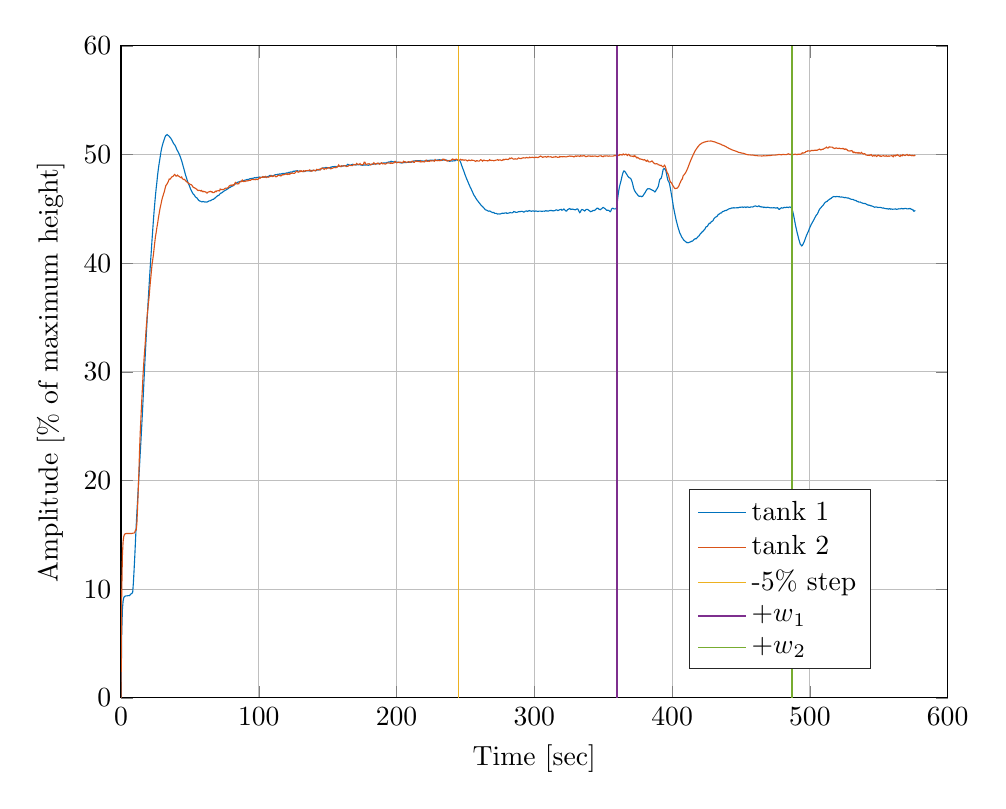
\begin{tikzpicture}

\begin{axis}[%
width=4.133in,
height=3.26in,
at={(0.693in,0.44in)},
scale only axis,
xmin=0,
xmax=600,
xlabel={Time [sec]},
xmajorgrids,
ymin=0,
ymax=60,
ymajorgrids,
ylabel={Amplitude [$\%$ of maximum height]},
axis background/.style={fill=white},
legend style={at={(0.687,0.044)},anchor=south west,legend cell align=left,align=left,draw=white!15!black}
]
\addplot [color=mycolor1,solid]
  table[row sep=crcr]{%
0	0\\
0.5	5.92896939554139\\
1	8.10860369066543\\
1.5	8.91339347310393\\
2	9.20976999001921\\
2.5	9.31816099244337\\
3	9.35747802609053\\
3.5	9.37383969335179\\
4	9.37915382890133\\
4.5	9.37956601254158\\
5	9.40327438110715\\
5.5	9.400570566791\\
6	9.39583980316239\\
6.5	9.45153122980255\\
7	9.53434653472947\\
7.5	9.57975515688143\\
8	9.61017162829475\\
8.5	9.73769273358039\\
9	10.6439771000273\\
9.5	11.8130004038294\\
10	13.0572924955113\\
10.5	14.4442919754043\\
11	15.8122983745749\\
11.5	17.017815115377\\
12	18.1295828391016\\
12.5	19.2386991100846\\
13	20.373388977876\\
13.5	21.484077703963\\
14	22.6515339829306\\
14.5	23.757827255241\\
15	24.9344134270708\\
15.5	26.1382621062854\\
16	27.4323531820333\\
16.5	28.7507189952972\\
17	30.0656441911842\\
17.5	31.3197166428647\\
18	32.5503840805675\\
18.5	33.7568725416367\\
19	34.9151408480436\\
19.5	36.0528244637622\\
20	37.1505237568931\\
20.5	38.2024158167699\\
21	39.2407091357341\\
21.5	40.2536540251136\\
22	41.1544636982189\\
22.5	42.1371852251679\\
23	43.0192667812315\\
23.5	43.9344548384687\\
24	44.7549957067438\\
24.5	45.5000246225729\\
25	46.2284749768755\\
25.5	46.8622464178779\\
26	47.4151869547427\\
26.5	48.0480422984717\\
27	48.5698199333064\\
27.5	49.0308093012963\\
28	49.4301903309538\\
28.5	49.8409253816763\\
29	50.2514772840452\\
29.5	50.5781202673724\\
30	50.838080505254\\
30.5	51.0506112028884\\
31	51.2350671643899\\
31.5	51.42665660448\\
32	51.6166562765112\\
32.5	51.7326152912065\\
33	51.7895468058724\\
33.5	51.8367696730281\\
34	51.7632554573314\\
34.5	51.7208260760919\\
35	51.6695495302774\\
35.5	51.5857977942409\\
36	51.5135315526247\\
36.5	51.4096101471888\\
37	51.3073884795288\\
37.5	51.1739319553661\\
38	51.0448043488468\\
38.5	50.9507738499009\\
39	50.8816300759237\\
39.5	50.7654239321492\\
40	50.6239200257142\\
40.5	50.4478171190263\\
41	50.3469464548943\\
41.5	50.2272559518934\\
42	50.1042378703674\\
42.5	49.9492398065189\\
43	49.800382632348\\
43.5	49.6086471291897\\
44	49.4163104637513\\
44.5	49.2097840356929\\
45	48.9588360414869\\
45.5	48.7358582763543\\
46	48.5204438887689\\
46.5	48.2597431006053\\
47	48.0469534553862\\
47.5	47.8573385196656\\
48	47.6487030152495\\
48.5	47.4565385731877\\
49	47.3005553852787\\
49.5	47.157076001721\\
50	46.9900361723172\\
50.5	46.8111807734486\\
51	46.6884042776827\\
51.5	46.5644112615883\\
52	46.4448070945128\\
52.5	46.3432200158334\\
53	46.2981560559008\\
53.5	46.2034286677675\\
54	46.0993952008138\\
54.5	46.0342426714687\\
55	46.0167298728204\\
55.5	45.9317398843104\\
56	45.8427811861369\\
56.5	45.7682871749678\\
57	45.7224424684711\\
57.5	45.7053468285071\\
58	45.6826245428621\\
58.5	45.6414568190428\\
59	45.6432581432611\\
59.5	45.6779425863807\\
60	45.656252515953\\
60.5	45.6295598303815\\
61	45.6398974025829\\
61.5	45.623176440783\\
62	45.6196836196478\\
62.5	45.6271208328823\\
63	45.654862077485\\
63.5	45.6883084452548\\
64	45.7353045339506\\
64.5	45.7281690722861\\
65	45.7518203103614\\
65.5	45.8025765277577\\
66	45.8186987024679\\
66.5	45.8680438865943\\
67	45.8665095715656\\
67.5	45.9179757141053\\
68	45.9668897947844\\
68.5	46.0272780550042\\
69	46.08451103421\\
69.5	46.1510434148835\\
70	46.1714572126407\\
70.5	46.2395365637793\\
71	46.2438756544735\\
71.5	46.3231047532168\\
72	46.3901124482106\\
72.5	46.4499789905113\\
73	46.4558770273192\\
73.5	46.5059962613998\\
74	46.5610143742067\\
74.5	46.6116222648773\\
75	46.6448247535764\\
75.5	46.6906696675384\\
76	46.726299254869\\
76.5	46.7522705142851\\
77	46.8075667527195\\
77.5	46.8463225940322\\
78	46.8776240527489\\
78.5	46.9355869039071\\
79	46.9585788273408\\
79.5	46.9868512644453\\
80	47.0589943643911\\
80.5	47.0630350414711\\
81	47.1115720915978\\
81.5	47.1243967538602\\
82	47.2133573890861\\
82.5	47.2593181480531\\
83	47.2868878223664\\
83.5	47.3421994090898\\
84	47.3810799373009\\
84.5	47.4344041931431\\
85	47.460812996032\\
85.5	47.4709231101114\\
86	47.4956612259332\\
86.5	47.5198312313727\\
87	47.5493911771581\\
87.5	47.5482920998956\\
88	47.5523373946714\\
88.5	47.5961892630383\\
89	47.5958240218596\\
89.5	47.6225181709344\\
90	47.6384376450056\\
90.5	47.6493350671432\\
91	47.6671907612699\\
91.5	47.710644006769\\
92	47.7098711545948\\
92.5	47.7034190517805\\
93	47.7347165421547\\
93.5	47.7643755071716\\
94	47.7826300828063\\
94.5	47.7844927636501\\
95	47.7916065987212\\
95.5	47.8036847733191\\
96	47.8166811802707\\
96.5	47.8435250116834\\
97	47.8712905276468\\
97.5	47.8511103523696\\
98	47.8532159289052\\
98.5	47.8869210538219\\
99	47.8838356600711\\
99.5	47.8844398111667\\
100	47.9065609749615\\
100.5	47.9237011510035\\
101	47.9084560569985\\
101.5	47.8908382444219\\
102	47.8926332981964\\
102.5	47.9093280727171\\
103	47.9311163900124\\
103.5	47.9312298020108\\
104	47.9435010763171\\
104.5	47.9086230081224\\
105	47.9110310666497\\
105.5	47.9128966987418\\
106	47.9519899899207\\
106.5	47.9680937896216\\
107	47.9769860377645\\
107.5	48.0209695766466\\
108	48.0693911423261\\
108.5	48.0626310742237\\
109	48.0568106728811\\
109.5	48.0312867536745\\
110	48.0352573789707\\
110.5	48.0459263442842\\
111	48.0743966199162\\
111.5	48.1112273362046\\
112	48.131383288559\\
112.5	48.1430422528869\\
113	48.1471682860548\\
113.5	48.1646970013622\\
114	48.1812043780217\\
114.5	48.1688225872182\\
115	48.2018597702534\\
115.5	48.2052124412121\\
116	48.1857456770979\\
116.5	48.2252200848887\\
117	48.2364855018742\\
117.5	48.2580010295526\\
118	48.2526573529219\\
118.5	48.2531984673736\\
119	48.2560068400248\\
119.5	48.2751964990907\\
120	48.2948120556639\\
120.5	48.2885089284806\\
121	48.2962184895747\\
121.5	48.344876249657\\
122	48.3428986072355\\
122.5	48.3565635548284\\
123	48.3849658227847\\
123.5	48.3855025781323\\
124	48.3791752804414\\
124.5	48.3845614600083\\
125	48.4603940333043\\
125.5	48.4591230615396\\
126	48.4512932215334\\
126.5	48.4881534871637\\
127	48.4820038743335\\
127.5	48.4860211494037\\
128	48.5101148275751\\
128.5	48.4725744543306\\
129	48.4669901948087\\
129.5	48.4748663473087\\
130	48.4707455119183\\
130.5	48.4462596928156\\
131	48.4458243852277\\
131.5	48.4486382429695\\
132	48.4330576309367\\
132.5	48.4176656408157\\
133	48.4282980322382\\
133.5	48.4481683568558\\
134	48.4697226343381\\
134.5	48.4973451316746\\
135	48.5059277999801\\
135.5	48.4924962556373\\
136	48.5050931905888\\
136.5	48.4875812277139\\
137	48.4775059340905\\
137.5	48.4706559976875\\
138	48.4929591209755\\
138.5	48.5339352373679\\
139	48.5307443795006\\
139.5	48.5299603223082\\
140	48.5175848802138\\
140.5	48.5128422897853\\
141	48.5319096757504\\
141.5	48.5204143212044\\
142	48.5522045204676\\
142.5	48.5726924252661\\
143	48.5855254050708\\
143.5	48.5688332787419\\
144	48.6468064668595\\
144.5	48.6226764505278\\
145	48.6277641022563\\
145.5	48.6979545414531\\
146	48.7002873276367\\
146.5	48.7666692809072\\
147	48.7703953637147\\
147.5	48.7588855114737\\
148	48.7624145171413\\
148.5	48.807486500161\\
149	48.7989545794348\\
149.5	48.793297844855\\
150	48.7937451156799\\
150.5	48.7582733281075\\
151	48.7809384137272\\
151.5	48.7784106073844\\
152	48.8269350562071\\
152.5	48.8234749445405\\
153	48.8592117600279\\
153.5	48.8813129741938\\
154	48.8725833631569\\
154.5	48.8646433368708\\
155	48.8937218593362\\
155.5	48.8580654329235\\
156	48.9052234526136\\
156.5	48.8727172201787\\
157	48.8739353298888\\
157.5	48.9218129626275\\
158	48.9328150240108\\
158.5	48.9019491633336\\
159	48.9203254563171\\
159.5	48.8988890982034\\
160	48.8845593679873\\
160.5	48.9295864316394\\
161	48.9506807454025\\
161.5	48.9665710782451\\
162	48.9611337274093\\
162.5	48.9747620000714\\
163	48.9756997624804\\
163.5	48.9704778600154\\
164	49.0220425291007\\
164.5	49.0905951174048\\
165	49.0741058426882\\
165.5	49.0367479626682\\
166	49.0239923080831\\
166.5	49.0125753980298\\
167	49.047202287195\\
167.5	49.0629562755445\\
168	49.0926448813924\\
168.5	49.062183703443\\
169	49.0711520400507\\
169.5	49.0476538002897\\
170	49.0598289327613\\
170.5	49.0343063995089\\
171	49.0407830121508\\
171.5	49.0574050798718\\
172	49.0722486500647\\
172.5	49.0539302334616\\
173	49.0790635899237\\
173.5	49.0550988977868\\
174	49.0316174083076\\
174.5	49.021577497507\\
175	49.0114092637101\\
175.5	49.0068703019648\\
176	49.0220499244395\\
176.5	49.0425079059608\\
177	49.0245650436346\\
177.5	49.026065897569\\
178	49.0544356750395\\
178.5	49.0220691720033\\
179	49.0216966444485\\
179.5	49.0032499401586\\
180	49.0246199035091\\
180.5	49.059880249803\\
181	49.0514738038172\\
181.5	49.0994003022836\\
182	49.0924266689036\\
182.5	49.0915798215559\\
183	49.0989546556816\\
183.5	49.1317864500501\\
184	49.1316112921306\\
184.5	49.1251018361544\\
185	49.1408112012786\\
185.5	49.1240329341953\\
186	49.1327658498679\\
186.5	49.1377132905465\\
187	49.1744467426744\\
187.5	49.1850387943314\\
188	49.1762191151673\\
188.5	49.1744233740703\\
189	49.2124014527182\\
189.5	49.1994605663354\\
190	49.1882912339446\\
190.5	49.227794860994\\
191	49.2130270567045\\
191.5	49.2234501830751\\
192	49.2217051384591\\
192.5	49.2105279469552\\
193	49.2604707305264\\
193.5	49.2651079491708\\
194	49.2951344006153\\
194.5	49.3175932284703\\
195	49.3014063969322\\
195.5	49.3289560078014\\
196	49.3771016378194\\
196.5	49.3473113885405\\
197	49.3358420893491\\
197.5	49.3185495351556\\
198	49.3261324806122\\
198.5	49.3534302880295\\
199	49.307581934045\\
199.5	49.3163796635398\\
200	49.2934379927687\\
200.5	49.2857779788765\\
201	49.2846430805794\\
201.5	49.2754870066816\\
202	49.2618792493745\\
202.5	49.2504358022615\\
203	49.2301567643651\\
203.5	49.2158954690359\\
204	49.2279936082349\\
204.5	49.2557413274365\\
205	49.2635166705039\\
205.5	49.2623573795823\\
206	49.2678431298513\\
206.5	49.2504575891115\\
207	49.2475898771258\\
207.5	49.2679835748642\\
208	49.2784502777015\\
208.5	49.2790936245084\\
209	49.280867491409\\
209.5	49.2822357181785\\
210	49.3039823932651\\
210.5	49.3055253423181\\
211	49.2893364568771\\
211.5	49.3276371304963\\
212	49.3599223957321\\
212.5	49.4025380533015\\
213	49.4084279639354\\
213.5	49.4122228692009\\
214	49.4363653540124\\
214.5	49.4324118694812\\
215	49.4384003652586\\
215.5	49.4258315305923\\
216	49.4279979026337\\
216.5	49.4314460213249\\
217	49.4228130801118\\
217.5	49.4274754024469\\
218	49.4087626409156\\
218.5	49.4039981879606\\
219	49.3975486911969\\
219.5	49.386720689147\\
220	49.4088372524782\\
220.5	49.3897663905028\\
221	49.4049917668562\\
221.5	49.4102340630597\\
222	49.4391856922723\\
222.5	49.4507820353566\\
223	49.4497890140608\\
223.5	49.4502985813251\\
224	49.4645703815421\\
224.5	49.4745990868209\\
225	49.4664248379617\\
225.5	49.4658839370776\\
226	49.4844807549991\\
226.5	49.482369332082\\
227	49.4445280022806\\
227.5	49.4701088174272\\
228	49.4740472329268\\
228.5	49.4480430642324\\
229	49.4717101064638\\
229.5	49.4994171285895\\
230	49.4889973707929\\
230.5	49.4930746670514\\
231	49.5153647675462\\
231.5	49.5103212863466\\
232	49.4951591473671\\
232.5	49.5040346575026\\
233	49.501043274742\\
233.5	49.4687956294244\\
234	49.5118081034603\\
234.5	49.4884442361548\\
235	49.4795598731329\\
235.5	49.4816660402119\\
236	49.4933173994587\\
236.5	49.4609466120672\\
237	49.451547923097\\
237.5	49.4238396215681\\
238	49.4041642974388\\
238.5	49.3678973803058\\
239	49.3900077317553\\
239.5	49.4067669329081\\
240	49.4047208073156\\
240.5	49.3957610624721\\
241	49.4111868665945\\
241.5	49.4134518756621\\
242	49.4247270546114\\
242.5	49.4170597982163\\
243	49.4883361799658\\
243.5	49.5012382264574\\
244	49.4919490215071\\
244.5	49.4541577480473\\
245	49.4345434139945\\
245.5	49.463107069398\\
246	49.4107397797129\\
246.5	49.2846246571578\\
247	49.1018015318424\\
247.5	48.9141231925217\\
248	48.7399042098785\\
248.5	48.5699227498152\\
249	48.4095708544855\\
249.5	48.2096400332372\\
250	48.0476622125915\\
250.5	47.8780663916555\\
251	47.7240886858723\\
251.5	47.5799727534906\\
252	47.4280125363318\\
252.5	47.2706405035433\\
253	47.1378485525735\\
253.5	46.9785741154669\\
254	46.8618378978519\\
254.5	46.7224640323589\\
255	46.5856670062807\\
255.5	46.4447732139617\\
256	46.289330156741\\
256.5	46.2015600604397\\
257	46.1074338724574\\
257.5	45.9828198925287\\
258	45.8858123437337\\
258.5	45.7964991032232\\
259	45.7195290017326\\
259.5	45.6249632729667\\
260	45.554958185713\\
260.5	45.4679861950117\\
261	45.386096283691\\
261.5	45.3085722998478\\
262	45.2534784743546\\
262.5	45.1995656310025\\
263	45.1193077856639\\
263.5	45.0571206266552\\
264	44.9817531205291\\
264.5	44.9135600789533\\
265	44.888774261986\\
265.5	44.8768771070719\\
266	44.8215044694694\\
266.5	44.7928223668096\\
267	44.7737189838144\\
267.5	44.7955070097366\\
268	44.7886673936182\\
268.5	44.7288764428066\\
269	44.701378614447\\
269.5	44.6512564022228\\
270	44.6730300871312\\
270.5	44.6662969133531\\
271	44.6000240725423\\
271.5	44.5791388809555\\
272	44.5795157666382\\
272.5	44.5755216463866\\
273	44.5290758828706\\
273.5	44.5166028166992\\
274	44.5284274778137\\
274.5	44.5369417320136\\
275	44.5163519005675\\
275.5	44.5334973261996\\
276	44.5670695620189\\
276.5	44.5865867240017\\
277	44.594233745504\\
277.5	44.5823002050379\\
278	44.5883442882816\\
278.5	44.6107312313193\\
279	44.6219296738116\\
279.5	44.6316166562411\\
280	44.5887622133514\\
280.5	44.5793528911173\\
281	44.602789375303\\
281.5	44.6120824042346\\
282	44.6288632141877\\
282.5	44.6619422113986\\
283	44.630975930734\\
283.5	44.6257535440572\\
284	44.6281985602538\\
284.5	44.6665566261938\\
285	44.7419762796565\\
285.5	44.724617113019\\
286	44.7215052801689\\
286.5	44.6709171477122\\
287	44.6675854342574\\
287.5	44.6814303082911\\
288	44.7064090794853\\
288.5	44.7320283523467\\
289	44.7478104091152\\
289.5	44.7283506076838\\
290	44.7452987348465\\
290.5	44.7691589038363\\
291	44.7701944537007\\
291.5	44.7566865158251\\
292	44.7097328810916\\
292.5	44.7002314773958\\
293	44.7374438835578\\
293.5	44.7874039284164\\
294	44.7951628141159\\
294.5	44.8011922328169\\
295	44.7576105561834\\
295.5	44.7835376152568\\
296	44.8160709603751\\
296.5	44.8371193644167\\
297	44.7893314421381\\
297.5	44.7945245681765\\
298	44.7723501372059\\
298.5	44.7971772832947\\
299	44.8083961921682\\
299.5	44.7940571402009\\
300	44.7764650142821\\
300.5	44.7788698680379\\
301	44.8051076661711\\
301.5	44.7876893967451\\
302	44.7774803770176\\
302.5	44.7511968168367\\
303	44.7665077699502\\
303.5	44.7881226706001\\
304	44.7893834457748\\
304.5	44.782950004943\\
305	44.7772476221521\\
305.5	44.7569412412219\\
306	44.7762063441198\\
306.5	44.783779982894\\
307	44.7880324009725\\
307.5	44.7759569972705\\
308	44.8151538086182\\
308.5	44.829099281315\\
309	44.7907155871939\\
309.5	44.8093951517948\\
310	44.7858105400889\\
310.5	44.8001234947877\\
311	44.8399141640671\\
311.5	44.836029999348\\
312	44.8534640135258\\
312.5	44.8430786095875\\
313	44.811582958428\\
313.5	44.8300289982793\\
314	44.8034196971272\\
314.5	44.8258920110495\\
315	44.8416410878431\\
315.5	44.8838593746327\\
316	44.9068450439114\\
316.5	44.8865452221936\\
317	44.8388341067351\\
317.5	44.8523779660501\\
318	44.8902974802315\\
318.5	44.9273800472767\\
319	44.9322353210612\\
319.5	44.9532871654078\\
320	44.8753450098992\\
320.5	44.8903489863645\\
321	44.9225188112728\\
321.5	44.981958767283\\
322	44.9096386446461\\
322.5	44.850799629926\\
323	44.7971577057227\\
323.5	44.7960937991598\\
324	44.9131449587545\\
324.5	44.9511765675427\\
325	44.9733737633763\\
325.5	45.0222968570234\\
326	44.9949117041892\\
326.5	44.9392074554107\\
327	44.9657868274369\\
327.5	44.9554706314477\\
328	44.9749637118423\\
328.5	44.9427934419954\\
329	44.9277189007267\\
329.5	44.9111490693312\\
330	44.9167263507964\\
330.5	44.960603697968\\
331	44.986928440375\\
331.5	44.9862679111843\\
332	44.8805128359207\\
332.5	44.7338391381995\\
333	44.6467682110625\\
333.5	44.7192745243249\\
334	44.8679565925719\\
334.5	44.939139323186\\
335	44.9140301081634\\
335.5	44.8996004905188\\
336	44.854915483579\\
336.5	44.8033021689352\\
337	44.841330918888\\
337.5	44.934740658768\\
338	44.9520636320562\\
338.5	44.9419477297955\\
339	44.9239716656231\\
339.5	44.8624286211527\\
340	44.8168715799269\\
340.5	44.7666646495254\\
341	44.7333873540482\\
341.5	44.7694558912901\\
342	44.7796227312938\\
342.5	44.8422414423632\\
343	44.843244678172\\
343.5	44.8404027801157\\
344	44.8756007962169\\
344.5	44.953947370817\\
345	44.9828642253417\\
345.5	45.0555934046197\\
346	45.0507541369985\\
346.5	45.0338402892744\\
347	44.9426722926661\\
347.5	44.9371829318395\\
348	44.9150698334479\\
348.5	44.9763666274016\\
349	45.0223770325694\\
349.5	45.0922021877759\\
350	45.1254096927789\\
350.5	45.086478953178\\
351	45.0450671258639\\
351.5	44.9985250428735\\
352	44.9301081268094\\
352.5	44.869889931023\\
353	44.8650245743184\\
353.5	44.8669280517212\\
354	44.852772457937\\
354.5	44.7917711693741\\
355	44.7287973369089\\
355.5	44.7881249380863\\
356	44.9602220721227\\
356.5	45.0374683726979\\
357	45.0583387450096\\
357.5	45.0039409746287\\
358	44.9933045932635\\
358.5	44.9867416100494\\
359	44.9996119176086\\
359.5	44.9830053864428\\
360	45.357962030846\\
360.5	45.9172891596149\\
361	46.4354647893772\\
361.5	46.8336957532409\\
362	47.1385295083045\\
362.5	47.3824159034037\\
363	47.6190169883252\\
363.5	47.9097241073466\\
364	48.166851217442\\
364.5	48.3763306017243\\
365	48.4843797250814\\
365.5	48.4600840805842\\
366	48.3845034831547\\
366.5	48.2871673812536\\
367	48.1979619517\\
367.5	48.0772693601892\\
368	47.9795999798895\\
368.5	47.9097550782027\\
369	47.8481425029081\\
369.5	47.8241821249431\\
370	47.7809325914236\\
370.5	47.6374430591988\\
371	47.4738241308274\\
371.5	47.2265527109444\\
372	46.9444130357179\\
372.5	46.7442042576347\\
373	46.6309867788326\\
373.5	46.5138983042969\\
374	46.4416280474774\\
374.5	46.3642153721923\\
375	46.2770881952673\\
375.5	46.2117760994172\\
376	46.1565866319178\\
376.5	46.1528634413829\\
377	46.1663278771805\\
377.5	46.1471475112397\\
378	46.1139197291735\\
378.5	46.1488234213054\\
379	46.2169844556543\\
379.5	46.3260195960392\\
380	46.4253649480934\\
380.5	46.502111435399\\
381	46.6360331455944\\
381.5	46.7308628156444\\
382	46.8121211883627\\
382.5	46.8505797160316\\
383	46.8353047192369\\
383.5	46.8423296284039\\
384	46.8328305253007\\
384.5	46.783009489756\\
385	46.7594619239225\\
385.5	46.7171335128537\\
386	46.6994312568843\\
386.5	46.6665039715207\\
387	46.6080635419464\\
387.5	46.556462936446\\
388	46.6113039402702\\
388.5	46.7525139800974\\
389	46.8277055920219\\
389.5	46.9607046197841\\
390	47.076645218872\\
390.5	47.3869182188748\\
391	47.6791654183623\\
391.5	47.7697225100621\\
392	47.8022574485982\\
392.5	47.9929660173795\\
393	48.2985919130754\\
393.5	48.6199366596675\\
394	48.6837852234697\\
394.5	48.6855779333927\\
395	48.6098297492978\\
395.5	48.4968215073397\\
396	48.1815153783283\\
396.5	47.8744338521081\\
397	47.5960421227612\\
397.5	47.5153480980496\\
398	47.365432095288\\
398.5	47.068895110302\\
399	46.695239043761\\
399.5	46.3376751292508\\
400	45.9664499044129\\
400.5	45.5697816115576\\
401	45.1559755409715\\
401.5	44.8419373769369\\
402	44.5190375810154\\
402.5	44.2272707429466\\
403	43.9274091666265\\
403.5	43.68220232703\\
404	43.4312391574222\\
404.5	43.214931314774\\
405	43.0117201319414\\
405.5	42.8094446102323\\
406	42.664613999122\\
406.5	42.5387951470958\\
407	42.3945600438829\\
407.5	42.3132511464485\\
408	42.2146594350658\\
408.5	42.1190615198777\\
409	42.0664267967113\\
409.5	42.0009899198102\\
410	41.9642115023989\\
410.5	41.8910553080912\\
411	41.9003846453442\\
411.5	41.8738105496742\\
412	41.8917375292409\\
412.5	41.9181819806517\\
413	41.9441976788627\\
413.5	41.9634937693506\\
414	42.0142367655031\\
414.5	42.019237919552\\
415	42.041169216474\\
415.5	42.1198784395562\\
416	42.1861173535639\\
416.5	42.2126499029823\\
417	42.2638368065191\\
417.5	42.244769077199\\
418	42.322194955614\\
418.5	42.3799587655421\\
419	42.4664462649803\\
419.5	42.4973135173327\\
420	42.5930811897487\\
420.5	42.6993993097692\\
421	42.7515865813205\\
421.5	42.8437386497181\\
422	42.8781155342006\\
422.5	42.9410876545512\\
423	43.0314443047982\\
423.5	43.0776289359723\\
424	43.176700789743\\
424.5	43.3212579274726\\
425	43.3530057557237\\
425.5	43.3758105013139\\
426	43.4756157940976\\
426.5	43.5824314637979\\
427	43.6704886552349\\
427.5	43.6540999439106\\
428	43.7243482099991\\
428.5	43.8148663143934\\
429	43.8473332177251\\
429.5	43.8803152724137\\
430	43.9876830989933\\
430.5	44.1127053284873\\
431	44.1765638170423\\
431.5	44.2300612951547\\
432	44.2629656593434\\
432.5	44.3060377321046\\
433	44.3571978963166\\
433.5	44.4797858523653\\
434	44.4959022219926\\
434.5	44.553228217563\\
435	44.6096908811052\\
435.5	44.6009069674688\\
436	44.6488201541857\\
436.5	44.7350059802841\\
437	44.7549384707281\\
437.5	44.7704727507523\\
438	44.8174041169826\\
438.5	44.8393248667936\\
439	44.8417721888453\\
439.5	44.8524470653674\\
440	44.9054466720948\\
440.5	44.9395524514924\\
441	44.9776538608151\\
441.5	45.0053295163252\\
442	45.0219612747006\\
442.5	45.0302472162147\\
443	45.0591446841184\\
443.5	45.0880338665755\\
444	45.069672942775\\
444.5	45.0961134168555\\
445	45.0712031823619\\
445.5	45.0926974228012\\
446	45.0845041842665\\
446.5	45.0864103622237\\
447	45.1027798948314\\
447.5	45.0952069256572\\
448	45.0933489381814\\
448.5	45.1267854710893\\
449	45.1407579312804\\
449.5	45.1442696233009\\
450	45.1439011036333\\
450.5	45.1572623608953\\
451	45.1741658338152\\
451.5	45.1267966946973\\
452	45.1460549409134\\
452.5	45.1616415084624\\
453	45.1691505947937\\
453.5	45.1209472000351\\
454	45.1522081018381\\
454.5	45.1771064821261\\
455	45.1649109483775\\
455.5	45.1409196854449\\
456	45.1367570091361\\
456.5	45.128138836215\\
457	45.1624795903332\\
457.5	45.1770528759089\\
458	45.1764354415171\\
458.5	45.1675657361111\\
459	45.1924444447667\\
459.5	45.2301569381639\\
460	45.251482965771\\
460.5	45.2592305844788\\
461	45.2476468089755\\
461.5	45.2214584026792\\
462	45.2015547798252\\
462.5	45.2323873463556\\
463	45.2679403612225\\
463.5	45.210604151728\\
464	45.1792223493973\\
464.5	45.2060946414014\\
465	45.1596281494543\\
465.5	45.1591270810775\\
466	45.1762561653484\\
466.5	45.1121739411744\\
467	45.1403568018152\\
467.5	45.1382556522829\\
468	45.1086719590836\\
468.5	45.1153725629814\\
469	45.1542773187758\\
469.5	45.1310798003106\\
470	45.137797187179\\
470.5	45.1096655143257\\
471	45.0960783406094\\
471.5	45.0864112329018\\
472	45.0970201109287\\
472.5	45.0876588363189\\
473	45.0916014755365\\
473.5	45.093149995215\\
474	45.1044320320139\\
474.5	45.0838004371991\\
475	45.0743614279327\\
475.5	45.0671698334126\\
476	45.0882912863789\\
476.5	45.1052907422286\\
477	45.0321389083086\\
477.5	44.959271658496\\
478	44.9615198787597\\
478.5	45.0310969214849\\
479	45.0618453974096\\
479.5	45.0996985265014\\
480	45.0692608972251\\
480.5	45.0660413791328\\
481	45.1174166918757\\
481.5	45.1385448597939\\
482	45.1142171621635\\
482.5	45.1107050857134\\
483	45.1445439120786\\
483.5	45.1317064473139\\
484	45.1499843287478\\
484.5	45.1165032559898\\
485	45.1532311630642\\
485.5	45.1773079863873\\
486	45.1368814119648\\
486.5	45.097156070648\\
487	44.9582527898539\\
487.5	44.7942051175951\\
488	44.5264671577309\\
488.5	44.2197140730407\\
489	43.8777514553463\\
489.5	43.5355624763356\\
490	43.2398423191354\\
490.5	42.9512452432114\\
491	42.69457055922\\
491.5	42.4445165594991\\
492	42.1817317104014\\
492.5	41.9786732713976\\
493	41.7584432623026\\
493.5	41.6897365864094\\
494	41.5829184686302\\
494.5	41.6177024371152\\
495	41.7304043253423\\
495.5	41.8815807501527\\
496	42.0035178281114\\
496.5	42.1862832933424\\
497	42.3626106380239\\
497.5	42.532089585998\\
498	42.6731486367475\\
498.5	42.8154064018668\\
499	42.9409898744845\\
499.5	43.1370315802319\\
500	43.2767324785443\\
500.5	43.4157704866419\\
501	43.5641308139297\\
501.5	43.6693979045196\\
502	43.787408543017\\
502.5	43.8995622654672\\
503	44.0106440749519\\
503.5	44.1482382484629\\
504	44.2606557275693\\
504.5	44.3733094222211\\
505	44.4691336999621\\
505.5	44.5343546440288\\
506	44.6709364280628\\
506.5	44.8214898174278\\
507	44.9390301144651\\
507.5	45.0327531184668\\
508	45.0947146120988\\
508.5	45.1829610114277\\
509	45.2417798342133\\
509.5	45.3067854079055\\
510	45.3947791661497\\
510.5	45.4920927371987\\
511	45.5781574277197\\
511.5	45.6171568334739\\
512	45.6658744144564\\
512.5	45.6768456167605\\
513	45.7529391052704\\
513.5	45.8081865202634\\
514	45.849219505594\\
514.5	45.8883381546744\\
515	45.9475912315489\\
515.5	45.9682479488191\\
516	46.0357460796802\\
516.5	46.0722697803852\\
517	46.1173743798799\\
517.5	46.1314494427301\\
518	46.1157783114373\\
518.5	46.1116861233119\\
519	46.1142347076483\\
519.5	46.1378958847625\\
520	46.1253778375499\\
520.5	46.1231437666976\\
521	46.1084930858558\\
521.5	46.1260232000542\\
522	46.0746699708869\\
522.5	46.0794266816338\\
523	46.0843252646085\\
523.5	46.0813191759858\\
524	46.0677035203451\\
524.5	46.0546569779917\\
525	46.0226647550321\\
525.5	46.0352691068004\\
526	46.0416251896997\\
526.5	46.0079875612895\\
527	46.0021994813831\\
527.5	45.9901788106829\\
528	45.9952468299542\\
528.5	45.9605619695044\\
529	45.9249191778279\\
529.5	45.9041128557212\\
530	45.8728731511739\\
530.5	45.8698403528123\\
531	45.8691826682955\\
531.5	45.8528116130248\\
532	45.8103879455563\\
532.5	45.793212461289\\
533	45.7579877879483\\
533.5	45.7611397291687\\
534	45.7179637097319\\
534.5	45.6594148617307\\
535	45.6696346747011\\
535.5	45.6173881903318\\
536	45.6120972590854\\
536.5	45.6248301425041\\
537	45.5880009928547\\
537.5	45.5453475599324\\
538	45.5415557096524\\
538.5	45.5108123028191\\
539	45.4942431203214\\
539.5	45.4781697262479\\
540	45.4975174309527\\
540.5	45.4673900849991\\
541	45.4240579273507\\
541.5	45.3927054427682\\
542	45.3542465465575\\
542.5	45.3507797023318\\
543	45.3160931872265\\
543.5	45.3267665454084\\
544	45.2697180132234\\
544.5	45.2810930234311\\
545	45.246692650973\\
545.5	45.2361931927065\\
546	45.2038019634506\\
546.5	45.1787441693656\\
547	45.1459411976378\\
547.5	45.15015533847\\
548	45.1774756126556\\
548.5	45.1554126832718\\
549	45.1453867620789\\
549.5	45.1158282444668\\
550	45.1350688053809\\
550.5	45.1254048373638\\
551	45.1358505948349\\
551.5	45.1151102819552\\
552	45.0986572282917\\
552.5	45.0803251632016\\
553	45.0622067234355\\
553.5	45.0781007604929\\
554	45.0466631204563\\
554.5	45.0324293905706\\
555	45.0140868225984\\
555.5	45.0166324990398\\
556	44.9912567723421\\
556.5	45.0056824445905\\
557	44.9679555835322\\
557.5	45.0058551080795\\
558	45.0081386040063\\
558.5	44.9652471083062\\
559	44.9869636163669\\
559.5	44.9685576107991\\
560	44.9598666406757\\
560.5	44.9653895456881\\
561	44.9677444780071\\
561.5	44.9752804141135\\
562	44.9976236370495\\
562.5	44.9678153317304\\
563	44.9495192270272\\
563.5	44.9634976756295\\
564	44.9824264705061\\
564.5	45.0036050994699\\
565	44.9935555595467\\
565.5	44.9943290061003\\
566	45.0083332306791\\
566.5	45.0367277518473\\
567	44.9996984313514\\
567.5	45.0121777252147\\
568	45.0002050362615\\
568.5	45.015826738978\\
569	45.035234466514\\
569.5	45.0333092711045\\
570	45.0232243566455\\
570.5	44.9934327035911\\
571	44.9980552544414\\
571.5	45.0049039724534\\
572	45.0057911752448\\
572.5	45.0321575162739\\
573	45.0225587316506\\
573.5	44.958896277944\\
574	44.955642907892\\
574.5	44.8963862120463\\
575	44.8890690880751\\
575.5	44.7732234068613\\
576	44.7967649295352\\
576.5	44.8514831363771\\
};
\addlegendentry{tank 1};

\addplot [color=mycolor2,solid]
  table[row sep=crcr]{%
0	0\\
0.5	9.55825510605771\\
1	13.0756081161211\\
1.5	14.371873397059\\
2	14.8509326040342\\
2.5	15.0261022317412\\
3	15.0901801721311\\
3.5	15.1110187689332\\
4	15.1190215722158\\
4.5	15.1227358484718\\
5	15.1227655893828\\
5.5	15.1209705574686\\
6	15.1169512992508\\
6.5	15.1178899033118\\
7	15.1158246552924\\
7.5	15.1136340118525\\
8	15.1325742972995\\
8.5	15.1451672676613\\
9	15.1550791616819\\
9.5	15.1590604376356\\
10	15.2423347820809\\
10.5	15.4192458778677\\
11	15.4467198280626\\
11.5	16.0116238739013\\
12	17.4608977928324\\
12.5	19.1331732262795\\
13	20.9036919777727\\
13.5	22.9618966423638\\
14	24.5801041687517\\
14.5	25.882673614569\\
15	27.2524525569571\\
15.5	28.4061165143335\\
16	29.7440264887432\\
16.5	30.7902772383479\\
17	31.696191060494\\
17.5	32.5137522222798\\
18	33.5252614722378\\
18.5	34.3822154208811\\
19	35.1754975392299\\
19.5	35.8167971580459\\
20	36.4126983791518\\
20.5	37.054225622759\\
21	37.8588590981427\\
21.5	38.5334717339934\\
22	39.1829769953475\\
22.5	39.8558007564719\\
23	40.2994347628165\\
23.5	40.7774149005565\\
24	41.3342609851844\\
24.5	41.9034845147215\\
25	42.4480042461737\\
25.5	42.8085489983353\\
26	43.255807167732\\
26.5	43.6083444871465\\
27	44.0469040895414\\
27.5	44.4320485982061\\
28	44.8141276278517\\
28.5	45.1498823466101\\
29	45.4231880622423\\
29.5	45.7402375551738\\
30	46.0049396304125\\
30.5	46.2051335746717\\
31	46.4124548149625\\
31.5	46.6010026097707\\
32	46.8905144110962\\
32.5	47.1143307217039\\
33	47.2267028855458\\
33.5	47.3030377900473\\
34	47.4194308284737\\
34.5	47.5702527930512\\
35	47.7426875908221\\
35.5	47.7232696226788\\
36	47.7696801414137\\
36.5	47.8899519169218\\
37	47.9419540451269\\
37.5	47.9715694833265\\
38	48.0229921829365\\
38.5	48.1024672712559\\
39	48.1649128490768\\
39.5	48.0729192601287\\
40	48.0080698026882\\
40.5	48.0083717426704\\
41	48.0988964578227\\
41.5	48.028824658548\\
42	47.9967277155135\\
42.5	47.9603391405649\\
43	47.8946798446793\\
43.5	47.8648673495294\\
44	47.9301163335587\\
44.5	47.7928578013282\\
45	47.7200655217862\\
45.5	47.6941209284313\\
46	47.7112334970515\\
46.5	47.6477324314628\\
47	47.5489750236432\\
47.5	47.5424292803403\\
48	47.4401297353802\\
48.5	47.4094620777015\\
49	47.3425107249475\\
49.5	47.3004597252135\\
50	47.2657021694205\\
50.5	47.223945098092\\
51	47.217696983046\\
51.5	47.1523425378625\\
52	47.0595587326829\\
52.5	46.9670392966312\\
53	46.941135141091\\
53.5	46.9314149673337\\
54	46.8736414719252\\
54.5	46.8348807529027\\
55	46.8035603587862\\
55.5	46.7090323557129\\
56	46.6771548511841\\
56.5	46.7056756463011\\
57	46.6980010919011\\
57.5	46.6673718655353\\
58	46.6391283350443\\
58.5	46.6907295020689\\
59	46.6036413878432\\
59.5	46.5645961349991\\
60	46.609526140621\\
60.5	46.5829139322217\\
61	46.5628001403475\\
61.5	46.5529581914788\\
62	46.4707699385082\\
62.5	46.4461187244869\\
63	46.520844658752\\
63.5	46.5561118939827\\
64	46.5551161549365\\
64.5	46.593498223053\\
65	46.6095924655092\\
65.5	46.5504608527373\\
66	46.576376106935\\
66.5	46.5004378088766\\
67	46.492553536338\\
67.5	46.4963877335854\\
68	46.5514964448849\\
68.5	46.6181212060225\\
69	46.5724236733813\\
69.5	46.6533976849219\\
70	46.6488845403068\\
70.5	46.6786664346311\\
71	46.6584716936497\\
71.5	46.6473325508009\\
72	46.8197353041418\\
72.5	46.7668535739395\\
73	46.7775329444668\\
73.5	46.7757275585768\\
74	46.7555106699257\\
74.5	46.7825450680291\\
75	46.8281363733751\\
75.5	46.8832965068856\\
76	46.9055769750408\\
76.5	46.8936960028794\\
77	46.908845484514\\
77.5	46.9285813556406\\
78	46.9764738758134\\
78.5	47.101144734494\\
79	47.1372572013949\\
79.5	47.1775797344731\\
80	47.1879444987564\\
80.5	47.1197793192182\\
81	47.1932270823228\\
81.5	47.2167761191039\\
82	47.1709176121711\\
82.5	47.3111468925645\\
83	47.4309817717484\\
83.5	47.3944365970666\\
84	47.2989174554124\\
84.5	47.2858631625889\\
85	47.3091060132511\\
85.5	47.3070658359085\\
86	47.4546746159617\\
86.5	47.4734642263538\\
87	47.4754474687717\\
87.5	47.5441541308132\\
88	47.6418359766169\\
88.5	47.5178391018107\\
89	47.5158842032467\\
89.5	47.5471135632094\\
90	47.5098922432928\\
90.5	47.5577900836152\\
91	47.5691286741961\\
91.5	47.5558270462559\\
92	47.5983255410594\\
92.5	47.5846028180182\\
93	47.6148294859437\\
93.5	47.6249424474532\\
94	47.6291133130257\\
94.5	47.6826000145084\\
95	47.7146419863318\\
95.5	47.7031173417685\\
96	47.6815352633064\\
96.5	47.6973918620524\\
97	47.6865590182\\
97.5	47.6800007517763\\
98	47.7331144240572\\
98.5	47.7076084859494\\
99	47.6931628748299\\
99.5	47.7121454179388\\
100	47.8133981963769\\
100.5	47.8686153037298\\
101	47.817663634047\\
101.5	47.8825979785669\\
102	47.8949290675559\\
102.5	47.9016439200412\\
103	47.967523711836\\
103.5	47.9056686197592\\
104	47.9048922543493\\
104.5	47.9585918984649\\
105	47.985803612114\\
105.5	47.8760896302077\\
106	47.9108304581806\\
106.5	47.9172647038638\\
107	47.9096009851378\\
107.5	47.9368312573983\\
108	47.9610359182706\\
108.5	47.9863514722244\\
109	48.0569141748989\\
109.5	47.9781597088012\\
110	47.9696227261494\\
110.5	47.9816996629268\\
111	48.0420516697196\\
111.5	48.0759985617653\\
112	47.9804716289863\\
112.5	47.9419725806904\\
113	47.9840557701167\\
113.5	48.0061351007943\\
114	48.0855454714107\\
114.5	48.0956967529179\\
115	48.0660648850663\\
115.5	48.0628014452858\\
116	48.0250853024228\\
116.5	48.0465274929877\\
117	48.138750003336\\
117.5	48.1362967757484\\
118	48.1348546017206\\
118.5	48.1447890962893\\
119	48.1694501420268\\
119.5	48.2070928018259\\
120	48.1800586500274\\
120.5	48.2281963590423\\
121	48.159489693923\\
121.5	48.1817611629492\\
122	48.2250659257225\\
122.5	48.1660190346998\\
123	48.2598378875288\\
123.5	48.2876785738285\\
124	48.2666598627872\\
124.5	48.2945103450048\\
125	48.268120431829\\
125.5	48.2610753302464\\
126	48.2677859033351\\
126.5	48.3275224114974\\
127	48.4060103768506\\
127.5	48.4741590817111\\
128	48.4305072316305\\
128.5	48.3644150138193\\
129	48.3731431102549\\
129.5	48.4191622641643\\
130	48.503624753341\\
130.5	48.4317402502394\\
131	48.4903985749137\\
131.5	48.435411442732\\
132	48.4203732307869\\
132.5	48.5086084092329\\
133	48.4771659151028\\
133.5	48.4499270736824\\
134	48.5188309745415\\
134.5	48.5183545947601\\
135	48.5085766308511\\
135.5	48.5191997800233\\
136	48.5274086828294\\
136.5	48.5300238227179\\
137	48.5898758761739\\
137.5	48.5053825584\\
138	48.4585972639264\\
138.5	48.4855426056569\\
139	48.4837184849161\\
139.5	48.5590062980737\\
140	48.5680133688711\\
140.5	48.5226410761208\\
141	48.4877225127447\\
141.5	48.5226168077445\\
142	48.6321526277665\\
142.5	48.6103747502418\\
143	48.5870259299919\\
143.5	48.6176194224659\\
144	48.5894269386545\\
144.5	48.5647516785902\\
145	48.6733896856323\\
145.5	48.7342209207614\\
146	48.7299020714174\\
146.5	48.7501727731668\\
147	48.6756708529832\\
147.5	48.6320184852368\\
148	48.6942668876508\\
148.5	48.728892575063\\
149	48.6703679820924\\
149.5	48.7140598441615\\
150	48.75973855382\\
150.5	48.784589766093\\
151	48.7791499380682\\
151.5	48.7455777841571\\
152	48.6879284225522\\
152.5	48.6881952135324\\
153	48.7357261801881\\
153.5	48.7330746953471\\
154	48.7637825890621\\
154.5	48.7954783952051\\
155	48.7901681472151\\
155.5	48.8026316506814\\
156	48.7750700935662\\
156.5	48.8609352224035\\
157	48.8507924285403\\
157.5	48.9170787921816\\
158	49.0349799112812\\
158.5	48.9198336945016\\
159	48.8920055217083\\
159.5	48.883737363619\\
160	48.9626153653483\\
160.5	48.929935331086\\
161	48.9230548113509\\
161.5	48.9451730979868\\
162	48.9790226617876\\
162.5	48.9606815104985\\
163	48.9531656897519\\
163.5	48.89082561913\\
164	48.9083678299534\\
164.5	48.9090975448822\\
165	48.948246745418\\
165.5	48.9959503823651\\
166	49.0175233490126\\
166.5	48.9900349864713\\
167	48.9754323361168\\
167.5	48.9968230340171\\
168	48.9837302209249\\
168.5	49.0380976323579\\
169	49.0885106616071\\
169.5	49.0680924486045\\
170	49.04118288324\\
170.5	49.0481650669595\\
171	49.1700323940117\\
171.5	49.1232657961846\\
172	49.1076727642552\\
172.5	49.0717526973504\\
173	49.0846561995486\\
173.5	49.1601485345045\\
174	49.0842041460956\\
174.5	49.0708205295746\\
175	49.0445358183626\\
175.5	49.059979701816\\
176	49.1097561830175\\
176.5	49.2938174672507\\
177	49.2923319589241\\
177.5	49.134881878322\\
178	49.0587567606436\\
178.5	49.1013220124486\\
179	49.1375750050957\\
179.5	49.1286153891087\\
180	49.146734098358\\
180.5	49.1217853919458\\
181	49.0502867428291\\
181.5	49.0515956220123\\
182	49.0973907932796\\
182.5	49.1277956499053\\
183	49.1449455340752\\
183.5	49.2357025017004\\
184	49.1631828120423\\
184.5	49.0861501005311\\
185	49.1387368471675\\
185.5	49.1712874489401\\
186	49.1587094385334\\
186.5	49.2130889162297\\
187	49.1813591647975\\
187.5	49.0936958592676\\
188	49.1220344301571\\
188.5	49.1565010525069\\
189	49.2406082149768\\
189.5	49.205235135648\\
190	49.1271014814505\\
190.5	49.1555921622057\\
191	49.1623874583286\\
191.5	49.1255192758863\\
192	49.121421561957\\
192.5	49.154785652973\\
193	49.2061756170726\\
193.5	49.2216836660653\\
194	49.2278528740536\\
194.5	49.207536362566\\
195	49.2064896743474\\
195.5	49.1800445132754\\
196	49.2475340047551\\
196.5	49.1888136879921\\
197	49.1779460799828\\
197.5	49.2249346027965\\
198	49.2191433161159\\
198.5	49.2888682255116\\
199	49.362254010571\\
199.5	49.2750974375793\\
200	49.233866300016\\
200.5	49.2522729478438\\
201	49.2647410568607\\
201.5	49.2930712806989\\
202	49.2656572158004\\
202.5	49.2966365908032\\
203	49.2889220519052\\
203.5	49.2667389565578\\
204	49.2765849033098\\
204.5	49.2327586934219\\
205	49.3686205453402\\
205.5	49.3119950606855\\
206	49.3443457349658\\
206.5	49.3121179728246\\
207	49.2733293244857\\
207.5	49.2772252456886\\
208	49.3099543982892\\
208.5	49.3267466592628\\
209	49.3341006197144\\
209.5	49.2852448205517\\
210	49.2722751732605\\
210.5	49.300020958656\\
211	49.364489054662\\
211.5	49.3839892405\\
212	49.3306847190648\\
212.5	49.2781110814182\\
213	49.2849184095112\\
213.5	49.3541681625896\\
214	49.418441204305\\
214.5	49.3689630508799\\
215	49.3952887535472\\
215.5	49.3427245943509\\
216	49.3641636100472\\
216.5	49.3762352605321\\
217	49.3155662746012\\
217.5	49.4101050640065\\
218	49.3141813840441\\
218.5	49.3209771887203\\
219	49.344342670769\\
219.5	49.3386541279551\\
220	49.3095004524335\\
220.5	49.3336734146814\\
221	49.4366527036586\\
221.5	49.4805532713703\\
222	49.3756065850865\\
222.5	49.3676720143855\\
223	49.3647803204502\\
223.5	49.3982998560732\\
224	49.3658409311443\\
224.5	49.4400938201026\\
225	49.4133750754342\\
225.5	49.4045120040292\\
226	49.4223032724779\\
226.5	49.4143486819196\\
227	49.4066261244761\\
227.5	49.3851626454502\\
228	49.5235538863723\\
228.5	49.4519424406894\\
229	49.4445485423919\\
229.5	49.4258178620343\\
230	49.4316487393397\\
230.5	49.4776171194007\\
231	49.4231454719855\\
231.5	49.4529254724618\\
232	49.4305739088285\\
232.5	49.4539354331689\\
233	49.4947452529665\\
233.5	49.559292344265\\
234	49.5695459087912\\
234.5	49.5043747476194\\
235	49.5456743152597\\
235.5	49.4676573794084\\
236	49.4544494867599\\
236.5	49.4138296010392\\
237	49.3877468638344\\
237.5	49.4182238407157\\
238	49.446324428426\\
238.5	49.4349941797737\\
239	49.4435098210226\\
239.5	49.4492958842191\\
240	49.5138442684361\\
240.5	49.5757172719712\\
241	49.5234408968135\\
241.5	49.5575888947753\\
242	49.5175275916008\\
242.5	49.529187138768\\
243	49.5578684740019\\
243.5	49.5753610093757\\
244	49.5202446084824\\
244.5	49.4923105237885\\
245	49.4684913699599\\
245.5	49.4674346315823\\
246	49.4896113388127\\
246.5	49.5554567476241\\
247	49.5171312774339\\
247.5	49.4755977131474\\
248	49.5253671732932\\
248.5	49.491896681443\\
249	49.4671418700016\\
249.5	49.4923303302583\\
250	49.5001231180839\\
250.5	49.4869789282484\\
251	49.4332465817914\\
251.5	49.4046676685648\\
252	49.4439254542502\\
252.5	49.4882368016496\\
253	49.4597310801725\\
253.5	49.4379398682951\\
254	49.4421863565761\\
254.5	49.4949439981751\\
255	49.4682837847358\\
255.5	49.4613430343265\\
256	49.4606557149942\\
256.5	49.4248534472857\\
257	49.3838923535187\\
257.5	49.3557838623774\\
258	49.4341423937414\\
258.5	49.4332579013077\\
259	49.396509368389\\
259.5	49.3873585015697\\
260	49.3907700219069\\
260.5	49.4504658253965\\
261	49.5130888886745\\
261.5	49.4976693994864\\
262	49.4344369704597\\
262.5	49.3861741374391\\
263	49.4832934541815\\
263.5	49.4834337767475\\
264	49.4294282942938\\
264.5	49.4362231705887\\
265	49.4306157751424\\
265.5	49.4365004778337\\
266	49.4020620864346\\
266.5	49.4384375711284\\
267	49.4292292986082\\
267.5	49.5201972952617\\
268	49.4612528280301\\
268.5	49.4643432813799\\
269	49.4479579300732\\
269.5	49.457838465399\\
270	49.4560594783813\\
270.5	49.4159046592411\\
271	49.4380841776231\\
271.5	49.4506900956251\\
272	49.4745699661127\\
272.5	49.4751880083698\\
273	49.5021998849078\\
273.5	49.5274418888417\\
274	49.466534722485\\
274.5	49.4796466219417\\
275	49.5073933087731\\
275.5	49.4964615932594\\
276	49.4456478840221\\
276.5	49.4541598010655\\
277	49.482918382336\\
277.5	49.5455245474481\\
278	49.5026700713014\\
278.5	49.5482688959586\\
279	49.5551115634797\\
279.5	49.5658398716259\\
280	49.5517935739364\\
280.5	49.5393638353403\\
281	49.5327568762373\\
281.5	49.564273259797\\
282	49.6547543246698\\
282.5	49.6118410444065\\
283	49.6573990403782\\
283.5	49.6826918875965\\
284	49.651080739836\\
284.5	49.5911155043438\\
285	49.5661463085807\\
285.5	49.5808485852206\\
286	49.581114800663\\
286.5	49.5996842385774\\
287	49.5672558723562\\
287.5	49.5673236291688\\
288	49.6258299612693\\
288.5	49.6839635527831\\
289	49.6607260835055\\
289.5	49.635738456123\\
290	49.615604218002\\
290.5	49.6281468443585\\
291	49.6691136247947\\
291.5	49.6765057928649\\
292	49.6983574427594\\
292.5	49.6808623969238\\
293	49.6884210103709\\
293.5	49.6683403408642\\
294	49.7118686156059\\
294.5	49.7316358719567\\
295	49.6874844962441\\
295.5	49.6893851931194\\
296	49.6825861037186\\
296.5	49.7530711987659\\
297	49.7241328582372\\
297.5	49.7091633275797\\
298	49.7338085775133\\
298.5	49.7460063028209\\
299	49.7295926798659\\
299.5	49.7215017963713\\
300	49.7208312557827\\
300.5	49.7187567113052\\
301	49.7519210354716\\
301.5	49.7447243158161\\
302	49.7225564350122\\
302.5	49.7121991086766\\
303	49.7297151285513\\
303.5	49.7785082923713\\
304	49.8125156836614\\
304.5	49.8535163993769\\
305	49.8170213259384\\
305.5	49.7872019573349\\
306	49.7378182494447\\
306.5	49.7536637244907\\
307	49.7848989119148\\
307.5	49.77907563034\\
308	49.8048992596989\\
308.5	49.7766299527639\\
309	49.7507157442068\\
309.5	49.7866732817107\\
310	49.8290333775652\\
310.5	49.7860324352481\\
311	49.7792526734819\\
311.5	49.7821487018054\\
312	49.7898352116802\\
312.5	49.7648146162913\\
313	49.7278175473906\\
313.5	49.7272515798663\\
314	49.7706770293903\\
314.5	49.7743098462686\\
315	49.7623585903843\\
315.5	49.80878636701\\
316	49.7831772014573\\
316.5	49.7537981736057\\
317	49.7406884243506\\
317.5	49.7506969613517\\
318	49.7481248666541\\
318.5	49.82112985462\\
319	49.7871892769184\\
319.5	49.7990245263011\\
320	49.8000631170362\\
320.5	49.7818168903437\\
321	49.7925850630771\\
321.5	49.8073623387786\\
322	49.7941431825498\\
322.5	49.785095675893\\
323	49.7733470247467\\
323.5	49.7751861851221\\
324	49.8143332055745\\
324.5	49.8239336870413\\
325	49.8302622304761\\
325.5	49.8578261189046\\
326	49.8546722134058\\
326.5	49.8324395788707\\
327	49.8448807641508\\
327.5	49.836415571838\\
328	49.8199055198203\\
328.5	49.7833580384914\\
329	49.7888561924108\\
329.5	49.8501513412109\\
330	49.8620621077135\\
330.5	49.8231936440198\\
331	49.8665034948883\\
331.5	49.8600633801562\\
332	49.8608211199079\\
332.5	49.8420485136767\\
333	49.818178563851\\
333.5	49.8944243598268\\
334	49.8618794381607\\
334.5	49.8613859747916\\
335	49.8563796235663\\
335.5	49.8836341528163\\
336	49.8667833975649\\
336.5	49.8787375286353\\
337	49.8229466197585\\
337.5	49.7914782393775\\
338	49.8223653805818\\
338.5	49.8288978609539\\
339	49.8717366836783\\
339.5	49.8648064411878\\
340	49.8487675135537\\
340.5	49.8590038914268\\
341	49.8275756726844\\
341.5	49.8398660463496\\
342	49.8535863308826\\
342.5	49.8295232428406\\
343	49.8474584992294\\
343.5	49.844469118767\\
344	49.8575123823778\\
344.5	49.8503208463229\\
345	49.8297988017204\\
345.5	49.8232376480731\\
346	49.8101380391697\\
346.5	49.8218602369348\\
347	49.8561012343881\\
347.5	49.8724675621806\\
348	49.8675250838286\\
348.5	49.8802535645502\\
349	49.8268256111569\\
349.5	49.8176045174232\\
350	49.7912840275823\\
350.5	49.8598084146865\\
351	49.8556503411585\\
351.5	49.8598200116867\\
352	49.8626838521613\\
352.5	49.8757725450096\\
353	49.8742575429337\\
353.5	49.8382082293505\\
354	49.8503034293198\\
354.5	49.8723792083525\\
355	49.8421556656625\\
355.5	49.8457751480745\\
356	49.8461373850543\\
356.5	49.8429967551331\\
357	49.8425662775628\\
357.5	49.8673368554786\\
358	49.8832025727395\\
358.5	49.9277611873293\\
359	49.8936069927965\\
359.5	49.8812857547429\\
360	49.8887825324062\\
360.5	49.8887959834409\\
361	49.9104554168075\\
361.5	49.9116382014039\\
362	49.999269517091\\
362.5	49.9763732245761\\
363	49.9841352024734\\
363.5	49.9500384262324\\
364	49.9598356157946\\
364.5	50.0434359033078\\
365	49.9963078470618\\
365.5	49.9707319852785\\
366	50.002255585053\\
366.5	50.0341858399527\\
367	49.9655431885799\\
367.5	49.9040609140056\\
368	49.9753122332861\\
368.5	50.0115006663595\\
369	49.9504677568282\\
369.5	49.8640722325736\\
370	49.8599220310396\\
370.5	49.8472451483167\\
371	49.8361602108049\\
371.5	49.8459689905567\\
372	49.8051610509403\\
372.5	49.8918694920525\\
373	49.8110114617967\\
373.5	49.8451593740421\\
374	49.7202734947906\\
374.5	49.6762168351921\\
375	49.7306382106223\\
375.5	49.6751862751437\\
376	49.6432984684731\\
376.5	49.5750769961292\\
377	49.5849210959456\\
377.5	49.570784021997\\
378	49.5486969436956\\
378.5	49.5488846439763\\
379	49.4905153509171\\
379.5	49.5018539914131\\
380	49.5261806475118\\
380.5	49.4710515676804\\
381	49.4021745981427\\
381.5	49.3744475473425\\
382	49.4669495585571\\
382.5	49.409337848722\\
383	49.3228377578138\\
383.5	49.3140380397484\\
384	49.3099825587562\\
384.5	49.3322661040106\\
385	49.3825846832212\\
385.5	49.4025672844701\\
386	49.3077432311888\\
386.5	49.2617685913371\\
387	49.1740176367337\\
387.5	49.1488693760838\\
388	49.130677465207\\
388.5	49.1541839019264\\
389	49.1390570854999\\
389.5	49.1368119617391\\
390	49.0382443735331\\
390.5	49.0378002188319\\
391	49.0241313123919\\
391.5	48.9773198599686\\
392	49.0103048687058\\
392.5	48.954922512903\\
393	48.8879849866189\\
393.5	48.8585838779325\\
394	48.9337761190161\\
394.5	49.0101809233436\\
395	48.9102038855134\\
395.5	48.7034438925617\\
396	48.4741568383232\\
396.5	48.3062679934521\\
397	48.2224583997026\\
397.5	48.0394646629077\\
398	47.7763462771579\\
398.5	47.5499911245518\\
399	47.443836853228\\
399.5	47.3899441037164\\
400	47.2851063601272\\
400.5	47.1472484587725\\
401	47.0612276465333\\
401.5	46.9381098414851\\
402	46.8638836472767\\
402.5	46.8661444641718\\
403	46.8916366954294\\
403.5	46.8921789538655\\
404	46.9352060646202\\
404.5	47.0218007766439\\
405	47.1237367505535\\
405.5	47.3159510016575\\
406	47.4346150985231\\
406.5	47.5895365637005\\
407	47.692797446314\\
407.5	47.7611929817124\\
408	48.0357839630557\\
408.5	48.1056082509669\\
409	48.1775906320615\\
409.5	48.2677914859062\\
410	48.3593936443508\\
410.5	48.5080117953559\\
411	48.6408816132245\\
411.5	48.7957014834496\\
412	48.9578250511552\\
412.5	49.1248465782022\\
413	49.2949415170758\\
413.5	49.4497318184617\\
414	49.6011880099222\\
414.5	49.7378356289066\\
415	49.879733857321\\
415.5	50.0174681680154\\
416	50.1505305061694\\
416.5	50.2797278520024\\
417	50.3858225667755\\
417.5	50.4876219139949\\
418	50.5770909280207\\
418.5	50.6711750332812\\
419	50.7387996553905\\
419.5	50.8243161323609\\
420	50.8941299696018\\
420.5	50.9472873415622\\
421	50.987155943315\\
421.5	51.0323898157555\\
422	51.0634499984192\\
422.5	51.092804051138\\
423	51.1251660191339\\
423.5	51.1416166313415\\
424	51.1575829410912\\
424.5	51.177792509484\\
425	51.1883576105724\\
425.5	51.2034040701343\\
426	51.2256701032136\\
426.5	51.2306271638663\\
427	51.2276090584071\\
427.5	51.2295849409516\\
428	51.2468735712865\\
428.5	51.2332909926798\\
429	51.2163998575727\\
429.5	51.1991704604393\\
430	51.18057627219\\
430.5	51.1673500755036\\
431	51.1486906412814\\
431.5	51.1311981764304\\
432	51.0965143940085\\
432.5	51.0731460955196\\
433	51.0437450239226\\
433.5	51.0290148709019\\
434	51.0063638859644\\
434.5	50.9760405716588\\
435	50.9611936659481\\
435.5	50.9340750574168\\
436	50.8907123571813\\
436.5	50.8622827859758\\
437	50.8443585309873\\
437.5	50.8175013152602\\
438	50.786612770432\\
438.5	50.7626368731571\\
439	50.7177229497367\\
439.5	50.6937580547766\\
440	50.639723281265\\
440.5	50.6159106191479\\
441	50.5790099643304\\
441.5	50.5414482439869\\
442	50.5140852603633\\
442.5	50.492115376218\\
443	50.4633852728739\\
443.5	50.4309497489735\\
444	50.4027560739319\\
444.5	50.378668458348\\
445	50.3531140968096\\
445.5	50.3381327496715\\
446	50.3170301630868\\
446.5	50.2955992704642\\
447	50.2683073105359\\
447.5	50.2443047635349\\
448	50.2090999221098\\
448.5	50.1928659463739\\
449	50.1778431746764\\
449.5	50.1633211037695\\
450	50.1492105592298\\
450.5	50.1308211005939\\
451	50.1210426280717\\
451.5	50.1119676493031\\
452	50.0947445866487\\
452.5	50.0748032620299\\
453	50.0491471998019\\
453.5	50.0237197589199\\
454	50.0084009483292\\
454.5	49.9890524147299\\
455	49.9742882807653\\
455.5	49.97069733363\\
456	49.9614361378757\\
456.5	49.9611672205455\\
457	49.9550231440989\\
457.5	49.93807418864\\
458	49.9375810968402\\
458.5	49.9496707929299\\
459	49.93955649904\\
459.5	49.9216838816473\\
460	49.9079043783965\\
460.5	49.8946403803093\\
461	49.8962139731018\\
461.5	49.8971514413409\\
462	49.8840804083525\\
462.5	49.8697101866134\\
463	49.8690031604879\\
463.5	49.8700135860054\\
464	49.8699943571661\\
464.5	49.8694711419777\\
465	49.8562386012146\\
465.5	49.8652228792858\\
466	49.8737409713995\\
466.5	49.8938246363784\\
467	49.8727003277008\\
467.5	49.870868704038\\
468	49.8713843502842\\
468.5	49.8882825158858\\
469	49.8869246973454\\
469.5	49.8895818782356\\
470	49.8982683100752\\
470.5	49.9057099236965\\
471	49.9052547223279\\
471.5	49.9101076591294\\
472	49.9160963412535\\
472.5	49.9347377592744\\
473	49.944385819026\\
473.5	49.9397119674433\\
474	49.9369355837912\\
474.5	49.9397943477279\\
475	49.9456332684382\\
475.5	49.9559508155792\\
476	49.9575867975484\\
476.5	49.9679386680037\\
477	49.9845086610953\\
477.5	50.0022550104523\\
478	49.9921905978135\\
478.5	49.98756707093\\
479	49.9704928833175\\
479.5	49.9756013887109\\
480	49.9858108383713\\
480.5	50.0045431609804\\
481	50.0004602943853\\
481.5	49.9906459576768\\
482	49.9804814818376\\
482.5	49.9859596457185\\
483	49.9883411491035\\
483.5	50.0130649944271\\
484	50.0388667489739\\
484.5	50.0634217465494\\
485	50.0251438457908\\
485.5	50.0050690682867\\
486	49.9914239293576\\
486.5	50.0421601587311\\
487	50.0317820691818\\
487.5	50.0162541008464\\
488	49.9907119140508\\
488.5	50.0010247895223\\
489	50.027789372825\\
489.5	50.0351428880022\\
490	50.0021269751276\\
490.5	50.0009749942885\\
491	49.9919698212702\\
491.5	50.0300902885819\\
492	50.0146135150284\\
492.5	50.0208698791748\\
493	50.0159434295314\\
493.5	50.0397494107985\\
494	50.0635085757411\\
494.5	50.1554231789832\\
495	50.1287491749256\\
495.5	50.1272389155651\\
496	50.1676224558899\\
496.5	50.1701845272232\\
497	50.2546875280802\\
497.5	50.2823518357742\\
498	50.279817181159\\
498.5	50.3391462849308\\
499	50.3352502609831\\
499.5	50.3204754901495\\
500	50.3086586497526\\
500.5	50.3061334369513\\
501	50.3669539948087\\
501.5	50.3574677619746\\
502	50.3733742438865\\
502.5	50.3616910940345\\
503	50.3765434822974\\
503.5	50.3914096799279\\
504	50.3913309762105\\
504.5	50.3935566680292\\
505	50.3840362077978\\
505.5	50.3958020146431\\
506	50.4355244918318\\
506.5	50.4634150892322\\
507	50.4989492144179\\
507.5	50.4548354467325\\
508	50.4129739434674\\
508.5	50.4579396595245\\
509	50.4807562700215\\
509.5	50.4758084728592\\
510	50.4999022809342\\
510.5	50.5642111425851\\
511	50.5870354154994\\
511.5	50.601359165086\\
512	50.6769301231555\\
512.5	50.6189009935368\\
513	50.591814666805\\
513.5	50.6099960851445\\
514	50.7037549825507\\
514.5	50.6890086446593\\
515	50.6818164248276\\
515.5	50.6736143266817\\
516	50.6773342257757\\
516.5	50.6584600443306\\
517	50.5887718127187\\
517.5	50.5766919599477\\
518	50.5475909810403\\
518.5	50.564539020064\\
519	50.6064902290088\\
519.5	50.5927154309487\\
520	50.5637835936175\\
520.5	50.5502375031347\\
521	50.568782157845\\
521.5	50.5757926666789\\
522	50.5462982258376\\
522.5	50.5306249996815\\
523	50.5398050223438\\
523.5	50.5261227769127\\
524	50.5659152499087\\
524.5	50.5415139753367\\
525	50.4738869371143\\
525.5	50.4599331083875\\
526	50.5143620267731\\
526.5	50.4752646188211\\
527	50.4304440653084\\
527.5	50.361218185547\\
528	50.3249283471672\\
528.5	50.3355816249243\\
529	50.3144882389065\\
529.5	50.3335030720846\\
530	50.3488556492852\\
530.5	50.3593381012029\\
531	50.2569461209648\\
531.5	50.1718072308168\\
532	50.2327661287871\\
532.5	50.1845602866409\\
533	50.1466925229372\\
533.5	50.1854048022706\\
534	50.1418096113275\\
534.5	50.159270839371\\
535	50.1099603627414\\
535.5	50.1742100255828\\
536	50.1389184408447\\
536.5	50.0918004517728\\
537	50.1357882523679\\
537.5	50.1886457963802\\
538	50.1036856487738\\
538.5	50.05857054557\\
539	50.0349409770611\\
539.5	50.0730867634634\\
540	50.0600423663478\\
540.5	49.9722989528914\\
541	49.9474351028379\\
541.5	49.9423667266708\\
542	49.9168973576686\\
542.5	49.9207223971028\\
543	49.9473904317245\\
543.5	49.9066821672068\\
544	49.9526354606712\\
544.5	49.9908236645892\\
545	49.8947626288126\\
545.5	49.8487197224485\\
546	49.8790139284739\\
546.5	49.918903359317\\
547	49.8688467440506\\
547.5	49.9178105899992\\
548	49.8719823567883\\
548.5	49.8179920386194\\
549	49.8726081242289\\
549.5	49.9317696409819\\
550	49.9234391565275\\
550.5	49.8560897446247\\
551	49.8794687565413\\
551.5	49.8272350521087\\
552	49.8344999303582\\
552.5	49.8685938592409\\
553	49.8651365450212\\
553.5	49.9006530833483\\
554	49.8564398200592\\
554.5	49.8405909684804\\
555	49.8602286121295\\
555.5	49.8925618987787\\
556	49.8230692891595\\
556.5	49.8422484793461\\
557	49.8666113196772\\
557.5	49.8301932888497\\
558	49.868524925116\\
558.5	49.8661391914841\\
559	49.8669739603137\\
559.5	49.8994342621796\\
560	49.8395618424211\\
560.5	49.7867098727433\\
561	49.9239048932241\\
561.5	49.893585341054\\
562	49.8635095715221\\
562.5	49.9386927643217\\
563	49.9123245908246\\
563.5	49.9810714817176\\
564	49.9369155295311\\
564.5	49.8962370779805\\
565	49.8468615372951\\
565.5	49.8204792502128\\
566	49.9343675263721\\
566.5	49.8913447952171\\
567	49.8706061102457\\
567.5	49.9862279512067\\
568	49.9592384715803\\
568.5	49.9269499440059\\
569	49.8977586084894\\
569.5	49.9286716696517\\
570	49.9596276827508\\
570.5	50.0006267414374\\
571	49.9331100642382\\
571.5	49.9048418970767\\
572	49.9220394295691\\
572.5	49.9609730652466\\
573	49.9137378901468\\
573.5	49.9174058217963\\
574	49.8792936210711\\
574.5	49.9211909330784\\
575	49.8926847471263\\
575.5	49.8753568441643\\
576	49.9269079085647\\
576.5	49.8708225152999\\
};
\addlegendentry{tank 2};

\addplot [color=mycolor3,solid]
  table[row sep=crcr]{%
245	0\\
245	60\\
};
\addlegendentry{-5\% step};

\addplot [color=mycolor4,solid]
  table[row sep=crcr]{%
360	0\\
360	60\\
};
\addlegendentry{$\text{+w}_\text{1}$};

\addplot [color=mycolor5,solid]
  table[row sep=crcr]{%
487	0\\
487	60\\
};
\addlegendentry{$\text{+w}_\text{2}$};

\end{axis}
\end{tikzpicture}%

  \caption{Response of the minimum phase system while under control from a
    decentralized controller. At time $t = 245$ a step of $-5\%$ is introduced
    in $u_1$. At time $t = 360$ a cup of water is poured into tank 1. At time
    $t = 487$ the extra outlet of tank 3 is opened.}
  \label{fig:mp_411}
\end{figure}

\begin{table}[H]\centering
    \begin{tabular}{l|l}
    Step response rise time     & 16  \\
    Overshoot                   & 0   \\
    Recovery time from $w_1$    & 110 \\
    Recovery time from $w_2$    & 80  \\
    \end{tabular}
    \caption{Rise time and overshoot of the step response, and recovery times
      from the introduction of disturbances $w_1$ and $w_2$.}
    \label{tbl:mp_411}
\end{table}


Figure \ref{fig:nmp_411} illustrates the response of the minimum phase system
to step input changes and introduction of disturbances. Table \ref{tbl:nmp_411}
summarizes some important performance metrics under this experiment.

\begin{figure}[H]\centering
  % This file was created by matlab2tikz.
%
%The latest updates can be retrieved from
%  http://www.mathworks.com/matlabcentral/fileexchange/22022-matlab2tikz-matlab2tikz
%where you can also make suggestions and rate matlab2tikz.
%
\definecolor{mycolor1}{rgb}{0.00000,0.44700,0.74100}%
\definecolor{mycolor2}{rgb}{0.85000,0.32500,0.09800}%
\definecolor{mycolor3}{rgb}{0.92900,0.69400,0.12500}%
\definecolor{mycolor4}{rgb}{0.49400,0.18400,0.55600}%
\definecolor{mycolor5}{rgb}{0.46600,0.67400,0.18800}%
%
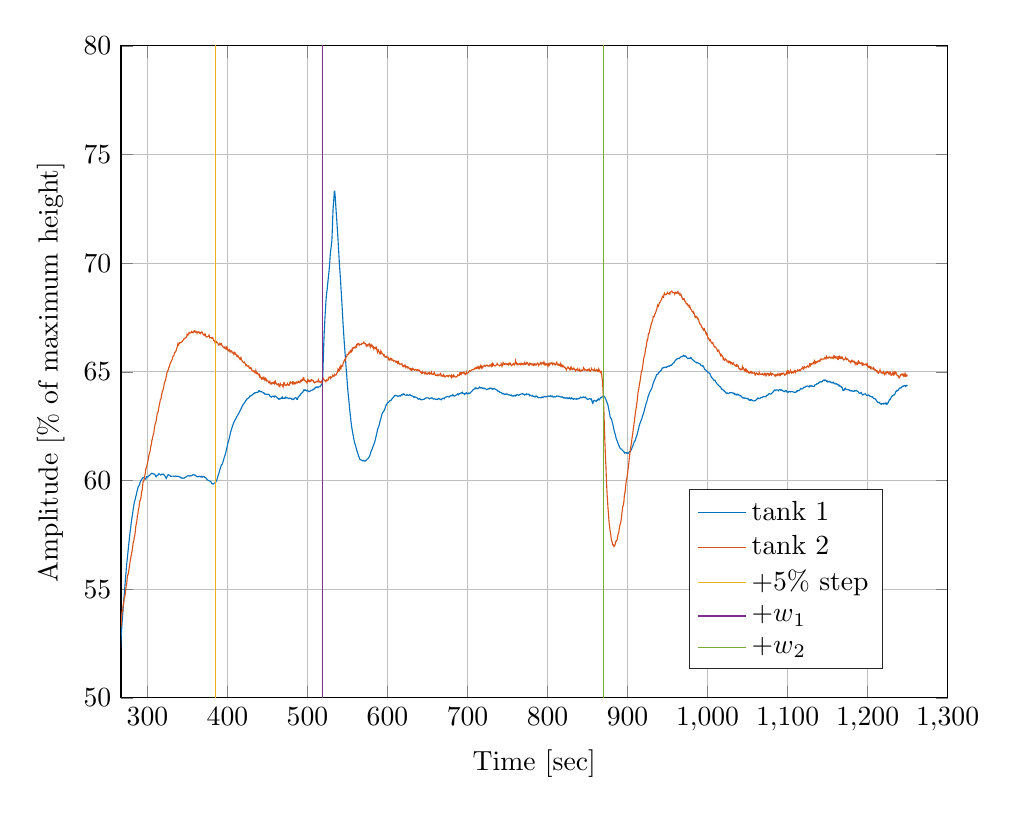
\begin{tikzpicture}

\begin{axis}[%
width=4.133in,
height=3.26in,
at={(0.693in,0.44in)},
scale only axis,
xmin=267,
xmax=1300,
xlabel={Time [sec]},
xmajorgrids,
ymin=50,
ymax=80,
ymajorgrids,
ylabel={Amplitude [$\%$ of maximum height]},
axis background/.style={fill=white},
legend style={at={(0.687,0.044)},anchor=south west,legend cell align=left,align=left,draw=white!15!black}
]
\addplot [color=mycolor1,solid]
  table[row sep=crcr]{%
0	0\\
0.5	5.99728834339049\\
1	8.20244057372836\\
1.5	9.04542956063184\\
2	9.43028711259504\\
2.5	9.64801141839532\\
3	10.1931326095926\\
3.5	10.9396410968746\\
4	11.7254522544269\\
4.5	12.4872166978117\\
5	13.5257410027077\\
5.5	14.940097623029\\
6	16.7896607236861\\
6.5	18.6166468346353\\
7	20.4980223778914\\
7.5	22.3911460645253\\
8	24.1717258724383\\
8.5	25.9645943310184\\
9	27.7429985376374\\
9.5	29.5487240256841\\
10	31.3083584779625\\
10.5	33.070163738985\\
11	34.8195819216052\\
11.5	36.6425489557396\\
12	38.4774452909203\\
12.5	40.3172122641799\\
13	42.0637488047735\\
13.5	43.7483789514017\\
14	45.4205867013254\\
14.5	47.0197929799166\\
15	48.6944672303606\\
15.5	50.3505721048977\\
16	51.9319386835954\\
16.5	53.5149302606766\\
17	54.8976332506875\\
17.5	56.2907778436965\\
18	57.5848477438255\\
18.5	58.7881377322902\\
19	59.9892001886055\\
19.5	61.2252663848498\\
20	62.4539412558704\\
20.5	63.5383283809723\\
21	64.5807050330422\\
21.5	65.6171968554835\\
22	66.6679417776706\\
22.5	67.5777272352485\\
23	68.3390128541229\\
23.5	69.1501543364742\\
24	69.8700438359407\\
24.5	70.7004057152576\\
25	71.5353338532298\\
25.5	72.5122274124557\\
26	74.0744131446682\\
26.5	76.2387529457812\\
27	77.7125548779117\\
27.5	78.507477441312\\
28	79.0092604903912\\
28.5	79.3691833488152\\
29	79.6749530787736\\
29.5	79.9322503466958\\
30	80.2108849277214\\
30.5	80.5120220631213\\
31	80.749002484929\\
31.5	80.9522775751445\\
32	81.1861414558718\\
32.5	81.4110416770638\\
33	81.6265319369429\\
33.5	81.8213655284211\\
34	82.055088596473\\
34.5	82.2759470165778\\
35	82.529174180109\\
35.5	82.7788910097535\\
36	83.0481060879444\\
36.5	83.3321668053474\\
37	83.6189571198236\\
37.5	83.9414875025995\\
38	84.2400502592107\\
38.5	84.5720057073569\\
39	84.8861092900365\\
39.5	85.2066672902073\\
40	85.5597156967826\\
40.5	85.9362145241177\\
41	86.3095198039134\\
41.5	86.6706924689449\\
42	87.0268345525262\\
42.5	87.4037088356362\\
43	87.7791866616954\\
43.5	88.1702979894256\\
44	88.5836850788725\\
44.5	88.9775486988621\\
45	89.371822781075\\
45.5	89.7750895443998\\
46	90.1601730818449\\
46.5	90.5318210647421\\
47	90.9312754629217\\
47.5	91.2983065913437\\
48	91.8735991035925\\
48.5	92.7705750932944\\
49	93.3901455041753\\
49.5	93.8147601250586\\
50	94.1580993285373\\
50.5	94.488151169922\\
51	94.8084457498295\\
51.5	95.2343416980723\\
52	95.6883326007736\\
52.5	96.44264766488\\
53	97.5259466659215\\
53.5	98.7032252742318\\
54	99.9480065600195\\
54.5	101.148346967214\\
55	102.200190637504\\
55.5	103.048870351825\\
56	103.741775027712\\
56.5	104.391367402338\\
57	104.974691392093\\
57.5	105.423361323371\\
58	105.750952348865\\
58.5	105.937949532478\\
59	106.033672577978\\
59.5	106.033009347679\\
60	106.045445255512\\
60.5	106.10777013987\\
61	106.229707708902\\
61.5	106.618160520881\\
62	107.970887021321\\
62.5	108.789976644362\\
63	108.767085005498\\
63.5	108.318678866233\\
64	107.688769198314\\
64.5	106.958364281488\\
65	106.207797217201\\
65.5	105.454799836692\\
66	104.688735033591\\
66.5	103.972648438337\\
67	103.264142788279\\
67.5	102.556917110054\\
68	101.935790656524\\
68.5	101.353628976977\\
69	100.794129690757\\
69.5	100.255747092753\\
70	99.7383942570708\\
70.5	99.2102968479322\\
71	98.7033194084597\\
71.5	98.2189405095819\\
72	97.7473199845062\\
72.5	97.3210412888212\\
73	96.900814190757\\
73.5	96.5222230636075\\
74	96.177697225832\\
74.5	95.7918148455678\\
75	95.437236359827\\
75.5	95.0952114382592\\
76	94.802705999744\\
76.5	94.5169028177369\\
77	94.2831345299476\\
77.5	94.0370942471842\\
78	93.8324133043504\\
78.5	93.6116834118079\\
79	93.4134570545197\\
79.5	93.2179811767758\\
80	93.0351861432229\\
80.5	92.8270270700735\\
81	92.7030387296304\\
81.5	92.5263841925488\\
82	92.3826779699485\\
82.5	92.2544070064134\\
83	92.1362878585869\\
83.5	92.0451257044659\\
84	91.9746703714415\\
84.5	91.8894733565475\\
85	91.8255811227307\\
85.5	91.756315294234\\
86	91.6665122168813\\
86.5	91.6127384160522\\
87	91.5517812271358\\
87.5	91.5127294803007\\
88	91.4801139014131\\
88.5	91.4534066970142\\
89	91.3976400501892\\
89.5	91.3620340340745\\
90	91.3459274743208\\
90.5	91.3469231214909\\
91	91.3428394618152\\
91.5	91.3280104089067\\
92	91.3713438738789\\
92.5	91.3942347046121\\
93	91.3893065634498\\
93.5	91.3887675914104\\
94	91.414316231559\\
94.5	91.4256707666587\\
95	91.4603924529041\\
95.5	91.4550175729725\\
96	91.4752222691732\\
96.5	91.5080722838206\\
97	91.5445268074783\\
97.5	91.6001843458439\\
98	91.6572522813167\\
98.5	91.6961618609187\\
99	91.7472664443683\\
99.5	91.7863624427046\\
100	91.8662990772523\\
100.5	91.9331243605823\\
101	92.0058311641535\\
101.5	92.08031445522\\
102	92.1429154528887\\
102.5	92.2260159864625\\
103	92.2953360703063\\
103.5	92.3347550432268\\
104	92.4070027518274\\
104.5	92.4829802086835\\
105	92.5416406462837\\
105.5	92.6196429381306\\
106	92.6870163641477\\
106.5	92.7703842280185\\
107	92.8045558530233\\
107.5	92.8589518361539\\
108	92.9528315036654\\
108.5	93.0546952829052\\
109	93.135059489218\\
109.5	93.1724263813674\\
110	93.2770782306417\\
110.5	93.3571150485926\\
111	93.4507313824255\\
111.5	93.5113937908432\\
112	93.5969705474433\\
112.5	93.6946258478018\\
113	93.7667007033724\\
113.5	93.8065916335011\\
114	93.9097001954593\\
114.5	94.0076004058845\\
115	94.1048309188276\\
115.5	94.1717544456879\\
116	94.2459706448987\\
116.5	94.2454778934655\\
117	94.2695844130658\\
117.5	94.2708407438047\\
118	94.2759397403221\\
118.5	94.2821030252518\\
119	94.2419859276864\\
119.5	94.2563268460648\\
120	94.2350101925021\\
120.5	94.1692560000931\\
121	94.1405586171432\\
121.5	94.0804708667503\\
122	93.9989677355968\\
122.5	93.9136529778723\\
123	93.8405516503839\\
123.5	93.774377751961\\
124	93.6854777556627\\
124.5	93.5809872477648\\
125	93.4734974343945\\
125.5	93.3382513385489\\
126	93.2163810306639\\
126.5	93.0730466990485\\
127	92.9524298476957\\
127.5	92.8300082506332\\
128	92.7075393429674\\
128.5	92.5575825335452\\
129	92.3903494128783\\
129.5	92.2476054701507\\
130	92.0708977199464\\
130.5	91.8971579800731\\
131	91.747823981873\\
131.5	91.5695465373663\\
132	91.4238930461566\\
132.5	91.2391668615946\\
133	91.0254084170235\\
133.5	90.8308399230072\\
134	90.6533861951273\\
134.5	90.465882692482\\
135	90.288984647614\\
135.5	90.1063696132246\\
136	89.915084592938\\
136.5	89.7055777889605\\
137	89.4955698513899\\
137.5	89.3089102885104\\
138	89.2667420895275\\
138.5	89.2236735574678\\
139	89.2766270266233\\
139.5	89.2575625353853\\
140	89.155230508869\\
140.5	89.0337504060955\\
141	88.8056419330839\\
141.5	88.5894433157303\\
142	88.397262147172\\
142.5	88.2016236504968\\
143	88.0336828133996\\
143.5	87.8612591162665\\
144	87.6913547270173\\
144.5	87.5079043770246\\
145	87.278479624256\\
145.5	87.0792427546778\\
146	86.8916131513759\\
146.5	86.6496002326823\\
147	86.4281758432042\\
147.5	86.2229510781914\\
148	86.0459577033028\\
148.5	85.8839516978372\\
149	85.6766423171439\\
149.5	85.4810766370009\\
150	85.3321248114112\\
150.5	85.2779672793287\\
151	85.2272959242331\\
151.5	85.1903544703669\\
152	85.1866462879609\\
152.5	85.1483614659004\\
153	85.1058960930966\\
153.5	85.0214021540894\\
154	84.9196849750933\\
154.5	84.950192900028\\
155	85.1730396376055\\
155.5	85.4586241082671\\
156	85.7593076902899\\
156.5	86.1247540908902\\
157	86.3766233799578\\
157.5	86.497871694671\\
158	86.5814257778466\\
158.5	86.6926912172806\\
159	86.8272726956087\\
159.5	86.971025026232\\
160	87.1559644667353\\
160.5	87.2866673451578\\
161	87.4036039540289\\
161.5	87.4887863911499\\
162	87.6126578294455\\
162.5	87.7445900825978\\
163	87.8631991462891\\
163.5	88.0145038424076\\
164	88.1595200946842\\
164.5	88.2986051584068\\
165	88.4118266454094\\
165.5	88.4993909459165\\
166	88.5743790680862\\
166.5	88.6127081686451\\
167	88.6834892185234\\
167.5	88.745637093061\\
168	88.8150028002808\\
168.5	88.8750233319398\\
169	88.9619272405305\\
169.5	88.9612328447873\\
170	88.9343582866778\\
170.5	88.9260355710514\\
171	88.9130477477853\\
171.5	88.9106388313148\\
172	88.9595876537604\\
172.5	89.0405801380029\\
173	89.1792907671786\\
173.5	89.2737742395686\\
174	89.4774818521666\\
174.5	89.697043943965\\
175	89.9127578629267\\
175.5	90.2589149994821\\
176	90.7213365691723\\
176.5	91.2380149871993\\
177	91.7691089081051\\
177.5	92.2738625053536\\
178	92.824537656841\\
178.5	93.2949184864241\\
179	93.6794258162962\\
179.5	93.9643662957218\\
180	94.2202229925131\\
180.5	94.4765437703278\\
181	94.800062383632\\
181.5	95.0831589317127\\
182	95.3245429362008\\
182.5	95.5725078578499\\
183	95.7955573955633\\
183.5	95.987494295018\\
184	96.1257955379499\\
184.5	96.2742004418077\\
185	96.4257570717201\\
185.5	96.5670555395529\\
186	96.6069281556973\\
186.5	96.5940774087893\\
187	96.6184635301383\\
187.5	96.5794664296558\\
188	96.5248157166009\\
188.5	96.4052944985309\\
189	96.3027171078487\\
189.5	96.2190797781419\\
190	96.1135278924041\\
190.5	95.9333682927979\\
191	95.7761343388353\\
191.5	95.5788012486749\\
192	95.3859786289559\\
192.5	95.1535080249209\\
193	94.9086102484673\\
193.5	94.63148070668\\
194	94.3545048547597\\
194.5	94.0252870286793\\
195	93.701331081662\\
195.5	93.2984827869937\\
196	92.8734907391684\\
196.5	92.4449935007029\\
197	91.9927869776827\\
197.5	91.4667905902893\\
198	90.9062099962285\\
198.5	90.1882288539357\\
199	89.2030617906808\\
199.5	88.0914405039386\\
200	86.8308006799962\\
200.5	85.5194912577265\\
201	84.1994191991058\\
201.5	82.8595493871144\\
202	81.4900035756187\\
202.5	80.1301623679484\\
203	78.7626205708424\\
203.5	77.3900917001165\\
204	76.0392290736828\\
204.5	74.7408106857507\\
205	73.4920647178867\\
205.5	72.2507635490149\\
206	71.0160123098606\\
206.5	69.8179271172316\\
207	68.6310230105527\\
207.5	67.4918643101245\\
208	66.3912805043086\\
208.5	65.2854587588321\\
209	64.2033944281715\\
209.5	63.1663723263106\\
210	62.1248938599283\\
210.5	61.1233406831015\\
211	60.1863637296537\\
211.5	59.2617045959775\\
212	58.3714540198726\\
212.5	57.4913348339731\\
213	56.6412292990197\\
213.5	55.8171801188958\\
214	54.9978551191662\\
214.5	54.2121606922607\\
215	53.4429344047566\\
215.5	52.6823370552741\\
216	51.9701585777267\\
216.5	51.2696281954373\\
217	50.617035035104\\
217.5	49.9434876748489\\
218	49.3015517198771\\
218.5	48.6903212151602\\
219	48.0985946089832\\
219.5	47.5208393390924\\
220	46.9359121080944\\
220.5	46.3699460556829\\
221	45.850894802144\\
221.5	45.3455192694324\\
222	44.8564344917745\\
222.5	44.3779270024804\\
223	43.9478178230179\\
223.5	43.4877127525479\\
224	43.0536273056432\\
224.5	42.6603665802988\\
225	42.2753896734291\\
225.5	41.8867188768129\\
226	41.5313629122272\\
226.5	41.1896988602911\\
227	40.8599463630943\\
227.5	40.5278910859253\\
228	40.2064724062795\\
228.5	39.9238279834399\\
229	39.625773148075\\
229.5	39.3429791749383\\
230	39.0841796464245\\
230.5	38.8441208345521\\
231	38.5988509119361\\
231.5	38.3879800034643\\
232	38.155065728079\\
232.5	37.9500186337736\\
233	37.7475460724488\\
233.5	37.5317279216232\\
234	37.3293147884659\\
234.5	37.1249594294023\\
235	36.9636680090055\\
235.5	36.7972276202\\
236	36.6485789457096\\
236.5	36.4990756550325\\
237	36.342088086653\\
237.5	36.1985611891913\\
238	36.0708404960976\\
238.5	35.9594853221693\\
239	35.8235590293503\\
239.5	35.6920756895614\\
240	35.5519798006729\\
240.5	35.4481879350773\\
241	35.3430526099531\\
241.5	35.2283439297133\\
242	35.118123284473\\
242.5	35.0461613248367\\
243	34.976508919696\\
243.5	34.9537539263445\\
244	34.9606139264806\\
244.5	35.0772381398218\\
245	35.2615757079777\\
245.5	35.535166806478\\
246	35.9010188884342\\
246.5	36.3050994414246\\
247	36.7422513405973\\
247.5	37.1711234045112\\
248	37.582256552465\\
248.5	37.9146997709442\\
249	38.2505103261541\\
249.5	38.6628366846302\\
250	39.1670539996538\\
250.5	39.6738482429787\\
251	40.1952261013084\\
251.5	40.8406238570637\\
252	41.4141628721987\\
252.5	41.9788236797613\\
253	42.4446587898004\\
253.5	42.9062692880153\\
254	43.3221882826319\\
254.5	43.7948610820198\\
255	44.1945104008623\\
255.5	44.606768957632\\
256	45.0334044206218\\
256.5	45.4208936169225\\
257	45.8230949705939\\
257.5	46.2482963766284\\
258	46.6495917521107\\
258.5	47.0212796803297\\
259	47.4564219097544\\
259.5	47.8019428549452\\
260	48.126793202915\\
260.5	48.4797551335222\\
261	48.8465533208442\\
261.5	49.2006044370851\\
262	49.5507022171667\\
262.5	49.8959710011532\\
263	50.207021155183\\
263.5	50.5844973567225\\
264	50.9210473618203\\
264.5	51.2164353174468\\
265	51.5200041943259\\
265.5	51.8010547072878\\
266	52.1193715518624\\
266.5	52.4086746906189\\
267	52.7045691115802\\
267.5	52.9776505644429\\
268	53.2650517653137\\
268.5	53.5344403658747\\
269	53.7859756739832\\
269.5	54.0115603353811\\
270	54.2686672490909\\
270.5	54.5296353455804\\
271	54.7461337565558\\
271.5	54.9455429775106\\
272	55.216555072345\\
272.5	55.4523283524668\\
273	55.6587884453649\\
273.5	55.8981136651851\\
274	56.1145405261651\\
274.5	56.2993859601809\\
275	56.4680871999276\\
275.5	56.6407568906051\\
276	56.8199218463901\\
276.5	57.0113099420196\\
277	57.1795708068872\\
277.5	57.3504893658208\\
278	57.5264347624116\\
278.5	57.6821126643886\\
279	57.8084253548889\\
279.5	57.9751929205193\\
280	58.1247556792543\\
280.5	58.2447692077125\\
281	58.3562541945304\\
281.5	58.4783704693445\\
282	58.6062066336727\\
282.5	58.7497529583437\\
283	58.8494240466096\\
283.5	58.9670426360791\\
284	59.0467416982892\\
284.5	59.1072770222262\\
285	59.1764006224753\\
285.5	59.2657821696588\\
286	59.3226217476316\\
286.5	59.410998690247\\
287	59.5010212003913\\
287.5	59.5544486362349\\
288	59.6385662186766\\
288.5	59.7018319333187\\
289	59.7393825554877\\
289.5	59.7629105012123\\
290	59.799805328324\\
290.5	59.8603391186218\\
291	59.9217371512216\\
291.5	59.9749183695353\\
292	59.9881038485337\\
292.5	60.0323773353982\\
293	60.0523441562003\\
293.5	60.0842719069396\\
294	60.1173134666717\\
294.5	60.1202939922543\\
295	60.1278742495995\\
295.5	60.1246751315054\\
296	60.1282178223954\\
296.5	60.0992866239077\\
297	60.0833314351851\\
297.5	60.0706270290728\\
298	60.0546620818163\\
298.5	60.1236331092686\\
299	60.1692324093883\\
299.5	60.1655796614981\\
300	60.1553171027925\\
300.5	60.1558284395736\\
301	60.1841112320635\\
301.5	60.202817998842\\
302	60.2233838101408\\
302.5	60.2231812659013\\
303	60.2482793736125\\
303.5	60.2642948310245\\
304	60.2811059583632\\
304.5	60.3050520700404\\
305	60.3189947934065\\
305.5	60.3336880304016\\
306	60.3199974994383\\
306.5	60.3173685029794\\
307	60.2992169032517\\
307.5	60.2951734425397\\
308	60.3043912340904\\
308.5	60.302116339488\\
309	60.2878328835969\\
309.5	60.2707880570994\\
310	60.2115519276698\\
310.5	60.1769975731109\\
311	60.1684898075535\\
311.5	60.201448310962\\
312	60.225329039626\\
312.5	60.2328555291327\\
313	60.2366252745423\\
313.5	60.2780604298536\\
314	60.3055466400487\\
314.5	60.2995296426883\\
315	60.2979964872917\\
315.5	60.2873450787303\\
316	60.2637444837635\\
316.5	60.252337415215\\
317	60.2557210108086\\
317.5	60.266705420071\\
318	60.2919417790171\\
318.5	60.2900823493235\\
319	60.2802288487589\\
319.5	60.2809140753636\\
320	60.29127666999\\
320.5	60.2712237386487\\
321	60.248511037153\\
321.5	60.2128920995407\\
322	60.1954542631642\\
322.5	60.1697012651046\\
323	60.1279097026034\\
323.5	60.0952235143785\\
324	60.1357213017629\\
324.5	60.171922244486\\
325	60.215461638832\\
325.5	60.2496358929966\\
326	60.2589127255028\\
326.5	60.2526460882726\\
327	60.2531869478951\\
327.5	60.2311748441699\\
328	60.2280052888861\\
328.5	60.2103010233249\\
329	60.1877568609805\\
329.5	60.1803894376241\\
330	60.1891920156751\\
330.5	60.1962109404202\\
331	60.198502873175\\
331.5	60.199967648193\\
332	60.1974091633778\\
332.5	60.2001516663085\\
333	60.1867910924558\\
333.5	60.1784973188433\\
334	60.1831408326743\\
334.5	60.2037194955439\\
335	60.2020084232771\\
335.5	60.1922164042086\\
336	60.1879934247778\\
336.5	60.1977794206301\\
337	60.1902591573953\\
337.5	60.1905335935771\\
338	60.1903153900005\\
338.5	60.1862701958296\\
339	60.1863390763086\\
339.5	60.1884652667661\\
340	60.1697826011102\\
340.5	60.1583633027902\\
341	60.1478399511782\\
341.5	60.1263787468396\\
342	60.1321177627292\\
342.5	60.1185676868483\\
343	60.1011217310118\\
343.5	60.1163758764105\\
344	60.1075946751464\\
344.5	60.1070497747048\\
345	60.1050081901712\\
345.5	60.1008961780787\\
346	60.1114142239751\\
346.5	60.126588002395\\
347	60.1425021929363\\
347.5	60.150767960587\\
348	60.1535205717085\\
348.5	60.1685463757423\\
349	60.1759726913771\\
349.5	60.2015726688117\\
350	60.2099772013264\\
350.5	60.2072015704943\\
351	60.2133552036227\\
351.5	60.216897078438\\
352	60.2063467140583\\
352.5	60.1976373578127\\
353	60.2055505656723\\
353.5	60.2102750881841\\
354	60.2203860709872\\
354.5	60.2131880077529\\
355	60.2157622877845\\
355.5	60.2278185914835\\
356	60.2357906029271\\
356.5	60.2527725539863\\
357	60.2566617381705\\
357.5	60.2690496870569\\
358	60.2575958754766\\
358.5	60.2515763545882\\
359	60.2542208555299\\
359.5	60.2482427979194\\
360	60.2288880431336\\
360.5	60.21519510419\\
361	60.1971823879544\\
361.5	60.18341272764\\
362	60.1718153082712\\
362.5	60.1695372252581\\
363	60.1828017501268\\
363.5	60.1698697163616\\
364	60.1816610931795\\
364.5	60.1888126815831\\
365	60.1911959585735\\
365.5	60.178968936359\\
366	60.179646787949\\
366.5	60.1745921604676\\
367	60.1524461437503\\
367.5	60.1825748543177\\
368	60.1912717595067\\
368.5	60.1741968675578\\
369	60.156679554502\\
369.5	60.1685432073894\\
370	60.1742136263231\\
370.5	60.1875740683045\\
371	60.1693175085471\\
371.5	60.1428509316125\\
372	60.1301320750751\\
372.5	60.1214929637642\\
373	60.1105444221725\\
373.5	60.1025141050822\\
374	60.0667062966433\\
374.5	60.0423196337846\\
375	60.0312273864991\\
375.5	60.0153567438269\\
376	60.0016354866998\\
376.5	59.99743884785\\
377	59.979133037043\\
377.5	59.9766971655611\\
378	59.9710645010246\\
378.5	59.9577173173902\\
379	59.9520925141307\\
379.5	59.9333638983134\\
380	59.8762184547345\\
380.5	59.8577903953726\\
381	59.8558496363058\\
381.5	59.8341051708027\\
382	59.8315206304411\\
382.5	59.8397118895702\\
383	59.8634677091061\\
383.5	59.877730829811\\
384	59.8764867532079\\
384.5	59.8945511990046\\
385	59.9069392026462\\
385.5	59.9421632764497\\
386	59.9670192900646\\
386.5	60.0078041689634\\
387	60.0487467272476\\
387.5	60.1147886926106\\
388	60.1927752770239\\
388.5	60.2435156660425\\
389	60.2900728855097\\
389.5	60.3556082738628\\
390	60.4209546771859\\
390.5	60.5021224609585\\
391	60.5406127773325\\
391.5	60.6113581232305\\
392	60.6626425081051\\
392.5	60.6935215020041\\
393	60.734619488485\\
393.5	60.7562933957313\\
394	60.8077565510004\\
394.5	60.8675073244205\\
395	60.9265944680735\\
395.5	60.9900564499253\\
396	61.0585278125557\\
396.5	61.1252992466859\\
397	61.1557556088736\\
397.5	61.2268846412409\\
398	61.2936371916428\\
398.5	61.3719003641023\\
399	61.4656263775923\\
399.5	61.5420349637716\\
400	61.6228328032273\\
400.5	61.7109719528465\\
401	61.7770308413006\\
401.5	61.8313807248195\\
402	61.9013931185409\\
402.5	61.9689759826759\\
403	62.0498571820383\\
403.5	62.1516120681438\\
404	62.2335034739809\\
404.5	62.2829343305577\\
405	62.3418559414803\\
405.5	62.401543585185\\
406	62.471874183697\\
406.5	62.5228778049525\\
407	62.5773991079078\\
407.5	62.62360607578\\
408	62.6696509872446\\
408.5	62.7038642545596\\
409	62.7450638827797\\
409.5	62.7894278753473\\
410	62.8077097948633\\
410.5	62.8387092146573\\
411	62.8941900007073\\
411.5	62.9217060511102\\
412	62.9668131464829\\
412.5	62.9836774364854\\
413	63.0121845289329\\
413.5	63.0504812751925\\
414	63.0853050761027\\
414.5	63.1059899927754\\
415	63.148793641433\\
415.5	63.1862267655764\\
416	63.2280634811586\\
416.5	63.2500959906097\\
417	63.2950820098142\\
417.5	63.3491056225305\\
418	63.3836935516784\\
418.5	63.4169993042588\\
419	63.4429248734735\\
419.5	63.4926440058222\\
420	63.5149407817965\\
420.5	63.5314725406752\\
421	63.5556142411165\\
421.5	63.5895032301907\\
422	63.6212110233724\\
422.5	63.6322415542561\\
423	63.6871791871479\\
423.5	63.6982984667526\\
424	63.7091097643766\\
424.5	63.7554045023766\\
425	63.7619627364743\\
425.5	63.7688809018474\\
426	63.7882254278951\\
426.5	63.8035653519156\\
427	63.8176586617409\\
427.5	63.8449821767477\\
428	63.8871786524044\\
428.5	63.8831166848926\\
429	63.8825925090663\\
429.5	63.9057542439248\\
430	63.9027778264747\\
430.5	63.9250825056942\\
431	63.9373821933083\\
431.5	63.9522951386742\\
432	63.9702952221067\\
432.5	63.9819336164697\\
433	64.0081233041374\\
433.5	64.0138553414352\\
434	64.0331302496808\\
434.5	64.0234785965285\\
435	64.0276604675511\\
435.5	64.0482890648\\
436	64.0471796015329\\
436.5	64.0459821163983\\
437	64.0552604213015\\
437.5	64.0492711305273\\
438	64.0602788568963\\
438.5	64.0765530722314\\
439	64.1196387535299\\
439.5	64.1375063487965\\
440	64.1227389061659\\
440.5	64.0966263974159\\
441	64.0795410254556\\
441.5	64.0868042504435\\
442	64.0990611932485\\
442.5	64.0838193052282\\
443	64.0691889764473\\
443.5	64.0665908517385\\
444	64.066688288814\\
444.5	64.0501795181942\\
445	64.0273652065457\\
445.5	64.0344520946929\\
446	64.0084197092548\\
446.5	63.9779986675691\\
447	63.968411338489\\
447.5	63.9788505747046\\
448	63.9691408549557\\
448.5	63.9634381556077\\
449	63.9599485068138\\
449.5	63.9623008226261\\
450	63.9735176526641\\
450.5	63.9709267958104\\
451	63.964595592791\\
451.5	63.9569998236482\\
452	63.9471272999643\\
452.5	63.9192504799109\\
453	63.8916241687697\\
453.5	63.8601755660663\\
454	63.8568452973571\\
454.5	63.8433838017113\\
455	63.8311900335999\\
455.5	63.852945272844\\
456	63.870847981759\\
456.5	63.8687789213196\\
457	63.8819879955561\\
457.5	63.8716142238097\\
458	63.8595149064196\\
458.5	63.8387570971674\\
459	63.8663909457399\\
459.5	63.8901608680941\\
460	63.8734169444559\\
460.5	63.8714229045487\\
461	63.8459665523053\\
461.5	63.8268637735706\\
462	63.8184492581902\\
462.5	63.7886335885771\\
463	63.7848559703921\\
463.5	63.764982620957\\
464	63.7413900346963\\
464.5	63.731805699327\\
465	63.77334297072\\
465.5	63.7756038422418\\
466	63.755977934729\\
466.5	63.7650410076434\\
467	63.787447749405\\
467.5	63.7765786117236\\
468	63.7809046853104\\
468.5	63.8416783951593\\
469	63.8111069876828\\
469.5	63.7796153355927\\
470	63.7782899193772\\
470.5	63.7806133009332\\
471	63.7908467341074\\
471.5	63.7737745163311\\
472	63.7713097549813\\
472.5	63.8219511288449\\
473	63.8379343074583\\
473.5	63.8129467917492\\
474	63.7943829407765\\
474.5	63.7991956609911\\
475	63.8038025420459\\
475.5	63.7894516935819\\
476	63.7805337971893\\
476.5	63.7639648428567\\
477	63.7628999865929\\
477.5	63.7827877497356\\
478	63.7908567030598\\
478.5	63.7774558480701\\
479	63.778338288784\\
479.5	63.774108577428\\
480	63.7583088008611\\
480.5	63.7408141375328\\
481	63.7518851529975\\
481.5	63.746420105423\\
482	63.7205150186247\\
482.5	63.7181810678995\\
483	63.7435565091891\\
483.5	63.7711328977605\\
484	63.7866457262659\\
484.5	63.7970637871802\\
485	63.809107980611\\
485.5	63.8063260863097\\
486	63.7897054567414\\
486.5	63.7419123381415\\
487	63.7274406332783\\
487.5	63.7347475366272\\
488	63.8002758571911\\
488.5	63.841087076343\\
489	63.8441928878238\\
489.5	63.8778828503119\\
490	63.9125040264411\\
490.5	63.9193937021333\\
491	63.9321385109689\\
491.5	63.980889183902\\
492	63.9865102427028\\
492.5	64.017604710491\\
493	64.0224420000472\\
493.5	64.0389590847046\\
494	64.0556277156138\\
494.5	64.0943437967298\\
495	64.1246609590801\\
495.5	64.160095630325\\
496	64.1443114794985\\
496.5	64.140140076295\\
497	64.1695624028224\\
497.5	64.1523415530644\\
498	64.1434882433773\\
498.5	64.1343787639664\\
499	64.1216501747992\\
499.5	64.1351470083181\\
500	64.1498947236255\\
500.5	64.1237086034847\\
501	64.1065830111129\\
501.5	64.0860317211483\\
502	64.0917936169943\\
502.5	64.1071495673024\\
503	64.104421931248\\
503.5	64.1200867634829\\
504	64.1235076879031\\
504.5	64.1483588746348\\
505	64.1444758950176\\
505.5	64.1502242844688\\
506	64.1589764112398\\
506.5	64.176277080946\\
507	64.192101866309\\
507.5	64.1753757773516\\
508	64.1835575517462\\
508.5	64.2289574891055\\
509	64.2480793727246\\
509.5	64.2456493008448\\
510	64.2792489653634\\
510.5	64.2822928934823\\
511	64.3016944936041\\
511.5	64.3009266075655\\
512	64.2887008656919\\
512.5	64.2981006967811\\
513	64.2742660776844\\
513.5	64.2848062481469\\
514	64.3041129418323\\
514.5	64.306383533635\\
515	64.3238468012357\\
515.5	64.3243902247347\\
516	64.3252240750904\\
516.5	64.349962340406\\
517	64.3760218901028\\
517.5	64.4149296026929\\
518	64.4280435012653\\
518.5	64.4293241429895\\
519	64.6413016668525\\
519.5	65.2510650091426\\
520	65.8521875944499\\
520.5	66.4166455060343\\
521	66.8589063643645\\
521.5	67.2219355677772\\
522	67.5671686666653\\
522.5	67.8901998104233\\
523	68.1942876491765\\
523.5	68.4583842745154\\
524	68.6244398243744\\
524.5	68.7536844762621\\
525	68.9342846165602\\
525.5	69.1378543331196\\
526	69.3014691799197\\
526.5	69.4783496106847\\
527	69.6539535671909\\
527.5	69.8686366449839\\
528	70.1087269030874\\
528.5	70.3948678777349\\
529	70.5761740468305\\
529.5	70.7109865019324\\
530	70.8772029444345\\
530.5	71.0476699406742\\
531	71.4741034938521\\
531.5	72.0475429863346\\
532	72.4821816785773\\
532.5	72.739960314778\\
533	72.9775966364795\\
533.5	73.2860837444645\\
534	73.3027741477255\\
534.5	73.1281917678546\\
535	72.8766955040155\\
535.5	72.5769639561234\\
536	72.2892130276596\\
536.5	72.0412696461168\\
537	71.7637335744312\\
537.5	71.4792213591062\\
538	71.1799626980916\\
538.5	70.8583848208712\\
539	70.5591518588606\\
539.5	70.2265835762475\\
540	69.9136682979298\\
540.5	69.6575699989335\\
541	69.3982680562054\\
541.5	69.1155207317603\\
542	68.7916818700796\\
542.5	68.4929954356421\\
543	68.1799644960691\\
543.5	67.8612726304885\\
544	67.5217332041399\\
544.5	67.2031579714939\\
545	66.9133130341155\\
545.5	66.6211981867298\\
546	66.3450407142238\\
546.5	66.0946228870699\\
547	65.8467322298989\\
547.5	65.6115207501683\\
548	65.3364086793621\\
548.5	65.0939348452926\\
549	64.8641154322132\\
549.5	64.6115305557521\\
550	64.3689915409876\\
550.5	64.1353265310256\\
551	63.9325006528326\\
551.5	63.7551434974777\\
552	63.5693899340889\\
552.5	63.3801584925365\\
553	63.1878903836533\\
553.5	63.0185500207013\\
554	62.8592658706525\\
554.5	62.6840385048755\\
555	62.5367846629487\\
555.5	62.4100284347643\\
556	62.3037092623517\\
556.5	62.185681168392\\
557	62.0953098933774\\
557.5	61.9943572384917\\
558	61.8980289088665\\
558.5	61.7967357789089\\
559	61.7234373389565\\
559.5	61.6725600817542\\
560	61.6203906456767\\
560.5	61.5383618226323\\
561	61.4758597350509\\
561.5	61.3972614914504\\
562	61.3457870971954\\
562.5	61.2922525860074\\
563	61.2413803669818\\
563.5	61.1685388373687\\
564	61.1064759845203\\
564.5	61.077474285966\\
565	61.0095332909235\\
565.5	60.9640013590899\\
566	60.9522967259582\\
566.5	60.947913030244\\
567	60.9461135516776\\
567.5	60.9377202278098\\
568	60.9243384661878\\
568.5	60.9094498354457\\
569	60.9028038507867\\
569.5	60.9101764390211\\
570	60.9096968698292\\
570.5	60.9260746137636\\
571	60.9034190888185\\
571.5	60.8926184110743\\
572	60.8925530716746\\
572.5	60.8973249549561\\
573	60.9178488216277\\
573.5	60.9329130010633\\
574	60.9595041290883\\
574.5	60.9718161986212\\
575	60.9908370106757\\
575.5	60.9986146075901\\
576	61.0307489039115\\
576.5	61.0395160143305\\
577	61.0734703835693\\
577.5	61.1197596657955\\
578	61.1605311724405\\
578.5	61.2228622431275\\
579	61.2752046245918\\
579.5	61.3464971365214\\
580	61.3833211908178\\
580.5	61.4192224880593\\
581	61.4497011088514\\
581.5	61.5198420649372\\
582	61.560821221619\\
582.5	61.6127688842622\\
583	61.6712198092876\\
583.5	61.7106009274049\\
584	61.7686520946349\\
584.5	61.8416014611924\\
585	61.9093647762391\\
585.5	61.995261502576\\
586	62.064573504679\\
586.5	62.157126280859\\
587	62.2387968480935\\
587.5	62.3240554824595\\
588	62.3882408657677\\
588.5	62.4395994394132\\
589	62.4721431611276\\
589.5	62.532928309582\\
590	62.6137535058881\\
590.5	62.6889014913693\\
591	62.7736654627749\\
591.5	62.8217690903407\\
592	62.882328804145\\
592.5	62.959521052208\\
593	63.0426391518912\\
593.5	63.0944593314566\\
594	63.1216541392659\\
594.5	63.1393422321201\\
595	63.174611382418\\
595.5	63.1989477484516\\
596	63.232875089041\\
596.5	63.2747635886756\\
597	63.3220096283199\\
597.5	63.3853682800437\\
598	63.431245546629\\
598.5	63.4892592670383\\
599	63.4980953219003\\
599.5	63.5380847152443\\
600	63.5593456906856\\
600.5	63.5739921938086\\
601	63.5892848316146\\
601.5	63.6093545469064\\
602	63.6341744241451\\
602.5	63.6524707147351\\
603	63.6731650286313\\
603.5	63.6823203148408\\
604	63.6814212320792\\
604.5	63.6945183171357\\
605	63.7123824642156\\
605.5	63.7457856014556\\
606	63.7816759903989\\
606.5	63.7968476830673\\
607	63.8182332391826\\
607.5	63.8331131175702\\
608	63.8530750898492\\
608.5	63.8803047151823\\
609	63.9141192230237\\
609.5	63.9194821253202\\
610	63.9057131267462\\
610.5	63.8977249388828\\
611	63.8914660747515\\
611.5	63.9025284876777\\
612	63.895546150677\\
612.5	63.885122681827\\
613	63.8676201105578\\
613.5	63.8739583117604\\
614	63.8862243244694\\
614.5	63.8850807056998\\
615	63.8951429921871\\
615.5	63.9019731144455\\
616	63.9003643197287\\
616.5	63.8874334683369\\
617	63.9221658900279\\
617.5	63.9440496690167\\
618	63.9513061638962\\
618.5	63.9647404342761\\
619	63.936425539614\\
619.5	63.9530669544645\\
620	63.9653259902676\\
620.5	63.9847860836591\\
621	63.9613030745805\\
621.5	63.9375555836446\\
622	63.9302369682498\\
622.5	63.9232819386904\\
623	63.9247806848952\\
623.5	63.921179675634\\
624	63.9362159407342\\
624.5	63.9522022195962\\
625	63.9329243863167\\
625.5	63.9190863459663\\
626	63.9231740574814\\
626.5	63.9248905188229\\
627	63.9212722677701\\
627.5	63.9261052474955\\
628	63.9497559513057\\
628.5	63.9255826862261\\
629	63.9136250532063\\
629.5	63.9133375666184\\
630	63.9039934972728\\
630.5	63.8870037455318\\
631	63.8904227203383\\
631.5	63.8770563962568\\
632	63.8660906080192\\
632.5	63.8435959639069\\
633	63.8222139298794\\
633.5	63.8346832922908\\
634	63.8530318742944\\
634.5	63.8411784517791\\
635	63.8385803024678\\
635.5	63.8271186853866\\
636	63.8145897023969\\
636.5	63.8069263267446\\
637	63.7991296543065\\
637.5	63.7803320773061\\
638	63.7513696311382\\
638.5	63.7483111062201\\
639	63.7381549269121\\
639.5	63.7403332771791\\
640	63.7621982087969\\
640.5	63.7611411770279\\
641	63.7410140509081\\
641.5	63.7170457228393\\
642	63.7099895483405\\
642.5	63.7114716350199\\
643	63.7089509427434\\
643.5	63.7305166842608\\
644	63.7310280277093\\
644.5	63.7306369678246\\
645	63.7300943014128\\
645.5	63.7330914951988\\
646	63.7480786322189\\
646.5	63.7670384677173\\
647	63.7706811353861\\
647.5	63.787013695938\\
648	63.7924020625486\\
648.5	63.7958441349081\\
649	63.8113971554176\\
649.5	63.8031217593192\\
650	63.7981664254254\\
650.5	63.7993243008954\\
651	63.7963598677901\\
651.5	63.7956656510025\\
652	63.7665039618591\\
652.5	63.7530492164943\\
653	63.7766888552448\\
653.5	63.778145670821\\
654	63.78772977155\\
654.5	63.7919425125176\\
655	63.7861454273839\\
655.5	63.8003659537249\\
656	63.7746973308927\\
656.5	63.77116463647\\
657	63.7539094626888\\
657.5	63.7473547579586\\
658	63.748466012624\\
658.5	63.7565612189114\\
659	63.7527257705378\\
659.5	63.7469098558682\\
660	63.7301677544951\\
660.5	63.7280305146573\\
661	63.7278684650026\\
661.5	63.738860397568\\
662	63.7285340180623\\
662.5	63.7224939194297\\
663	63.7449294472229\\
663.5	63.7597829884501\\
664	63.7778604530563\\
664.5	63.7672095472213\\
665	63.7474764115552\\
665.5	63.7481139814617\\
666	63.7431867670749\\
666.5	63.7162482633207\\
667	63.7146443783439\\
667.5	63.7114805254385\\
668	63.7609821517119\\
668.5	63.7702723602753\\
669	63.7791867222514\\
669.5	63.7778813233129\\
670	63.7816616586937\\
670.5	63.7591858787936\\
671	63.7604982233017\\
671.5	63.794650425302\\
672	63.8180383639985\\
672.5	63.8325813751962\\
673	63.8432294527898\\
673.5	63.8361252476002\\
674	63.8480982034397\\
674.5	63.8554114872664\\
675	63.8693474242001\\
675.5	63.8615348065811\\
676	63.8541566858634\\
676.5	63.8434503223875\\
677	63.8411401194793\\
677.5	63.8515646563789\\
678	63.8809580371961\\
678.5	63.8837779827747\\
679	63.897134440917\\
679.5	63.9090401055156\\
680	63.9028641256316\\
680.5	63.8911106092497\\
681	63.9168525805638\\
681.5	63.9427226628539\\
682	63.9380402329345\\
682.5	63.9013516430946\\
683	63.8903480783378\\
683.5	63.8811022488709\\
684	63.8854844501864\\
684.5	63.8936835835898\\
685	63.9051804316537\\
685.5	63.925268977698\\
686	63.9347332174703\\
686.5	63.9438462725065\\
687	63.9495324218235\\
687.5	63.9671873741039\\
688	63.986613373361\\
688.5	63.9398502373278\\
689	63.9470818030515\\
689.5	63.9807976287988\\
690	64.0000113206786\\
690.5	64.0091034882495\\
691	64.0084901097285\\
691.5	64.0223200783982\\
692	64.0225083446801\\
692.5	64.022673922719\\
693	64.0434009705223\\
693.5	64.0561726354921\\
694	64.0100956237994\\
694.5	64.0141160556522\\
695	64.00335821848\\
695.5	63.9999628860508\\
696	63.9751140582023\\
696.5	63.9574613816911\\
697	63.9801913843692\\
697.5	64.0052117519235\\
698	64.0285650492681\\
698.5	64.0370470575979\\
699	64.0090956618288\\
699.5	63.994389702704\\
700	63.9825016228959\\
700.5	63.9816619070476\\
701	63.993688159355\\
701.5	64.0203295165177\\
702	64.0013726837107\\
702.5	63.9969135077208\\
703	64.0216722548905\\
703.5	64.0339248883206\\
704	64.0456737213167\\
704.5	64.0714123166992\\
705	64.092218758821\\
705.5	64.1035430930837\\
706	64.1223187794417\\
706.5	64.1539733188125\\
707	64.1779294777751\\
707.5	64.1786644469838\\
708	64.2015628792264\\
708.5	64.2089455578567\\
709	64.2242255585248\\
709.5	64.2521608523538\\
710	64.2316571737477\\
710.5	64.2562386906312\\
711	64.252193021436\\
711.5	64.2378033863919\\
712	64.2205946414283\\
712.5	64.2258262273347\\
713	64.239334248879\\
713.5	64.2400724521893\\
714	64.2618541634264\\
714.5	64.2609320332684\\
715	64.2930982103186\\
715.5	64.2734810342804\\
716	64.2565439656468\\
716.5	64.2665024083471\\
717	64.2800365836192\\
717.5	64.2671574753696\\
718	64.2678831437226\\
718.5	64.2375443162539\\
719	64.2413851019058\\
719.5	64.2451742800912\\
720	64.2495375456865\\
720.5	64.227186782333\\
721	64.2462848003175\\
721.5	64.236877657358\\
722	64.2222084433274\\
722.5	64.2123658074561\\
723	64.2051381207871\\
723.5	64.1972507559787\\
724	64.1788120405631\\
724.5	64.1840228689315\\
725	64.2020370623134\\
725.5	64.1960971276465\\
726	64.2190198566297\\
726.5	64.2188159566144\\
727	64.2165747447518\\
727.5	64.2151919144341\\
728	64.2513649829623\\
728.5	64.2441795175465\\
729	64.2403407439636\\
729.5	64.2478754053567\\
730	64.2342545435024\\
730.5	64.2193392461188\\
731	64.1942531355771\\
731.5	64.2157851385501\\
732	64.2093598675927\\
732.5	64.2170486888734\\
733	64.2215643889399\\
733.5	64.2284066067958\\
734	64.2091943347321\\
734.5	64.2013324457464\\
735	64.1933926562955\\
735.5	64.1905986382551\\
736	64.1751424244542\\
736.5	64.170514449405\\
737	64.1518383024757\\
737.5	64.134247603364\\
738	64.1096411656672\\
738.5	64.0925134868149\\
739	64.1058726412058\\
739.5	64.1000147871045\\
740	64.0832715740287\\
740.5	64.0524453568126\\
741	64.0540171855418\\
741.5	64.0497849095104\\
742	64.0445179463774\\
742.5	64.024765000584\\
743	64.0076107494657\\
743.5	63.9878767658117\\
744	64.0008816580942\\
744.5	63.9843197534255\\
745	63.989413908799\\
745.5	63.9923521346731\\
746	63.9649902973016\\
746.5	63.9573011771848\\
747	63.9611582961517\\
747.5	63.9623125358795\\
748	63.9814624529846\\
748.5	63.968251975561\\
749	63.9806609793426\\
749.5	63.9719956518902\\
750	63.9734938088396\\
750.5	63.9544075724367\\
751	63.9391767547618\\
751.5	63.9339475056314\\
752	63.9434781294215\\
752.5	63.9402511614712\\
753	63.9242013354573\\
753.5	63.9242903216444\\
754	63.9168291143866\\
754.5	63.928566227396\\
755	63.9340565426216\\
755.5	63.8895167609655\\
756	63.8960682506745\\
756.5	63.8860769670408\\
757	63.8881050593147\\
757.5	63.8840239828034\\
758	63.8974372263654\\
758.5	63.9144714533774\\
759	63.91305858064\\
759.5	63.8835876462867\\
760	63.9051850569317\\
760.5	63.9210676819276\\
761	63.9118950161483\\
761.5	63.9323240852577\\
762	63.9493400957049\\
762.5	63.9367264080205\\
763	63.935675007024\\
763.5	63.9325165884448\\
764	63.9198199888566\\
764.5	63.924303783002\\
765	63.9515080864448\\
765.5	63.9542080721549\\
766	63.9630318139796\\
766.5	63.9666189005801\\
767	63.9753596326027\\
767.5	63.9831638114197\\
768	63.9921859526625\\
768.5	64.0029493395907\\
769	63.9904697752346\\
769.5	63.9682804087611\\
770	63.9721073098968\\
770.5	63.9627068060721\\
771	63.9439891633035\\
771.5	63.9317002809982\\
772	63.9618679148866\\
772.5	63.9550443226016\\
773	63.9645683059407\\
773.5	63.9537065934447\\
774	63.9824238290037\\
774.5	63.9759019231095\\
775	63.9725799911159\\
775.5	63.9649934412667\\
776	63.9673936023853\\
776.5	63.9768333115141\\
777	63.9537809700637\\
777.5	63.9075454606193\\
778	63.9290165848023\\
778.5	63.9134892574496\\
779	63.9145603037397\\
779.5	63.8922733647941\\
780	63.8874790467841\\
780.5	63.885882524837\\
781	63.8909405926988\\
781.5	63.9111845619577\\
782	63.8673084319816\\
782.5	63.8614047596368\\
783	63.8683245462001\\
783.5	63.8650576610215\\
784	63.8496622963832\\
784.5	63.8417826111628\\
785	63.8598080227287\\
785.5	63.8905484186413\\
786	63.8887862621765\\
786.5	63.8707100133606\\
787	63.8657901674846\\
787.5	63.833646731007\\
788	63.8144757809562\\
788.5	63.8002989081783\\
789	63.8158394958603\\
789.5	63.8142752269955\\
790	63.8095761326237\\
790.5	63.8155915890702\\
791	63.8152281064795\\
791.5	63.8029165590829\\
792	63.8047132123775\\
792.5	63.817984899483\\
793	63.840653524553\\
793.5	63.8423964536355\\
794	63.8145719239791\\
794.5	63.8161324790009\\
795	63.8344023493737\\
795.5	63.8554089388294\\
796	63.8650076558509\\
796.5	63.8522292559021\\
797	63.856047896301\\
797.5	63.8619669119393\\
798	63.8474403234267\\
798.5	63.8591092537894\\
799	63.8515354669743\\
799.5	63.8623747631214\\
800	63.8704510153758\\
800.5	63.8788192924655\\
801	63.8766414054494\\
801.5	63.8838294602976\\
802	63.8806542549651\\
802.5	63.8804199286455\\
803	63.8629334742241\\
803.5	63.8687672291674\\
804	63.897065725679\\
804.5	63.8812342183833\\
805	63.880854061566\\
805.5	63.8555504251833\\
806	63.8760031637566\\
806.5	63.8437697702326\\
807	63.8449347072048\\
807.5	63.8395923558747\\
808	63.8559955057456\\
808.5	63.8596583419656\\
809	63.8565876459753\\
809.5	63.839214801334\\
810	63.8417884121913\\
810.5	63.8484425604957\\
811	63.8844021522306\\
811.5	63.8893830251333\\
812	63.881632938888\\
812.5	63.8826457034365\\
813	63.8758742696769\\
813.5	63.8809842018677\\
814	63.8654850000703\\
814.5	63.8781190272006\\
815	63.8595855793795\\
815.5	63.8575456212108\\
816	63.8489699713186\\
816.5	63.8352164819415\\
817	63.8343987736729\\
817.5	63.8365203833937\\
818	63.8551395575705\\
818.5	63.8485632560849\\
819	63.8291746793643\\
819.5	63.8290180512747\\
820	63.8084683995945\\
820.5	63.789612785547\\
821	63.8040795211552\\
821.5	63.7901203791648\\
822	63.7845519752013\\
822.5	63.79180970725\\
823	63.8095505472257\\
823.5	63.7996925136095\\
824	63.7987731472714\\
824.5	63.7746469651903\\
825	63.7931441502382\\
825.5	63.7817684161869\\
826	63.7674686360611\\
826.5	63.7814019088493\\
827	63.8048504116237\\
827.5	63.8108948772436\\
828	63.7878607226265\\
828.5	63.7554757635054\\
829	63.7490000694489\\
829.5	63.7798909006541\\
830	63.7971008473392\\
830.5	63.7849821047213\\
831	63.7638193765501\\
831.5	63.7617779925143\\
832	63.7408820604043\\
832.5	63.7336018030845\\
833	63.7482477549649\\
833.5	63.7736368040127\\
834	63.7670544099994\\
834.5	63.7500159189367\\
835	63.7439330281185\\
835.5	63.7436903771205\\
836	63.7384295977537\\
836.5	63.7624165177218\\
837	63.7475678378985\\
837.5	63.7464183836048\\
838	63.752864621383\\
838.5	63.7652684705881\\
839	63.7797935052634\\
839.5	63.7631981902915\\
840	63.774422867239\\
840.5	63.7926358140865\\
841	63.80944631732\\
841.5	63.8276842862668\\
842	63.8083053212361\\
842.5	63.8065281050098\\
843	63.8149931570148\\
843.5	63.8273090053596\\
844	63.8249694339754\\
844.5	63.8435865614952\\
845	63.8453382702711\\
845.5	63.8231000076719\\
846	63.8151948778925\\
846.5	63.8182324299255\\
847	63.8369743330384\\
847.5	63.8086238017284\\
848	63.8014136163099\\
848.5	63.7781359303167\\
849	63.7572935998114\\
849.5	63.753960682843\\
850	63.7284843119938\\
850.5	63.7246965561147\\
851	63.743494568303\\
851.5	63.7501566509587\\
852	63.75059218583\\
852.5	63.7615208512668\\
853	63.7514092664018\\
853.5	63.7529001550505\\
854	63.7331107739577\\
854.5	63.7536208663943\\
855	63.7356694439766\\
855.5	63.6468393556054\\
856	63.5872596749605\\
856.5	63.5489285163066\\
857	63.580907337538\\
857.5	63.6634528949588\\
858	63.6755694845517\\
858.5	63.6843740633696\\
859	63.6743610287453\\
859.5	63.6516657361727\\
860	63.6553010901179\\
860.5	63.6555209631744\\
861	63.6445482303362\\
861.5	63.6576518373033\\
862	63.6997090146746\\
862.5	63.6937642783407\\
863	63.7355077593346\\
863.5	63.7492819966661\\
864	63.7188846472799\\
864.5	63.7057175792691\\
865	63.7252136485874\\
865.5	63.7651489152139\\
866	63.7937439747608\\
866.5	63.8092471549851\\
867	63.8108746605778\\
867.5	63.8140201719219\\
868	63.8389388651859\\
868.5	63.864466654222\\
869	63.8695782000865\\
869.5	63.8608390207882\\
870	63.8591285713636\\
870.5	63.8770513297814\\
871	63.8457914982672\\
871.5	63.8354000917686\\
872	63.8110874922351\\
872.5	63.7648970814903\\
873	63.7111886040111\\
873.5	63.6626418471014\\
874	63.6306922725042\\
874.5	63.5674213991026\\
875	63.5176824456524\\
875.5	63.4713288590674\\
876	63.366493293172\\
876.5	63.2861562169272\\
877	63.1858981270296\\
877.5	63.0779471080359\\
878	62.9788545653582\\
878.5	62.8908389486971\\
879	62.8654440827346\\
879.5	62.855793532822\\
880	62.8038551381911\\
880.5	62.7399755904071\\
881	62.6686076577479\\
881.5	62.5904622492518\\
882	62.5225581548052\\
882.5	62.4213777511241\\
883	62.3324247434687\\
883.5	62.2631670600355\\
884	62.1909173438565\\
884.5	62.1318788391058\\
885	62.0602977208652\\
885.5	61.978170968688\\
886	61.9131767229037\\
886.5	61.8645477613794\\
887	61.8197263301973\\
887.5	61.7723744883171\\
888	61.7071379272265\\
888.5	61.6750096440749\\
889	61.6179213409397\\
889.5	61.5900059550239\\
890	61.5410153250826\\
890.5	61.4967732245365\\
891	61.4713286191164\\
891.5	61.4552002206559\\
892	61.4442637157754\\
892.5	61.4389335286551\\
893	61.4102772465632\\
893.5	61.391507892599\\
894	61.3743418174155\\
894.5	61.3508854287587\\
895	61.3388055776457\\
895.5	61.3104035074707\\
896	61.2937764113266\\
896.5	61.2603170309478\\
897	61.2678184215372\\
897.5	61.2798326034069\\
898	61.2787120884768\\
898.5	61.2543493166817\\
899	61.2572887232869\\
899.5	61.2653643543001\\
900	61.2534220239644\\
900.5	61.2635799138242\\
901	61.253776599225\\
901.5	61.2741571766208\\
902	61.3049902194336\\
902.5	61.3234772870024\\
903	61.3346795452831\\
903.5	61.3427004906785\\
904	61.3698168228258\\
904.5	61.4019003480373\\
905	61.4443494858611\\
905.5	61.4934505459597\\
906	61.5445646650518\\
906.5	61.5859360761546\\
907	61.6287145765392\\
907.5	61.6871931885071\\
908	61.741404814053\\
908.5	61.78540184643\\
909	61.8024820960534\\
909.5	61.8516084129218\\
910	61.8862311249155\\
910.5	61.958520812104\\
911	62.0056870106825\\
911.5	62.0575597662966\\
912	62.1281589571935\\
912.5	62.2040164490602\\
913	62.2583851780335\\
913.5	62.3520948393739\\
914	62.4082138613916\\
914.5	62.505130471769\\
915	62.5711549980162\\
915.5	62.6181463842844\\
916	62.6778652204133\\
916.5	62.7143299852083\\
917	62.763118279091\\
917.5	62.8123886921912\\
918	62.8627198219138\\
918.5	62.9389848354979\\
919	62.996204333714\\
919.5	63.0438017386654\\
920	63.0973113567726\\
920.5	63.1632988004578\\
921	63.2345621676727\\
921.5	63.3150457720591\\
922	63.3699653892477\\
922.5	63.4356828935699\\
923	63.5239548569279\\
923.5	63.5709276759975\\
924	63.6178975508523\\
924.5	63.6879687523933\\
925	63.7493925856153\\
925.5	63.8439963961563\\
926	63.877158096193\\
926.5	63.9379463341365\\
927	63.9937225415126\\
927.5	64.0367063260892\\
928	64.081771902186\\
928.5	64.1257561617249\\
929	64.1400110638102\\
929.5	64.1826894910353\\
930	64.2245415761453\\
930.5	64.2797181088459\\
931	64.3291001531795\\
931.5	64.4051393653318\\
932	64.4700590269736\\
932.5	64.5132699444235\\
933	64.5560293177982\\
933.5	64.6036418933431\\
934	64.6392488695995\\
934.5	64.6895498016191\\
935	64.7336584968876\\
935.5	64.7767844048526\\
936	64.8337423181331\\
936.5	64.8654433946635\\
937	64.8740734020798\\
937.5	64.8888408534689\\
938	64.8931931585963\\
938.5	64.9200281971611\\
939	64.9679424175558\\
939.5	64.972333315437\\
940	65.0056239726703\\
940.5	65.0149085693054\\
941	65.037653796502\\
941.5	65.0641407729189\\
942	65.0679580653431\\
942.5	65.094569424193\\
943	65.1478290457958\\
943.5	65.1676969288086\\
944	65.1822472773846\\
944.5	65.1929082526408\\
945	65.1857899126696\\
945.5	65.1842216102492\\
946	65.201250145245\\
946.5	65.21201625194\\
947	65.2081475502512\\
947.5	65.2135304058421\\
948	65.2118250739891\\
948.5	65.1990856074401\\
949	65.2216376166228\\
949.5	65.2345027578958\\
950	65.2342803610152\\
950.5	65.2519374064616\\
951	65.2580405803942\\
951.5	65.2695744210025\\
952	65.2567582362659\\
952.5	65.264371792724\\
953	65.2785291340426\\
953.5	65.2923465823507\\
954	65.3077755749286\\
954.5	65.2940917044596\\
955	65.3005445712165\\
955.5	65.3325253535088\\
956	65.3595685888312\\
956.5	65.378568087783\\
957	65.4001390852108\\
957.5	65.4082245303355\\
958	65.4170349917364\\
958.5	65.4441075014833\\
959	65.4965801301815\\
959.5	65.5099252939328\\
960	65.518228162733\\
960.5	65.5535559900033\\
961	65.5744838194957\\
961.5	65.577997477557\\
962	65.6037682753235\\
962.5	65.5949999463331\\
963	65.6163305493431\\
963.5	65.6152598956408\\
964	65.6237338213181\\
964.5	65.6103921015586\\
965	65.6188898121716\\
965.5	65.6517509255539\\
966	65.6799514611475\\
966.5	65.6757294328468\\
967	65.6872285577448\\
967.5	65.7002221013553\\
968	65.7072115879314\\
968.5	65.7024707746451\\
969	65.7130650072512\\
969.5	65.7374378147274\\
970	65.7538424634155\\
970.5	65.740953173128\\
971	65.7131651279878\\
971.5	65.7145744055819\\
972	65.7313560590047\\
972.5	65.7195938038535\\
973	65.7126273611357\\
973.5	65.670863901369\\
974	65.6525249151627\\
974.5	65.6287430893014\\
975	65.6145437658547\\
975.5	65.6052975854521\\
976	65.6212794757232\\
976.5	65.6257089859988\\
977	65.6171968518407\\
977.5	65.6112404564877\\
978	65.6209749577775\\
978.5	65.6429990033879\\
979	65.6563004057011\\
979.5	65.6444646731285\\
980	65.6120912010342\\
980.5	65.5853045445267\\
981	65.5704667913803\\
981.5	65.5575861099267\\
982	65.5311372377318\\
982.5	65.5189144727084\\
983	65.4998060495142\\
983.5	65.4794576165706\\
984	65.4640166383656\\
984.5	65.4476697388454\\
985	65.4472542893074\\
985.5	65.4437369804451\\
986	65.4264227571833\\
986.5	65.4084568669\\
987	65.4225260307867\\
987.5	65.4159193714949\\
988	65.3979777923297\\
988.5	65.396623777613\\
989	65.3873542486538\\
989.5	65.3828511118759\\
990	65.3855772847873\\
990.5	65.3695227680857\\
991	65.3341155658522\\
991.5	65.3095715902566\\
992	65.2991556192653\\
992.5	65.2782198340469\\
993	65.276599935643\\
993.5	65.2637481381892\\
994	65.2823233083549\\
994.5	65.2624398123233\\
995	65.2306885320454\\
995.5	65.1938823867448\\
996	65.135570245813\\
996.5	65.112547042925\\
997	65.0870288990481\\
997.5	65.0794453775928\\
998	65.077765968368\\
998.5	65.0539226314719\\
999	65.0343392560172\\
999.5	65.0131629847718\\
1000	64.9932145093835\\
1000.5	64.9705090678835\\
1001	64.9507318894689\\
1001.5	64.948017031925\\
1002	64.9489794434301\\
1002.5	64.9282455451934\\
1003	64.9151740237965\\
1003.5	64.8662163550418\\
1004	64.8084863865941\\
1004.5	64.7731248347803\\
1005	64.740722107984\\
1005.5	64.7210109226708\\
1006	64.7018839963786\\
1006.5	64.685715892473\\
1007	64.6620876804573\\
1007.5	64.6308928441979\\
1008	64.6109268153086\\
1008.5	64.6041860498375\\
1009	64.5916743452116\\
1009.5	64.6045404014269\\
1010	64.563140991991\\
1010.5	64.5122473298593\\
1011	64.4837036969871\\
1011.5	64.4636128579499\\
1012	64.4365885579016\\
1012.5	64.4124807734154\\
1013	64.3982578409239\\
1013.5	64.391309098485\\
1014	64.3602286229382\\
1014.5	64.3463520528731\\
1015	64.3313527771272\\
1015.5	64.3111726865061\\
1016	64.3021800493082\\
1016.5	64.2739223755639\\
1017	64.2484621602384\\
1017.5	64.2007484542428\\
1018	64.1916732961114\\
1018.5	64.1977538777242\\
1019	64.1825224821753\\
1019.5	64.152931241142\\
1020	64.1425035921349\\
1020.5	64.1312903506281\\
1021	64.1019760812155\\
1021.5	64.1100439065002\\
1022	64.0800898354867\\
1022.5	64.0427776732796\\
1023	64.0344964172844\\
1023.5	64.0134167157179\\
1024	64.0291379029569\\
1024.5	64.0295288490147\\
1025	64.0303133528669\\
1025.5	63.9933935303086\\
1026	63.9940252035898\\
1026.5	64.0015576943362\\
1027	64.0169668559761\\
1027.5	64.0272389555838\\
1028	64.0359574854934\\
1028.5	64.0376162298173\\
1029	64.0339755232626\\
1029.5	64.0497645272769\\
1030	64.041250549905\\
1030.5	64.0355245625909\\
1031	64.0235299581336\\
1031.5	64.0240655665096\\
1032	64.027383919984\\
1032.5	64.018670549163\\
1033	63.981962860315\\
1033.5	63.9701807390244\\
1034	63.9925747052813\\
1034.5	63.9538609825938\\
1035	63.9455512018676\\
1035.5	63.9546251491084\\
1036	63.9514379802269\\
1036.5	63.9328073289506\\
1037	63.9717179834972\\
1037.5	63.9700054558296\\
1038	63.9503912146269\\
1038.5	63.9602988448041\\
1039	63.9540515303891\\
1039.5	63.9103108057765\\
1040	63.9068672094165\\
1040.5	63.8946634601029\\
1041	63.901313211925\\
1041.5	63.9010224477276\\
1042	63.873788291513\\
1042.5	63.8454577185769\\
1043	63.8437114345192\\
1043.5	63.8063668042035\\
1044	63.8026457758178\\
1044.5	63.7879483739225\\
1045	63.7980539207615\\
1045.5	63.8098817417592\\
1046	63.7911384587497\\
1046.5	63.7849945089529\\
1047	63.7925602128946\\
1047.5	63.7855888192178\\
1048	63.7799495174446\\
1048.5	63.7689439195721\\
1049	63.7729484011715\\
1049.5	63.7665000472067\\
1050	63.773444386634\\
1050.5	63.7645093990016\\
1051	63.725894904352\\
1051.5	63.7327386867703\\
1052	63.7035766777402\\
1052.5	63.687390004238\\
1053	63.7062911841864\\
1053.5	63.688742272623\\
1054	63.7188180637374\\
1054.5	63.7111903731893\\
1055	63.7143437234096\\
1055.5	63.6876606287696\\
1056	63.6936987526952\\
1056.5	63.6804995390835\\
1057	63.6602383782102\\
1057.5	63.6591000675559\\
1058	63.6576880968113\\
1058.5	63.6623404760423\\
1059	63.6738817591132\\
1059.5	63.6735705496394\\
1060	63.6816938139803\\
1060.5	63.6990683896504\\
1061	63.728797034162\\
1061.5	63.743509233703\\
1062	63.7421527143462\\
1062.5	63.7834845919503\\
1063	63.7699034080032\\
1063.5	63.7902064542899\\
1064	63.7759990921435\\
1064.5	63.762824380334\\
1065	63.7652794715966\\
1065.5	63.7656577612206\\
1066	63.7930891591269\\
1066.5	63.8069472492172\\
1067	63.8224218466881\\
1067.5	63.8218610967045\\
1068	63.8130856093184\\
1068.5	63.8316756240058\\
1069	63.8424617327855\\
1069.5	63.8578708338934\\
1070	63.8651502279912\\
1070.5	63.8492372176767\\
1071	63.8546955395249\\
1071.5	63.856649765129\\
1072	63.8599722492472\\
1072.5	63.8497969240014\\
1073	63.8583347998889\\
1073.5	63.8864801055272\\
1074	63.9138009219004\\
1074.5	63.9187324992037\\
1075	63.9216517340442\\
1075.5	63.9328608096172\\
1076	63.9606837947627\\
1076.5	63.9853379130264\\
1077	63.9893982062555\\
1077.5	63.9909151853127\\
1078	63.9742233952274\\
1078.5	63.9710212322951\\
1079	63.9778933930732\\
1079.5	63.984171722992\\
1080	64.0085066127969\\
1080.5	64.0163084556866\\
1081	64.04445494096\\
1081.5	64.0633203280912\\
1082	64.0726406283589\\
1082.5	64.0910120778312\\
1083	64.1305343394533\\
1083.5	64.1580959749853\\
1084	64.1613626962887\\
1084.5	64.1525084534379\\
1085	64.1374821286139\\
1085.5	64.1582948310357\\
1086	64.155505851705\\
1086.5	64.1697640461029\\
1087	64.1667910679123\\
1087.5	64.1631399548704\\
1088	64.1579948772883\\
1088.5	64.129338917655\\
1089	64.1590402938647\\
1089.5	64.1668152555856\\
1090	64.1789741699775\\
1090.5	64.1743846513049\\
1091	64.161292180857\\
1091.5	64.1610580150163\\
1092	64.151492942974\\
1092.5	64.1685381386072\\
1093	64.1624344239791\\
1093.5	64.1517695118492\\
1094	64.1269861086825\\
1094.5	64.1055387711397\\
1095	64.092090457572\\
1095.5	64.0859539601111\\
1096	64.1028047537521\\
1096.5	64.0907029698483\\
1097	64.1224875718269\\
1097.5	64.1407017180031\\
1098	64.1286971080666\\
1098.5	64.1249473610415\\
1099	64.0905078756763\\
1099.5	64.0562766621279\\
1100	64.0696619136792\\
1100.5	64.0725747875682\\
1101	64.0638996106432\\
1101.5	64.0959959998213\\
1102	64.0927344949131\\
1102.5	64.0892335789581\\
1103	64.0920768660531\\
1103.5	64.0716781071695\\
1104	64.0775124699316\\
1104.5	64.0926928168331\\
1105	64.0870043254108\\
1105.5	64.091448198431\\
1106	64.0836188152062\\
1106.5	64.0800427668799\\
1107	64.0662960074449\\
1107.5	64.0674126090068\\
1108	64.0598716439871\\
1108.5	64.0640094914903\\
1109	64.0528023139661\\
1109.5	64.0426508262534\\
1110	64.0411357504784\\
1110.5	64.0697670607919\\
1111	64.0858118519429\\
1111.5	64.1236944956483\\
1112	64.1301698127216\\
1112.5	64.1104434955636\\
1113	64.126335443482\\
1113.5	64.1381771922532\\
1114	64.1357117135059\\
1114.5	64.1365952114434\\
1115	64.1511866293028\\
1115.5	64.1790531835063\\
1116	64.2192227779913\\
1116.5	64.2294204104448\\
1117	64.2300609242735\\
1117.5	64.2127354640574\\
1118	64.2151708628387\\
1118.5	64.2178837939084\\
1119	64.2233804229939\\
1119.5	64.2527591651414\\
1120	64.2792951447095\\
1120.5	64.287940904682\\
1121	64.2926935648522\\
1121.5	64.2904074609154\\
1122	64.2975535039064\\
1122.5	64.3201971403711\\
1123	64.3181828180765\\
1123.5	64.3321359946571\\
1124	64.3388758955583\\
1124.5	64.3514800638238\\
1125	64.3441704303742\\
1125.5	64.3422293496689\\
1126	64.3132798311247\\
1126.5	64.3077645746324\\
1127	64.3277134893713\\
1127.5	64.3140794686419\\
1128	64.360191748754\\
1128.5	64.3470453359065\\
1129	64.3480664390801\\
1129.5	64.3560562083058\\
1130	64.3415423567022\\
1130.5	64.3555203779526\\
1131	64.3313166440266\\
1131.5	64.323486044949\\
1132	64.3268722278509\\
1132.5	64.3220540412421\\
1133	64.3206717138448\\
1133.5	64.3558854567595\\
1134	64.3859047026469\\
1134.5	64.3999451854785\\
1135	64.4038877656458\\
1135.5	64.4184571950013\\
1136	64.4235690160753\\
1136.5	64.4511117105486\\
1137	64.4464039340698\\
1137.5	64.4466036931883\\
1138	64.4531490097954\\
1138.5	64.4601536725136\\
1139	64.5108497355578\\
1139.5	64.517000215594\\
1140	64.5090956978368\\
1140.5	64.5322382028462\\
1141	64.5328231172675\\
1141.5	64.5515957020816\\
1142	64.5431459783616\\
1142.5	64.530027488626\\
1143	64.5424454161031\\
1143.5	64.5492752539383\\
1144	64.5854937346959\\
1144.5	64.6111282947523\\
1145	64.6153408786789\\
1145.5	64.6197586967952\\
1146	64.5994658437225\\
1146.5	64.6227341930389\\
1147	64.6231537033812\\
1147.5	64.6029253844534\\
1148	64.5997675305756\\
1148.5	64.5636328797354\\
1149	64.5652748901236\\
1149.5	64.5796098065512\\
1150	64.5739208035023\\
1150.5	64.5302185302939\\
1151	64.5428537306452\\
1151.5	64.5484272293954\\
1152	64.5601320248126\\
1152.5	64.5583895355979\\
1153	64.5294589894806\\
1153.5	64.5305949807687\\
1154	64.528902423106\\
1154.5	64.5104927806763\\
1155	64.4995327815089\\
1155.5	64.4853605528079\\
1156	64.4907244763034\\
1156.5	64.5194601205229\\
1157	64.5225882781971\\
1157.5	64.5005012027306\\
1158	64.4677757347573\\
1158.5	64.4632969451324\\
1159	64.4495404500593\\
1159.5	64.4634289275387\\
1160	64.4369197831477\\
1160.5	64.4306896532089\\
1161	64.4470841154955\\
1161.5	64.4394373280269\\
1162	64.4332564164868\\
1162.5	64.4157083205431\\
1163	64.4048376020145\\
1163.5	64.3799905583758\\
1164	64.3581742885356\\
1164.5	64.3803912640206\\
1165	64.348346180107\\
1165.5	64.3332249476256\\
1166	64.3229168701398\\
1166.5	64.3396703437092\\
1167	64.3130450797211\\
1167.5	64.2806334754322\\
1168	64.2856829073723\\
1168.5	64.2599603084001\\
1169	64.1605694098741\\
1169.5	64.1338017678873\\
1170	64.1427061953378\\
1170.5	64.1465502607329\\
1171	64.1970539019262\\
1171.5	64.2270315326533\\
1172	64.246783658511\\
1172.5	64.2279049721936\\
1173	64.1905149437253\\
1173.5	64.1844632178651\\
1174	64.1806952636675\\
1174.5	64.1826596036395\\
1175	64.1776307750821\\
1175.5	64.1809061303614\\
1176	64.1703523255786\\
1176.5	64.1753469839593\\
1177	64.1524427499367\\
1177.5	64.1392703515476\\
1178	64.1430660635162\\
1178.5	64.1443691113908\\
1179	64.1204641813704\\
1179.5	64.12692392941\\
1180	64.1361096793949\\
1180.5	64.1109822454144\\
1181	64.1178923216829\\
1181.5	64.1178419111956\\
1182	64.1001772453067\\
1182.5	64.1050953037203\\
1183	64.1008808142018\\
1183.5	64.1097459634488\\
1184	64.1353041658719\\
1184.5	64.1309051250889\\
1185	64.1207206868456\\
1185.5	64.1360911220304\\
1186	64.1381705236257\\
1186.5	64.1316281410471\\
1187	64.1132261152481\\
1187.5	64.0968072567499\\
1188	64.086434157724\\
1188.5	64.0719777803329\\
1189	64.0422854978149\\
1189.5	64.0096464251587\\
1190	64.0062241363708\\
1190.5	64.0104306236634\\
1191	64.0248657867681\\
1191.5	64.0276608691305\\
1192	64.0435322417015\\
1192.5	64.0241704423953\\
1193	63.9664538315911\\
1193.5	63.9378756302577\\
1194	63.9285628326589\\
1194.5	63.936235520373\\
1195	63.9529241081919\\
1195.5	63.9735140091207\\
1196	63.9855828404119\\
1196.5	63.9848253773079\\
1197	63.9882393394368\\
1197.5	63.9626499834857\\
1198	63.9370766923182\\
1198.5	63.9160230163843\\
1199	63.9109476482191\\
1199.5	63.9110769408697\\
1200	63.9134880621017\\
1200.5	63.9268668791546\\
1201	63.9360876914224\\
1201.5	63.9219844520067\\
1202	63.9117855905125\\
1202.5	63.8945762528584\\
1203	63.8727596784987\\
1203.5	63.8702968991676\\
1204	63.8635341134248\\
1204.5	63.8568729434384\\
1205	63.8428064103612\\
1205.5	63.838917958527\\
1206	63.8512418479658\\
1206.5	63.8296308732647\\
1207	63.7923763710056\\
1207.5	63.774373187581\\
1208	63.7755256313175\\
1208.5	63.7785133105689\\
1209	63.7692889480746\\
1209.5	63.7378837467931\\
1210	63.736592515278\\
1210.5	63.7065180292187\\
1211	63.6834620346968\\
1211.5	63.6538345986542\\
1212	63.6285549013313\\
1212.5	63.6032434497222\\
1213	63.5892085550303\\
1213.5	63.5837876972421\\
1214	63.5779290909019\\
1214.5	63.5940594014002\\
1215	63.5811754780685\\
1215.5	63.5439235698747\\
1216	63.5291331157339\\
1216.5	63.5306886081976\\
1217	63.5064950335412\\
1217.5	63.5281370612917\\
1218	63.536196157998\\
1218.5	63.5329557022155\\
1219	63.5194216568193\\
1219.5	63.514695960899\\
1220	63.5457173349251\\
1220.5	63.5346630876617\\
1221	63.5484057139448\\
1221.5	63.5277139296069\\
1222	63.5197598363429\\
1222.5	63.5413068669596\\
1223	63.5730034125568\\
1223.5	63.552362617053\\
1224	63.5046448564567\\
1224.5	63.5152519250561\\
1225	63.5403584449581\\
1225.5	63.5799736676977\\
1226	63.586112836479\\
1226.5	63.6497121215041\\
1227	63.7078800569501\\
1227.5	63.7229420323308\\
1228	63.7142108040739\\
1228.5	63.7426177292765\\
1229	63.7798989650321\\
1229.5	63.8285983022032\\
1230	63.8692986366754\\
1230.5	63.8660729460672\\
1231	63.8943541385948\\
1231.5	63.9011417390245\\
1232	63.9136511162218\\
1232.5	63.9344232817714\\
1233	63.9454789867878\\
1233.5	63.9382251426023\\
1234	63.9686679519945\\
1234.5	64.0101769264487\\
1235	64.0633179979492\\
1235.5	64.1023076089406\\
1236	64.1046232417603\\
1236.5	64.136643938349\\
1237	64.1194579528336\\
1237.5	64.136605188866\\
1238	64.1516210149777\\
1238.5	64.1624063613541\\
1239	64.1983289261153\\
1239.5	64.2363238552025\\
1240	64.2511697020893\\
1240.5	64.2571165981571\\
1241	64.2512538156212\\
1241.5	64.2760761613886\\
1242	64.2647879952296\\
1242.5	64.2815650617687\\
1243	64.3135738646423\\
1243.5	64.3199916401552\\
1244	64.3415237249448\\
1244.5	64.3479628298561\\
1245	64.3362724988609\\
1245.5	64.3491225438734\\
1246	64.3690427757355\\
1246.5	64.3527277408084\\
1247	64.3573819865506\\
1247.5	64.324859528697\\
1248	64.3401831438251\\
1248.5	64.372968304914\\
1249	64.379078914621\\
1249.5	64.3752117360687\\
1250	64.3693728600472\\
};
\addlegendentry{tank 1};

\addplot [color=mycolor2,solid]
  table[row sep=crcr]{%
0	0\\
0.5	9.62701928218373\\
1	13.1825385684026\\
1.5	14.4924292617781\\
2	14.9789109921252\\
2.5	15.2918597772858\\
3	15.9711365191933\\
3.5	16.5052605308495\\
4	16.8217943752917\\
4.5	17.0334996184858\\
5	17.2180862815763\\
5.5	17.5221489410937\\
6	18.2694305398796\\
6.5	19.1222949859592\\
7	20.033966723003\\
7.5	21.044540304701\\
8	21.9038560732553\\
8.5	22.8180088815809\\
9	23.7354333757701\\
9.5	24.5160984545548\\
10	25.3283672386918\\
10.5	26.0675763465585\\
11	26.7312294044271\\
11.5	27.3261299385734\\
12	27.945544293324\\
12.5	28.5474264361969\\
13	29.1725469232144\\
13.5	29.6974723815415\\
14	30.2000795690009\\
14.5	30.7253396588157\\
15	31.2475161357634\\
15.5	31.8425410360008\\
16	32.463790911864\\
16.5	32.684549125278\\
17	32.1929340911603\\
17.5	31.8733341509872\\
18	31.8328616721543\\
18.5	31.9165549684844\\
19	31.9122053530202\\
19.5	31.6832918690097\\
20	31.3924477878669\\
20.5	31.1270075789504\\
21	30.8094640853965\\
21.5	30.4880138881163\\
22	30.1930130631829\\
22.5	29.8524055483786\\
23	29.5684686971468\\
23.5	29.2972189193014\\
24	29.0726525258729\\
24.5	28.8219691734072\\
25	28.5758490215928\\
25.5	28.2783218122752\\
26	27.9723468026914\\
26.5	27.5908138715887\\
27	27.2065692838478\\
27.5	26.8620607113952\\
28	26.4975173072148\\
28.5	26.1775985116636\\
29	25.8466245253304\\
29.5	25.5345710668094\\
30	25.2828528447189\\
30.5	24.9446952081103\\
31	24.5011928340552\\
31.5	24.0909794966214\\
32	23.7238166688675\\
32.5	23.4429485403538\\
33	23.2828214948742\\
33.5	23.1701115002381\\
34	23.1308544754443\\
34.5	23.1275646992036\\
35	23.1499933023449\\
35.5	23.1967502499488\\
36	23.2804381524095\\
36.5	23.352915497014\\
37	23.3292757150571\\
37.5	23.3346571836272\\
38	23.3345649720482\\
38.5	23.3847929792891\\
39	23.4197381478589\\
39.5	23.4549288569668\\
40	23.501561149464\\
40.5	23.5119886635158\\
41	23.5554841039926\\
41.5	23.5160585161596\\
42	23.5469085928521\\
42.5	23.5380773717982\\
43	23.5196292622959\\
43.5	23.5280681722076\\
44	23.5780527688272\\
44.5	23.641272515055\\
45	23.6327719982485\\
45.5	23.64601803348\\
46	23.6841016344848\\
46.5	23.6314838679191\\
47	23.639587793367\\
47.5	23.6389417746702\\
48	23.5389571455425\\
48.5	23.4767822959211\\
49	23.3210541914058\\
49.5	23.1176259336502\\
50	22.9433537110212\\
50.5	22.7969706735717\\
51	22.6547020777602\\
51.5	22.5066745597966\\
52	22.283607906392\\
52.5	21.9430896985971\\
53	21.4643156956884\\
53.5	21.3004281408597\\
54	21.4380968847861\\
54.5	21.8166650788103\\
55	22.2598825554695\\
55.5	22.6950486515332\\
56	22.8653954915757\\
56.5	22.7047927581246\\
57	22.3491993205834\\
57.5	21.8818867494859\\
58	21.4327851234265\\
58.5	20.9704474316242\\
59	20.5018291901422\\
59.5	19.9321953196108\\
60	19.3305848206221\\
60.5	18.7232674135465\\
61	18.1320248559787\\
61.5	17.583478274336\\
62	17.0910058679879\\
62.5	16.7593616000525\\
63	16.5684488382097\\
63.5	16.3432965781315\\
64	16.3087484862332\\
64.5	16.3168460565274\\
65	16.565590523987\\
65.5	16.9573955988541\\
66	17.194411705055\\
66.5	17.3961152213538\\
67	17.6665053034016\\
67.5	17.9462171711694\\
68	18.1998949944022\\
68.5	18.4493630896141\\
69	18.5802507537245\\
69.5	18.6897207983674\\
70	18.783583309953\\
70.5	18.8389368886044\\
71	18.885152131492\\
71.5	18.9415535742812\\
72	19.0206516383014\\
72.5	19.0539341817652\\
73	19.0859571211083\\
73.5	19.1362974875185\\
74	19.1968901878574\\
74.5	19.2666197498516\\
75	19.2819687806183\\
75.5	19.281369093265\\
76	19.3265704414646\\
76.5	19.3855358432399\\
77	19.3934937376423\\
77.5	19.4157427075821\\
78	19.4830770832444\\
78.5	19.457424503817\\
79	19.496951683873\\
79.5	19.5607499607289\\
80	19.5641604748763\\
80.5	19.5594635543737\\
81	19.5562651526217\\
81.5	19.5613055312613\\
82	19.5784778750766\\
82.5	19.5963447966507\\
83	19.6385640294758\\
83.5	19.6338675447388\\
84	19.6321640357377\\
84.5	19.6642252406368\\
85	19.666817432936\\
85.5	19.6606443588976\\
86	19.6869915722857\\
86.5	19.6731304966875\\
87	19.6807892801351\\
87.5	19.6902479509756\\
88	19.6796604474186\\
88.5	19.6740533009796\\
89	19.7247098482495\\
89.5	19.7285825458716\\
90	19.7421458391703\\
90.5	19.7069157728042\\
91	19.6939445639328\\
91.5	19.6992093219433\\
92	19.6963985243472\\
92.5	19.6927824521308\\
93	19.6654662721635\\
93.5	19.6747775185175\\
94	19.6777022993348\\
94.5	19.6779242293995\\
95	19.6883735933667\\
95.5	19.719329989193\\
96	19.7078842298939\\
96.5	19.7137132279722\\
97	19.7036839089896\\
97.5	19.715722578855\\
98	19.7181066417195\\
98.5	19.6703027501592\\
99	19.6428328225625\\
99.5	19.6474901598241\\
100	19.6613946585666\\
100.5	19.6804386297107\\
101	19.6714330114719\\
101.5	19.6529437443763\\
102	19.6484725401789\\
102.5	19.6200065104661\\
103	19.655295542752\\
103.5	19.6462061426942\\
104	19.6338402312171\\
104.5	19.6218184372066\\
105	19.6233118025423\\
105.5	19.6213816989621\\
106	19.6295081325481\\
106.5	19.6256989676794\\
107	19.613340459907\\
107.5	19.6106115150081\\
108	19.6419996484814\\
108.5	19.6303237717512\\
109	19.6208460306575\\
109.5	19.6274499449101\\
110	19.6258170804512\\
110.5	19.6073263694854\\
111	19.565182667334\\
111.5	19.5759066237637\\
112	19.598502525855\\
112.5	19.5932995150109\\
113	19.5952701860082\\
113.5	19.603508175378\\
114	19.6156970470858\\
114.5	19.6086319922049\\
115	19.573714441625\\
115.5	19.4679784425508\\
116	19.3187852901222\\
116.5	19.1246035129528\\
117	18.9687729110041\\
117.5	18.8061972937951\\
118	18.6443879164257\\
118.5	18.5065297834282\\
119	18.331863192191\\
119.5	18.1827703023712\\
120	18.0589231116216\\
120.5	17.9022616763811\\
121	17.7882136132613\\
121.5	17.7097925419953\\
122	17.6228155155092\\
122.5	17.5454408568255\\
123	17.5048530933802\\
123.5	17.4864554880163\\
124	17.4698847332235\\
124.5	17.4477278707889\\
125	17.422358090583\\
125.5	17.4106396179468\\
126	17.3641391561601\\
126.5	17.3743551295194\\
127	17.4256960709032\\
127.5	17.4095276446767\\
128	17.4071665462022\\
128.5	17.4208132025998\\
129	17.43877860167\\
129.5	17.4510790887366\\
130	17.4577341458508\\
130.5	17.453834444487\\
131	17.4230659399974\\
131.5	17.3981204264011\\
132	17.4032359775911\\
132.5	17.3707893798223\\
133	17.3554086219757\\
133.5	17.3313078203497\\
134	17.3514761412248\\
134.5	17.3254723594357\\
135	17.3245688852288\\
135.5	17.330145664526\\
136	17.348819659723\\
136.5	17.3281187423276\\
137	17.3142972888735\\
137.5	17.3236287908112\\
138	17.3284001928626\\
138.5	17.3125848188084\\
139	17.3334202211203\\
139.5	17.3368820781184\\
140	17.3384927761213\\
140.5	17.3251404398665\\
141	17.3231514573518\\
141.5	17.3030481027226\\
142	17.2731262573149\\
142.5	17.297702189984\\
143	17.3381788722709\\
143.5	17.3412273060591\\
144	17.3672916211582\\
144.5	17.3621066304085\\
145	17.3137284513439\\
145.5	17.3230610162175\\
146	17.3239574115938\\
146.5	17.3084158544688\\
147	17.3038247503023\\
147.5	17.3153170630273\\
148	17.3245221314245\\
148.5	17.3164958931472\\
149	17.2771986825025\\
149.5	17.2478525397927\\
150	17.2361151973443\\
150.5	17.2502685567582\\
151	17.2622146763119\\
151.5	17.2646708879524\\
152	17.2939352260615\\
152.5	17.2688233619184\\
153	17.2705317344497\\
153.5	17.2970574025226\\
154	17.2913693861336\\
154.5	17.2969768678333\\
155	17.2802278049399\\
155.5	17.2663797935502\\
156	17.254101817599\\
156.5	17.2979541950467\\
157	17.2928589247675\\
157.5	17.2839563215385\\
158	17.2736055377921\\
158.5	17.2597695626458\\
159	17.2926947249916\\
159.5	17.276289563566\\
160	17.2652222610033\\
160.5	17.2391388011397\\
161	17.2033419404769\\
161.5	17.1514047581857\\
162	17.1865084892245\\
162.5	17.2201878210537\\
163	17.1977585543241\\
163.5	17.2094016593628\\
164	17.2773887621344\\
164.5	17.248086868122\\
165	17.2562719798629\\
165.5	17.2742456682615\\
166	17.2637934158908\\
166.5	17.2942624364863\\
167	17.2732641410856\\
167.5	17.2507766257954\\
168	17.2578343319259\\
168.5	17.2436444209697\\
169	17.28152467557\\
169.5	17.2492157082579\\
170	17.2506074380679\\
170.5	17.2224681594426\\
171	17.2176822760784\\
171.5	17.2081547940522\\
172	17.1816580558626\\
172.5	17.1960903515667\\
173	17.1825603243707\\
173.5	17.1757306997968\\
174	17.0873074330323\\
174.5	16.9880098128941\\
175	16.8614344687463\\
175.5	16.7186841458956\\
176	16.5896240602081\\
176.5	16.6046690841217\\
177	16.6620435848677\\
177.5	16.6208253423326\\
178	16.4443872668875\\
178.5	16.1827227476329\\
179	15.9524140283487\\
179.5	15.8873157111585\\
180	15.8996511907297\\
180.5	16.1128719909361\\
181	16.3365334523125\\
181.5	16.423969902304\\
182	16.4358298390498\\
182.5	16.6738289865965\\
183	17.0371724321266\\
183.5	17.3383003345944\\
184	17.6304920210857\\
184.5	17.96596473643\\
185	18.3708643422563\\
185.5	18.74561979313\\
186	19.1567655310193\\
186.5	19.5079492683515\\
187	19.9216993477474\\
187.5	20.3092407485365\\
188	20.8317877742014\\
188.5	21.2983203042592\\
189	21.8750972912892\\
189.5	22.2865180092238\\
190	22.7795508142004\\
190.5	23.0274156480228\\
191	23.3527472374491\\
191.5	23.5800342357129\\
192	23.8470540856086\\
192.5	24.3201159345427\\
193	24.4326546536399\\
193.5	24.5988126066435\\
194	24.7645777712341\\
194.5	24.8977275756531\\
195	25.0339510829975\\
195.5	25.1945751532285\\
196	25.3501173355381\\
196.5	25.6006051743348\\
197	25.6949001524173\\
197.5	25.9105712599048\\
198	25.974435654784\\
198.5	26.0579219970388\\
199	26.0568417648284\\
199.5	26.264559929316\\
200	26.5366999537089\\
200.5	26.7013523668934\\
201	26.7164552994906\\
201.5	26.8124968945565\\
202	26.9504098878708\\
202.5	27.1016912858143\\
203	27.2642493408651\\
203.5	27.4587618036834\\
204	27.6229651698609\\
204.5	27.8437134422406\\
205	28.1221572174306\\
205.5	28.3679389481137\\
206	28.6555513496136\\
206.5	28.9334950687134\\
207	29.2375562952574\\
207.5	29.5207861503177\\
208	29.7993014821579\\
208.5	30.0224660942751\\
209	30.2286835978026\\
209.5	30.4197640729751\\
210	30.641823225191\\
210.5	30.8824991614597\\
211	31.0795074201735\\
211.5	31.3055339971096\\
212	31.5715273470843\\
212.5	31.9714758282554\\
213	32.8583215974391\\
213.5	33.4114087556676\\
214	33.6656159187336\\
214.5	33.8610877657465\\
215	34.0537917302322\\
215.5	34.0440628500534\\
216	34.0262394627618\\
216.5	34.0660134782422\\
217	34.094700265638\\
217.5	34.1620355378055\\
218	34.2128010897041\\
218.5	34.2296521205761\\
219	34.2981614787683\\
219.5	34.3304721527061\\
220	34.3285608211165\\
220.5	34.3185481869867\\
221	34.3116998713783\\
221.5	34.2364957278755\\
222	34.1982458053363\\
222.5	34.1453560166452\\
223	34.1766140341625\\
223.5	34.4108453239704\\
224	34.7137951753781\\
224.5	35.0277203104768\\
225	35.3972082173014\\
225.5	35.6864636602036\\
226	35.8400746806855\\
226.5	36.0239064587588\\
227	36.2290236488195\\
227.5	36.4297519574822\\
228	36.6122409559972\\
228.5	36.7156311807675\\
229	36.8220677015087\\
229.5	36.9092239689723\\
230	37.0599489643095\\
230.5	37.1555649982346\\
231	37.2993366135358\\
231.5	37.6767207239068\\
232	37.9685689288964\\
232.5	38.4734907591839\\
233	38.7683886331317\\
233.5	39.0766382951577\\
234	39.4640960251057\\
234.5	39.8154937348029\\
235	40.1386201028487\\
235.5	40.5163569391231\\
236	40.8144605603533\\
236.5	41.0281345926851\\
237	41.3108715397028\\
237.5	41.8534246166988\\
238	42.0990145442559\\
238.5	42.3501948642587\\
239	42.8190748536582\\
239.5	43.2093158840219\\
240	43.547223146949\\
240.5	43.8065422107623\\
241	44.1787156848526\\
241.5	44.4569406232998\\
242	44.7375509047895\\
242.5	45.0346160536094\\
243	45.1988879987375\\
243.5	45.4122676516654\\
244	45.5917381888599\\
244.5	45.8183278336177\\
245	46.0943040534389\\
245.5	46.3006042652731\\
246	46.4627583620809\\
246.5	46.6559009465391\\
247	46.9498695436089\\
247.5	47.1799457221502\\
248	47.2621267392131\\
248.5	47.3748464536199\\
249	47.5690020820627\\
249.5	47.77402872073\\
250	47.9388274209071\\
250.5	48.1295317599698\\
251	48.3636287537487\\
251.5	48.4895857948682\\
252	48.6012821733785\\
252.5	48.8226263395869\\
253	48.9468507121593\\
253.5	49.1277306213513\\
254	49.3315771792037\\
254.5	49.5479125572879\\
255	49.7543618684641\\
255.5	49.931917306932\\
256	50.0584444911871\\
256.5	50.2110749486889\\
257	50.3689686162035\\
257.5	50.5093873140296\\
258	50.7159094831849\\
258.5	50.9767624499905\\
259	50.9746958453878\\
259.5	51.1380737685614\\
260	51.3511591161842\\
260.5	51.4762057682999\\
261	51.6302476185825\\
261.5	51.8407881985473\\
262	51.9370232818359\\
262.5	52.2147118329019\\
263	52.2926626730143\\
263.5	52.3721545145255\\
264	52.5032395654031\\
264.5	52.6117669873883\\
265	52.6984847045057\\
265.5	52.840439502005\\
266	53.1173738181488\\
266.5	53.2336286564522\\
267	53.2999390160939\\
267.5	53.5167059203502\\
268	53.8816808321772\\
268.5	54.0073324410427\\
269	53.9944865157845\\
269.5	54.1808858417317\\
270	54.3065663720321\\
270.5	54.4534350730572\\
271	54.5735571831122\\
271.5	54.6296893671756\\
272	54.7211008429495\\
272.5	54.8234093246037\\
273	55.0173018631617\\
273.5	55.1653507405494\\
274	55.2053739385346\\
274.5	55.3937289048531\\
275	55.5935913249608\\
275.5	55.6632896542139\\
276	55.6935183011633\\
276.5	55.8009913132345\\
277	55.9273841824486\\
277.5	56.0722651893436\\
278	56.1687327779535\\
278.5	56.3023916197662\\
279	56.3990989077375\\
279.5	56.5246369019084\\
280	56.5790125983081\\
280.5	56.7092565958203\\
281	56.7798441701466\\
281.5	56.9339448422383\\
282	57.0980335360535\\
282.5	57.1754314424914\\
283	57.2206693030705\\
283.5	57.3864782036854\\
284	57.4200200614285\\
284.5	57.5610130751199\\
285	57.6777454694453\\
285.5	57.902453543216\\
286	57.9877164335445\\
286.5	58.047777403839\\
287	58.2148614912066\\
287.5	58.4028611103056\\
288	58.4179111155204\\
288.5	58.5968265768947\\
289	58.7033978736195\\
289.5	58.7652233290187\\
290	58.9345018175489\\
290.5	59.055341683128\\
291	59.0843507256531\\
291.5	59.1395643579834\\
292	59.2281252691079\\
292.5	59.4093199628673\\
293	59.4968359185666\\
293.5	59.5752680674136\\
294	59.7480556916532\\
294.5	59.9389939453027\\
295	59.9417648753907\\
295.5	59.9915974288529\\
296	60.0625555678921\\
296.5	60.1721058878372\\
297	60.2764187826798\\
297.5	60.365849553631\\
298	60.5344624759214\\
298.5	60.5824458030679\\
299	60.6022662296329\\
299.5	60.7096582179751\\
300	60.7941179259212\\
300.5	60.8982083293675\\
301	60.9454652695659\\
301.5	61.0896661250586\\
302	61.1768237862311\\
302.5	61.2430722995321\\
303	61.304211469652\\
303.5	61.3840365700998\\
304	61.527238633611\\
304.5	61.6044571590561\\
305	61.6734729744108\\
305.5	61.8406641208168\\
306	61.8768644042696\\
306.5	61.9801586106983\\
307	62.066173205731\\
307.5	62.1503189672698\\
308	62.1666461990839\\
308.5	62.3585423713059\\
309	62.4588546341539\\
309.5	62.5777567436335\\
310	62.6201503271529\\
310.5	62.6881580124998\\
311	62.7525780449696\\
311.5	62.8961955367079\\
312	63.0143529624853\\
312.5	63.1188413443613\\
313	63.1325056672158\\
313.5	63.1720036885061\\
314	63.3247740179394\\
314.5	63.3918472503873\\
315	63.5137868272289\\
315.5	63.5689842086059\\
316	63.7008400995551\\
316.5	63.7153284099189\\
317	63.7685861655584\\
317.5	63.8908343449752\\
318	63.9907273462015\\
318.5	64.0782479870936\\
319	64.1373048837228\\
319.5	64.1637309633773\\
320	64.2504887049302\\
320.5	64.3362799912288\\
321	64.4342121692695\\
321.5	64.523366475701\\
322	64.5485046322419\\
322.5	64.611963790903\\
323	64.6789028446271\\
323.5	64.774987967707\\
324	64.8632078083899\\
324.5	64.965192317239\\
325	65.0261412768976\\
325.5	65.0440589815478\\
326	65.0858976962786\\
326.5	65.1735418548602\\
327	65.2147328949252\\
327.5	65.2236528722768\\
328	65.3390635077016\\
328.5	65.3838649835195\\
329	65.4286886009071\\
329.5	65.4581404210721\\
330	65.4950672480704\\
330.5	65.5309984799575\\
331	65.5796039571008\\
331.5	65.6460204012228\\
332	65.7180969511831\\
332.5	65.735019204724\\
333	65.73604056946\\
333.5	65.8198872437208\\
334	65.8914824667305\\
334.5	65.8914179668823\\
335	65.9177655017797\\
335.5	65.9462689995782\\
336	65.9863904481791\\
336.5	66.0760388279026\\
337	66.1220472889208\\
337.5	66.1594536103599\\
338	66.2799538819472\\
338.5	66.2480235314494\\
339	66.2326709495062\\
339.5	66.3069000277514\\
340	66.3437548032284\\
340.5	66.3199778811354\\
341	66.3321740326065\\
341.5	66.3462393870623\\
342	66.3548052498029\\
342.5	66.358468325733\\
343	66.3833740852647\\
343.5	66.3901237322213\\
344	66.4348065031658\\
344.5	66.4472339496803\\
345	66.4878159398892\\
345.5	66.5152571169141\\
346	66.5148013442871\\
346.5	66.5178926698821\\
347	66.5562433813665\\
347.5	66.5673362923683\\
348	66.5768199802987\\
348.5	66.5837401776672\\
349	66.6094102969984\\
349.5	66.7329906127324\\
350	66.6983219134419\\
350.5	66.6914200074534\\
351	66.6949836876178\\
351.5	66.7329052490312\\
352	66.8041352083386\\
352.5	66.792181223996\\
353	66.8006204574814\\
353.5	66.7852656625703\\
354	66.7815727147895\\
354.5	66.8056890280662\\
355	66.8497702400776\\
355.5	66.8217233684818\\
356	66.806163129924\\
356.5	66.8351498242206\\
357	66.8302678151863\\
357.5	66.8029096364123\\
358	66.8187259926817\\
358.5	66.8953506122323\\
359	66.8890407225902\\
359.5	66.8527418860243\\
360	66.8344765366659\\
360.5	66.8628414249124\\
361	66.8479596458812\\
361.5	66.8263261683499\\
362	66.7750413837812\\
362.5	66.8339755784255\\
363	66.8370315635897\\
363.5	66.8237954759799\\
364	66.8448229059987\\
364.5	66.8212474219269\\
365	66.8190933343072\\
365.5	66.7667971448255\\
366	66.7518163924106\\
366.5	66.7951065788972\\
367	66.7954217593594\\
367.5	66.8005202133617\\
368	66.8369895729644\\
368.5	66.7967161467868\\
369	66.7799910209479\\
369.5	66.7416408896158\\
370	66.7128982000191\\
370.5	66.6876468348264\\
371	66.7064486634376\\
371.5	66.681297490503\\
372	66.7445263952306\\
372.5	66.7126617210839\\
373	66.632308524016\\
373.5	66.6214384955453\\
374	66.6041930153568\\
374.5	66.6157106717488\\
375	66.6065427005463\\
375.5	66.6150092797721\\
376	66.6304644662273\\
376.5	66.650488646977\\
377	66.6909564661318\\
377.5	66.6216236990989\\
378	66.5611383197428\\
378.5	66.57959734351\\
379	66.5702344430858\\
379.5	66.5711473703132\\
380	66.5503777294689\\
380.5	66.5754007629375\\
381	66.5605169820099\\
381.5	66.5729481385128\\
382	66.5227433665967\\
382.5	66.4505263834193\\
383	66.4558074540465\\
383.5	66.4303161112102\\
384	66.3858046843941\\
384.5	66.3427486127322\\
385	66.3751140077821\\
385.5	66.3850688702266\\
386	66.4027466387059\\
386.5	66.339380690323\\
387	66.3473684550834\\
387.5	66.3304946520483\\
388	66.3090504984445\\
388.5	66.2611384556851\\
389	66.2285111861465\\
389.5	66.2262962946259\\
390	66.2600700723095\\
390.5	66.308628381006\\
391	66.2930975929894\\
391.5	66.2429903917423\\
392	66.2508267528337\\
392.5	66.2845426309975\\
393	66.2150335447114\\
393.5	66.189199011752\\
394	66.1896432049293\\
394.5	66.1438110990551\\
395	66.1189406410219\\
395.5	66.111471734469\\
396	66.1343973573794\\
396.5	66.1005992133443\\
397	66.0701383609288\\
397.5	66.0569908255994\\
398	66.1152739400214\\
398.5	66.0485704636757\\
399	66.043331299471\\
399.5	66.1259105090512\\
400	66.0742504411608\\
400.5	66.0065078675825\\
401	65.9650929716778\\
401.5	65.9602150480281\\
402	66.0220213521128\\
402.5	66.0256195614355\\
403	65.9206274287807\\
403.5	65.9044635290578\\
404	65.924489964691\\
404.5	65.9668966571799\\
405	65.9412134501068\\
405.5	65.932110460579\\
406	65.8761968278685\\
406.5	65.8919192248071\\
407	65.8572560641884\\
407.5	65.8486366844123\\
408	65.8074414493719\\
408.5	65.8824850582258\\
409	65.8486092761522\\
409.5	65.8687777843098\\
410	65.8065030255574\\
410.5	65.8127309003351\\
411	65.7887221309115\\
411.5	65.7325886785861\\
412	65.7015343815418\\
412.5	65.758661127799\\
413	65.7565280133519\\
413.5	65.7085521936771\\
414	65.6711632344521\\
414.5	65.6359484555649\\
415	65.626920578847\\
415.5	65.5867060915497\\
416	65.6316938869393\\
416.5	65.5929924228122\\
417	65.6353574633913\\
417.5	65.554517410304\\
418	65.525181450907\\
418.5	65.4823063873365\\
419	65.4847389751215\\
419.5	65.4420530180676\\
420	65.424115646564\\
420.5	65.4140765332023\\
421	65.4084498917438\\
421.5	65.4346728348792\\
422	65.3789881301105\\
422.5	65.3422582800223\\
423	65.2967094450754\\
423.5	65.3277485336331\\
424	65.3153999059905\\
424.5	65.2671621236145\\
425	65.2631187216401\\
425.5	65.2506281168729\\
426	65.2737179134217\\
426.5	65.262696579942\\
427	65.195069166098\\
427.5	65.1741929429153\\
428	65.1906805394336\\
428.5	65.1450050728945\\
429	65.1388440116953\\
429.5	65.1790996734344\\
430	65.1593693547892\\
430.5	65.0605139159924\\
431	65.0417413542181\\
431.5	65.0367413839945\\
432	65.0232913646406\\
432.5	65.0287745328562\\
433	65.0507154802178\\
433.5	65.0055872091182\\
434	65.0155332283513\\
434.5	64.9429431675227\\
435	64.9494786082872\\
435.5	65.0508098920699\\
436	64.9855055534543\\
436.5	64.9189520856503\\
437	64.9281592281581\\
437.5	64.9439155374871\\
438	64.9047963524573\\
438.5	64.8581943790108\\
439	64.8550739650266\\
439.5	64.881700782484\\
440	64.7862544896913\\
440.5	64.8300614751098\\
441	64.7701187116929\\
441.5	64.7563982268199\\
442	64.7409314148997\\
442.5	64.661934891339\\
443	64.6840651851088\\
443.5	64.7317406298332\\
444	64.7057880713715\\
444.5	64.6697956755487\\
445	64.691232444599\\
445.5	64.745385602407\\
446	64.6695274033921\\
446.5	64.6263243116628\\
447	64.6791140400177\\
447.5	64.6998549101477\\
448	64.6321920937992\\
448.5	64.5883185610871\\
449	64.6368019227527\\
449.5	64.6021025096686\\
450	64.5799119625419\\
450.5	64.5810584512111\\
451	64.5568548928168\\
451.5	64.5107585570722\\
452	64.4892069373591\\
452.5	64.5231791141075\\
453	64.5573054306118\\
453.5	64.4862626874336\\
454	64.4505710671722\\
454.5	64.4760562251317\\
455	64.4874618478223\\
455.5	64.4501288194927\\
456	64.4951736056013\\
456.5	64.4982288130777\\
457	64.4766273885459\\
457.5	64.4702259017382\\
458	64.5163368968791\\
458.5	64.5335768534014\\
459	64.4480916893219\\
459.5	64.4736259748965\\
460	64.5562697067554\\
460.5	64.5007805396124\\
461	64.4526783854404\\
461.5	64.4325252109092\\
462	64.4007991469775\\
462.5	64.4024210194756\\
463	64.4234343880698\\
463.5	64.4503810255188\\
464	64.4200840972757\\
464.5	64.3391465406845\\
465	64.3642691184437\\
465.5	64.3341033993117\\
466	64.4526239480496\\
466.5	64.4097014314204\\
467	64.4086888305386\\
467.5	64.4034876714773\\
468	64.3927310561863\\
468.5	64.3989004886028\\
469	64.3492655129752\\
469.5	64.3043544117649\\
470	64.3956503896741\\
470.5	64.5072828657019\\
471	64.5025386852079\\
471.5	64.4329326674968\\
472	64.3790639172963\\
472.5	64.3699905650871\\
473	64.3827170428797\\
473.5	64.3738888665572\\
474	64.4069240450929\\
474.5	64.408250202173\\
475	64.4550984894936\\
475.5	64.3969194943863\\
476	64.3999304862593\\
476.5	64.3790979238114\\
477	64.3714387602233\\
477.5	64.423712670723\\
478	64.4996765572393\\
478.5	64.4756508606644\\
479	64.5190968820421\\
479.5	64.494405123656\\
480	64.4890617675572\\
480.5	64.5042092200394\\
481	64.4611499015394\\
481.5	64.5387066565957\\
482	64.5432357025265\\
482.5	64.4930092346273\\
483	64.4321759303151\\
483.5	64.4520940429974\\
484	64.5020071752415\\
484.5	64.4978333722639\\
485	64.4625837268946\\
485.5	64.501758926872\\
486	64.528605979025\\
486.5	64.5115831897292\\
487	64.4789359309878\\
487.5	64.500728892858\\
488	64.5107567951063\\
488.5	64.569622067328\\
489	64.5577924123714\\
489.5	64.5270257887874\\
490	64.5019466456366\\
490.5	64.4963974094574\\
491	64.5577823918919\\
491.5	64.5933523337633\\
492	64.5568681191747\\
492.5	64.5683915386761\\
493	64.6299559430476\\
493.5	64.6042756787236\\
494	64.6156562771606\\
494.5	64.6959596481073\\
495	64.656431679628\\
495.5	64.6998941263722\\
496	64.6231097812525\\
496.5	64.5960161547453\\
497	64.5924603728097\\
497.5	64.5621438619498\\
498	64.5562423891876\\
498.5	64.5441214189338\\
499	64.5161632366119\\
499.5	64.4909809308874\\
500	64.5562904404414\\
500.5	64.6493726906097\\
501	64.6246803814038\\
501.5	64.5690666217633\\
502	64.5475325813897\\
502.5	64.5946128326304\\
503	64.5786016892725\\
503.5	64.5631591513307\\
504	64.5729228279957\\
504.5	64.6254290883436\\
505	64.599881771228\\
505.5	64.6324668982608\\
506	64.5885063078162\\
506.5	64.5819870686015\\
507	64.589321291936\\
507.5	64.5802514170333\\
508	64.5123396644317\\
508.5	64.5137582296351\\
509	64.4930220103469\\
509.5	64.5218818786358\\
510	64.5219868979783\\
510.5	64.5175828431837\\
511	64.5531253972478\\
511.5	64.5554769625733\\
512	64.545191476915\\
512.5	64.5429615887798\\
513	64.5608661909975\\
513.5	64.6276051198935\\
514	64.5470106943575\\
514.5	64.5588492144336\\
515	64.5335159932017\\
515.5	64.5524296728709\\
516	64.5225613573422\\
516.5	64.5173237724245\\
517	64.4941617781632\\
517.5	64.5533530352461\\
518	64.583285559055\\
518.5	64.6147547306006\\
519	64.7196418396388\\
519.5	64.7132731495802\\
520	64.6888687952253\\
520.5	64.6332636466199\\
521	64.6109693985248\\
521.5	64.5916552916157\\
522	64.6056894722247\\
522.5	64.5865439727384\\
523	64.5472012194152\\
523.5	64.584781225601\\
524	64.621843890582\\
524.5	64.5925514283449\\
525	64.5960728851671\\
525.5	64.6109945196975\\
526	64.6805655409038\\
526.5	64.6647427165023\\
527	64.7542201457929\\
527.5	64.7469316373698\\
528	64.7655051180106\\
528.5	64.7699249747812\\
529	64.705113347061\\
529.5	64.737675361346\\
530	64.7392948829779\\
530.5	64.7500816973255\\
531	64.7904145791096\\
531.5	64.8425190003821\\
532	64.820791462913\\
532.5	64.7883017689158\\
533	64.8070697814222\\
533.5	64.8032603922665\\
534	64.8732932635913\\
534.5	64.8469038963945\\
535	64.8492691307498\\
535.5	64.8524607003346\\
536	64.8654797347443\\
536.5	64.9145576502303\\
537	64.9598762262165\\
537.5	64.9781454905195\\
538	65.094187362155\\
538.5	65.0434549208167\\
539	65.0339729043267\\
539.5	65.1062044060168\\
540	65.1759114753149\\
540.5	65.1131968813782\\
541	65.1626740114601\\
541.5	65.2481863918729\\
542	65.1792826140667\\
542.5	65.2551808687326\\
543	65.2889646314662\\
543.5	65.296193762527\\
544	65.27067375741\\
544.5	65.3994769210072\\
545	65.4314375506098\\
545.5	65.4695801818201\\
546	65.5245469024135\\
546.5	65.5515577457507\\
547	65.5133741691775\\
547.5	65.5713053364256\\
548	65.6553780549735\\
548.5	65.6802052998667\\
549	65.6867350293334\\
549.5	65.794157019139\\
550	65.7762923666433\\
550.5	65.783916656881\\
551	65.7998872575265\\
551.5	65.8539413307947\\
552	65.9115765574596\\
552.5	65.9113439646556\\
553	65.8744812592516\\
553.5	65.9086978063298\\
554	65.9854004484288\\
554.5	65.9940595764728\\
555	65.920320244264\\
555.5	65.9349900905932\\
556	66.077947868438\\
556.5	66.0347313821125\\
557	66.0686382658915\\
557.5	66.0912060431474\\
558	66.1170522617195\\
558.5	66.1013304319796\\
559	66.1263825628539\\
559.5	66.1064023127485\\
560	66.1447942297815\\
560.5	66.136508414522\\
561	66.2103016797391\\
561.5	66.1726115049353\\
562	66.2578038457751\\
562.5	66.25738959214\\
563	66.2939896426929\\
563.5	66.2841481521251\\
564	66.296237934533\\
564.5	66.2282062620305\\
565	66.2650462368838\\
565.5	66.2516085686316\\
566	66.2626467692681\\
566.5	66.2550461533247\\
567	66.2483068452448\\
567.5	66.2681244101253\\
568	66.3038447454717\\
568.5	66.3044101124571\\
569	66.2999941411533\\
569.5	66.3177647765138\\
570	66.3190343445659\\
570.5	66.3694376217539\\
571	66.3155993784388\\
571.5	66.2932138415495\\
572	66.3015131442329\\
572.5	66.2954823793377\\
573	66.2567553701601\\
573.5	66.1813227672727\\
574	66.2178954826816\\
574.5	66.2391968953668\\
575	66.2221508400687\\
575.5	66.1912573912143\\
576	66.2698373392109\\
576.5	66.2598703851363\\
577	66.2703225951362\\
577.5	66.286235536361\\
578	66.1785839334255\\
578.5	66.1359042532214\\
579	66.2279545852705\\
579.5	66.2512876562144\\
580	66.1917865867912\\
580.5	66.1648504300997\\
581	66.2056632870997\\
581.5	66.1718984344412\\
582	66.1142913367827\\
582.5	66.1345813999188\\
583	66.0388910942247\\
583.5	66.0752078475305\\
584	66.0994963511834\\
584.5	66.1232360746025\\
585	66.0996564919555\\
585.5	66.0701380360245\\
586	66.1207885521028\\
586.5	66.0742050543356\\
587	65.9829104057643\\
587.5	65.9052331021687\\
588	65.9660655936892\\
588.5	65.9990842079476\\
589	65.9469066723862\\
589.5	65.905137481716\\
590	65.8693406684336\\
590.5	65.8289969783886\\
591	65.8705696334465\\
591.5	65.9416963288847\\
592	65.8611843478898\\
592.5	65.9050565567957\\
593	65.8581817555284\\
593.5	65.846813633865\\
594	65.8321019661551\\
594.5	65.8125702794969\\
595	65.7429085843526\\
595.5	65.7597319920307\\
596	65.7763433439139\\
596.5	65.7293525225074\\
597	65.6740264917197\\
597.5	65.6787774023996\\
598	65.6686161940045\\
598.5	65.7053433243806\\
599	65.6782402361489\\
599.5	65.690029679107\\
600	65.6601998223769\\
600.5	65.670284617608\\
601	65.6351817380194\\
601.5	65.5662152662207\\
602	65.5363197381223\\
602.5	65.5694922863876\\
603	65.5554641263982\\
603.5	65.6268146049423\\
604	65.6266857493354\\
604.5	65.6065547658978\\
605	65.5546067267256\\
605.5	65.5795706615131\\
606	65.5397543764515\\
606.5	65.5273734455611\\
607	65.5232299919043\\
607.5	65.4937608047982\\
608	65.5294644351117\\
608.5	65.5154128181501\\
609	65.4983845459731\\
609.5	65.4967481413948\\
610	65.4634561650299\\
610.5	65.4437036091514\\
611	65.4835474982233\\
611.5	65.4886768441798\\
612	65.4250764030185\\
612.5	65.3964581295987\\
613	65.4729765911758\\
613.5	65.4817919906639\\
614	65.3819644059736\\
614.5	65.371498225333\\
615	65.3780628046942\\
615.5	65.3392951889575\\
616	65.3584670640969\\
616.5	65.3574126429773\\
617	65.3572450768232\\
617.5	65.3494722139383\\
618	65.3720353485416\\
618.5	65.2974308191797\\
619	65.2535331297843\\
619.5	65.270364310385\\
620	65.2368094465799\\
620.5	65.2417498215963\\
621	65.3065044306201\\
621.5	65.297550284177\\
622	65.3039526302465\\
622.5	65.2120056380457\\
623	65.2487438828394\\
623.5	65.220890593642\\
624	65.241292026755\\
624.5	65.2379001721154\\
625	65.2210000650174\\
625.5	65.16945994953\\
626	65.2060564803814\\
626.5	65.1829277250164\\
627	65.1705659675745\\
627.5	65.15557056362\\
628	65.1174998617621\\
628.5	65.1569429371066\\
629	65.1488678327541\\
629.5	65.0752991460049\\
630	65.0687405018149\\
630.5	65.1327307706376\\
631	65.1535309384358\\
631.5	65.1107070362947\\
632	65.1433580869472\\
632.5	65.1274449559585\\
633	65.0887986038419\\
633.5	65.0712642241048\\
634	65.1018661388493\\
634.5	65.0946290657002\\
635	65.1092169154759\\
635.5	65.0980052613522\\
636	65.0733523834412\\
636.5	65.0650171511654\\
637	65.0875341935182\\
637.5	65.1007192553212\\
638	65.0929791114577\\
638.5	65.0533447240985\\
639	65.0629475775032\\
639.5	65.0825094379606\\
640	65.0597646468876\\
640.5	65.0230215983274\\
641	65.0167002026059\\
641.5	64.979081019004\\
642	64.9760644015507\\
642.5	64.9264156519702\\
643	64.9375002363693\\
643.5	64.9951491528697\\
644	64.9467267943132\\
644.5	64.9618793913259\\
645	64.967484504386\\
645.5	64.9506030573312\\
646	64.942189685312\\
646.5	64.9165550604048\\
647	64.9718000828478\\
647.5	64.9198118398835\\
648	64.9446921045645\\
648.5	64.9351276919767\\
649	64.9007281820576\\
649.5	64.8848165799198\\
650	64.9167688590944\\
650.5	64.942835697945\\
651	64.925055825931\\
651.5	64.937486122602\\
652	64.9646842369284\\
652.5	64.9134374507873\\
653	64.9454740132263\\
653.5	64.9299325736165\\
654	64.8984463134658\\
654.5	64.8978133134493\\
655	64.9755885081561\\
655.5	64.9119291192342\\
656	64.8888175298982\\
656.5	64.8888173573755\\
657	64.8735383977021\\
657.5	64.8739434479438\\
658	64.9397705149587\\
658.5	64.9671068262137\\
659	64.917284492583\\
659.5	64.8808396989284\\
660	64.834935540475\\
660.5	64.8369812883811\\
661	64.8223301715552\\
661.5	64.8227003389425\\
662	64.8677760397727\\
662.5	64.8305060340823\\
663	64.8185413252799\\
663.5	64.8562636229167\\
664	64.8351081883313\\
664.5	64.8484819177808\\
665	64.8484289092803\\
665.5	64.8600467891936\\
666	64.9348994967257\\
666.5	64.9361329221767\\
667	64.8160310291209\\
667.5	64.8334258737759\\
668	64.8180341267731\\
668.5	64.798253882674\\
669	64.8162445402159\\
669.5	64.8367210021235\\
670	64.8663238124451\\
670.5	64.7906743972146\\
671	64.8123585211353\\
671.5	64.7734131624932\\
672	64.7717358682508\\
672.5	64.7666101163267\\
673	64.8018380058358\\
673.5	64.8256076632107\\
674	64.8189002776108\\
674.5	64.8049273030627\\
675	64.8176492663121\\
675.5	64.7847521272992\\
676	64.7739050484787\\
676.5	64.8183877459785\\
677	64.8407644422323\\
677.5	64.8259213461146\\
678	64.816302115332\\
678.5	64.7985251943336\\
679	64.7760978564342\\
679.5	64.8127170784388\\
680	64.7523105396538\\
680.5	64.8293785903856\\
681	64.7946211665156\\
681.5	64.7754315338817\\
682	64.8089137174596\\
682.5	64.8415739081171\\
683	64.7835686124088\\
683.5	64.8083152206374\\
684	64.7842912082229\\
684.5	64.7749065552142\\
685	64.7553927599448\\
685.5	64.7596994229672\\
686	64.7708876203526\\
686.5	64.7656861623201\\
687	64.7900498955113\\
687.5	64.8198464774643\\
688	64.8662379906811\\
688.5	64.8509140958208\\
689	64.8389403153732\\
689.5	64.8302487041088\\
690	64.846378357578\\
690.5	64.962468390356\\
691	64.9623130341665\\
691.5	64.8733058843478\\
692	64.8669940203541\\
692.5	64.9561290050086\\
693	64.9412544438008\\
693.5	64.953805234975\\
694	64.9588470955298\\
694.5	64.9346555763211\\
695	64.9715690823127\\
695.5	64.9844583723728\\
696	64.9452079660778\\
696.5	64.9178964561493\\
697	64.8732758486418\\
697.5	64.9045059686477\\
698	64.8930447429741\\
698.5	64.9878116475416\\
699	64.9317597242762\\
699.5	64.9483869607251\\
700	64.943428859776\\
700.5	64.957339352156\\
701	64.962305734935\\
701.5	64.9631854103012\\
702	65.0353634972738\\
702.5	65.0516377344119\\
703	65.0386669648155\\
703.5	65.0274260223615\\
704	65.040439185173\\
704.5	65.0537366575247\\
705	65.0633903323997\\
705.5	65.0852778715538\\
706	65.0963275533004\\
706.5	65.1099955361432\\
707	65.1059043614664\\
707.5	65.0956202990446\\
708	65.1073312985599\\
708.5	65.142868463091\\
709	65.1488082683832\\
709.5	65.1739340460145\\
710	65.1414198653007\\
710.5	65.1535844261849\\
711	65.1903997296553\\
711.5	65.1580553920817\\
712	65.1662008130328\\
712.5	65.2111013444569\\
713	65.1791488872811\\
713.5	65.2217948951247\\
714	65.1635794202662\\
714.5	65.1949362879722\\
715	65.1504590784524\\
715.5	65.170816377138\\
716	65.2621750060172\\
716.5	65.2932152367055\\
717	65.2418223534857\\
717.5	65.1866703551332\\
718	65.2467244476115\\
718.5	65.2110550554684\\
719	65.1846081966347\\
719.5	65.2411620910743\\
720	65.2663530702897\\
720.5	65.2811409580356\\
721	65.2955979515401\\
721.5	65.275537979934\\
722	65.2462550993477\\
722.5	65.2698564925779\\
723	65.284929556656\\
723.5	65.3001536535085\\
724	65.2931908716218\\
724.5	65.3087543986684\\
725	65.2836847389073\\
725.5	65.2622278497534\\
726	65.2742472508047\\
726.5	65.266028371243\\
727	65.2530014565079\\
727.5	65.2765721236277\\
728	65.3109379014203\\
728.5	65.2963765014617\\
729	65.3114625386767\\
729.5	65.2626366554803\\
730	65.3332825841473\\
730.5	65.284172314349\\
731	65.2695950050105\\
731.5	65.3924175918855\\
732	65.3706778513609\\
732.5	65.318978519701\\
733	65.2929522153463\\
733.5	65.2732575522065\\
734	65.2792940437536\\
734.5	65.2702282400107\\
735	65.2847092740498\\
735.5	65.2914431460605\\
736	65.3097505980488\\
736.5	65.3293733568457\\
737	65.3836103217009\\
737.5	65.3440672387805\\
738	65.325954496456\\
738.5	65.3132174734775\\
739	65.307836417671\\
739.5	65.2983540756585\\
740	65.274226097884\\
740.5	65.2953105439378\\
741	65.303539938661\\
741.5	65.3117512811234\\
742	65.3706754749233\\
742.5	65.3032259490186\\
743	65.2554644205287\\
743.5	65.321427590168\\
744	65.304745744756\\
744.5	65.4218928581515\\
745	65.3798826013148\\
745.5	65.375939801183\\
746	65.3445041623596\\
746.5	65.3413017873407\\
747	65.3802886407695\\
747.5	65.3892179982887\\
748	65.3874806378285\\
748.5	65.3339727290212\\
749	65.3464224517689\\
749.5	65.359837854524\\
750	65.3450531633105\\
750.5	65.365789934085\\
751	65.3805495242992\\
751.5	65.316641152675\\
752	65.3381877598457\\
752.5	65.3627324474554\\
753	65.4119600896117\\
753.5	65.3931285664874\\
754	65.3294256080939\\
754.5	65.3169093257377\\
755	65.2798854857106\\
755.5	65.2856221618255\\
756	65.3362296255862\\
756.5	65.3549189539399\\
757	65.3469092275438\\
757.5	65.370437453005\\
758	65.3194723278127\\
758.5	65.3077970023362\\
759	65.3258574668826\\
759.5	65.3924965712934\\
760	65.5028597526301\\
760.5	65.4092770259199\\
761	65.3815261976901\\
761.5	65.4008618328754\\
762	65.3331891375201\\
762.5	65.3583833572751\\
763	65.3310256684181\\
763.5	65.3303270409388\\
764	65.3404108696341\\
764.5	65.3716999973329\\
765	65.3503950021126\\
765.5	65.3661004267415\\
766	65.3633780062566\\
766.5	65.3293058496514\\
767	65.3908679881019\\
767.5	65.3561437510735\\
768	65.3732429008533\\
768.5	65.3411379124061\\
769	65.3719591861645\\
769.5	65.3804062510443\\
770	65.355342641046\\
770.5	65.325611181227\\
771	65.3552722547051\\
771.5	65.4285857614696\\
772	65.404559759958\\
772.5	65.3507234664936\\
773	65.3407895633894\\
773.5	65.3697489169202\\
774	65.4204838776426\\
774.5	65.3977052370155\\
775	65.4067244256372\\
775.5	65.3728716164236\\
776	65.3192851029472\\
776.5	65.3064118233615\\
777	65.2950522181807\\
777.5	65.3754686982697\\
778	65.3466057966452\\
778.5	65.3638843109895\\
779	65.3814572609766\\
779.5	65.381403449641\\
780	65.3296566735755\\
780.5	65.3420924794407\\
781	65.3366232075416\\
781.5	65.3629382962945\\
782	65.2881038960333\\
782.5	65.2869920526418\\
783	65.3237845095999\\
783.5	65.3636403414092\\
784	65.373090639829\\
784.5	65.3181724347407\\
785	65.3471806622856\\
785.5	65.3438394318701\\
786	65.3206031611729\\
786.5	65.3505705327577\\
787	65.3895744210706\\
787.5	65.4045610243439\\
788	65.3837574455903\\
788.5	65.353021623778\\
789	65.290333600107\\
789.5	65.3304213720335\\
790	65.3439927350059\\
790.5	65.3690865256829\\
791	65.4100423342565\\
791.5	65.3640304526857\\
792	65.3428024894551\\
792.5	65.4011184621302\\
793	65.4241460165136\\
793.5	65.4043030603207\\
794	65.4060967148684\\
794.5	65.3616097488873\\
795	65.411579798493\\
795.5	65.4573616536916\\
796	65.3866373473658\\
796.5	65.3255363036807\\
797	65.3057302733265\\
797.5	65.3158814738263\\
798	65.3781386608918\\
798.5	65.3527420315997\\
799	65.3607809391642\\
799.5	65.3198396299645\\
800	65.2859786396631\\
800.5	65.3574906981337\\
801	65.3579089274694\\
801.5	65.2930515022216\\
802	65.3668471283332\\
802.5	65.3195575112026\\
803	65.34314899853\\
803.5	65.4008163783523\\
804	65.4022906366844\\
804.5	65.3890432742236\\
805	65.4027003215515\\
805.5	65.4212989581052\\
806	65.3415483450949\\
806.5	65.323435909506\\
807	65.3858034244252\\
807.5	65.3957908374495\\
808	65.4002423806632\\
808.5	65.3670310667643\\
809	65.3416963819558\\
809.5	65.3174912227302\\
810	65.3363662374782\\
810.5	65.3666635916925\\
811	65.424601242107\\
811.5	65.4410220543107\\
812	65.3390624139205\\
812.5	65.3375090669272\\
813	65.3095909245359\\
813.5	65.3251501211561\\
814	65.3494000616337\\
814.5	65.2939788870976\\
815	65.3131146885527\\
815.5	65.3302677109876\\
816	65.287067673192\\
816.5	65.3649076589078\\
817	65.2923068688884\\
817.5	65.2609581059234\\
818	65.305386791591\\
818.5	65.2719867088501\\
819	65.2347213942801\\
819.5	65.2779549416433\\
820	65.2470986622403\\
820.5	65.2509266505723\\
821	65.2029138299396\\
821.5	65.1900484654263\\
822	65.2012632628277\\
822.5	65.1537020955212\\
823	65.1394269048412\\
823.5	65.0868521413436\\
824	65.1491737611132\\
824.5	65.1623406620406\\
825	65.1787465719953\\
825.5	65.2243597672364\\
826	65.2167540835127\\
826.5	65.1622383169213\\
827	65.1587426065706\\
827.5	65.1364089004272\\
828	65.0845772757325\\
828.5	65.0947609553378\\
829	65.2098436225005\\
829.5	65.2253621250236\\
830	65.1780249024761\\
830.5	65.1078284548433\\
831	65.1031372011873\\
831.5	65.1361108533275\\
832	65.1547177466929\\
832.5	65.1337721554598\\
833	65.1639971076331\\
833.5	65.1242723934851\\
834	65.0977269698897\\
834.5	65.0979683176974\\
835	65.0402426395929\\
835.5	65.0656547920875\\
836	65.0912400015175\\
836.5	65.0997944059777\\
837	65.1366488974041\\
837.5	65.0837345080137\\
838	65.0688564935888\\
838.5	65.0619025122575\\
839	65.0711636034467\\
839.5	65.1232851694796\\
840	65.0570222170164\\
840.5	65.080915261948\\
841	65.0659357033813\\
841.5	65.0377547965484\\
842	65.0648364420662\\
842.5	65.0477297839361\\
843	65.0775867562778\\
843.5	65.0669991297025\\
844	65.0503259019143\\
844.5	65.1021106767241\\
845	65.1789758872951\\
845.5	65.1377751141652\\
846	65.1205057510916\\
846.5	65.0812654941666\\
847	65.1126716558354\\
847.5	65.084814913498\\
848	65.0780209817636\\
848.5	65.0702077414224\\
849	65.0567210645155\\
849.5	65.0882950616432\\
850	65.0963292339929\\
850.5	65.0687250755901\\
851	65.104489188032\\
851.5	65.0942838625735\\
852	65.1273655226511\\
852.5	65.0350248891623\\
853	65.0226638960637\\
853.5	65.0320673414637\\
854	65.0702432680789\\
854.5	65.0857396231489\\
855	65.1485652539718\\
855.5	65.1053263649969\\
856	65.0862453129807\\
856.5	65.0834643596186\\
857	65.0728838279482\\
857.5	65.053541757507\\
858	65.0628135610477\\
858.5	65.1234690520946\\
859	65.0738955786697\\
859.5	65.0420206605422\\
860	65.0352848725039\\
860.5	65.0674564097621\\
861	65.0902541862821\\
861.5	65.0583008780171\\
862	65.0706900407595\\
862.5	65.0373082293716\\
863	65.0827827786945\\
863.5	65.0469266380076\\
864	65.1178638821641\\
864.5	65.0488190684609\\
865	65.0638850528105\\
865.5	65.0079762522873\\
866	64.9689691360123\\
866.5	64.9904868492896\\
867	65.0124040731875\\
867.5	64.9487727645899\\
868	64.7845603534281\\
868.5	64.5940324306368\\
869	64.357948359914\\
869.5	64.0404058239202\\
870	63.6029751368974\\
870.5	63.1446775860247\\
871	62.530498103596\\
871.5	61.9423129538417\\
872	61.4804437248052\\
872.5	60.9858318361912\\
873	60.6374405962959\\
873.5	60.1304627768017\\
874	59.710828052177\\
874.5	59.337476543427\\
875	59.084664725467\\
875.5	58.7560871051812\\
876	58.5435663416378\\
876.5	58.2737331662088\\
877	58.0453213908402\\
877.5	57.9041170643083\\
878	57.7299772652895\\
878.5	57.6115287172745\\
879	57.5187132159701\\
879.5	57.3417937908683\\
880	57.2517201228727\\
880.5	57.1920153246193\\
881	57.1399081410331\\
881.5	57.038990760241\\
882	57.0481571784848\\
882.5	57.0092625512111\\
883	56.9653917879296\\
883.5	57.0059196321914\\
884	56.9983138248274\\
884.5	57.0498143190302\\
885	57.1705556829134\\
885.5	57.2107717041105\\
886	57.2006108206047\\
886.5	57.2406130779394\\
887	57.2746995391321\\
887.5	57.3782498025775\\
888	57.5032174702825\\
888.5	57.5554239444778\\
889	57.5857000298848\\
889.5	57.7459236444384\\
890	57.8654784273915\\
890.5	57.9484521147794\\
891	58.0121877385878\\
891.5	58.0767283978701\\
892	58.1942078357371\\
892.5	58.3155160303652\\
893	58.527954941667\\
893.5	58.6358999711346\\
894	58.805352055434\\
894.5	58.8338093841272\\
895	58.9134727637801\\
895.5	59.0573078509941\\
896	59.3016594180289\\
896.5	59.4124402579828\\
897	59.4828587383706\\
897.5	59.6692417315986\\
898	59.8620082319712\\
898.5	60.0074220287223\\
899	60.0850906873263\\
899.5	60.1893845791549\\
900	60.3206822119623\\
900.5	60.4647604108217\\
901	60.6089773103868\\
901.5	60.7648350910258\\
902	60.9621554620384\\
902.5	61.1276512780495\\
903	61.2737653946092\\
903.5	61.4027272358533\\
904	61.5210105163403\\
904.5	61.6511215494434\\
905	61.7704013991785\\
905.5	61.9223543669893\\
906	62.0455027761662\\
906.5	62.1504670086617\\
907	62.3094763388499\\
907.5	62.4589451185338\\
908	62.5950113773624\\
908.5	62.7064056466054\\
909	62.8786891199881\\
909.5	63.0174471316818\\
910	63.1767231823904\\
910.5	63.2741155054258\\
911	63.3793048576634\\
911.5	63.5239892316714\\
912	63.6687522909032\\
912.5	63.8389667721546\\
913	64.0190840202803\\
913.5	64.1323479337036\\
914	64.1949813960732\\
914.5	64.3397024144223\\
915	64.4733074997485\\
915.5	64.5314369691423\\
916	64.6682576452092\\
916.5	64.7866675405063\\
917	64.9395891992563\\
917.5	65.0263548188783\\
918	65.0538211710135\\
918.5	65.1555337590638\\
919	65.275741675852\\
919.5	65.4115800888063\\
920	65.5558388026113\\
920.5	65.6621617402229\\
921	65.7185837786859\\
921.5	65.7768892754435\\
922	65.8996116460185\\
922.5	66.074278110155\\
923	66.1175929709902\\
923.5	66.1829999393477\\
924	66.3515210239583\\
924.5	66.4626393425297\\
925	66.4460744950051\\
925.5	66.5658300004404\\
926	66.7347358146036\\
926.5	66.7627190559944\\
927	66.778572778306\\
927.5	66.8574044849914\\
928	66.9619843892071\\
928.5	67.0042441354824\\
929	67.1060187424969\\
929.5	67.1845089088561\\
930	67.2357727941556\\
930.5	67.2831015047922\\
931	67.3462999774008\\
931.5	67.3813431378451\\
932	67.5347254872197\\
932.5	67.5163615287926\\
933	67.5280321193807\\
933.5	67.5595351171737\\
934	67.6511202877833\\
934.5	67.6682993923949\\
935	67.7265352114609\\
935.5	67.7583069886496\\
936	67.8306753798987\\
936.5	67.8867585471274\\
937	67.9546074670052\\
937.5	68.0550404307139\\
938	68.017124056944\\
938.5	68.0163717212652\\
939	68.0843670249931\\
939.5	68.1295654104081\\
940	68.1870144095174\\
940.5	68.1964523284543\\
941	68.2298836876482\\
941.5	68.268774993985\\
942	68.3080924972695\\
942.5	68.3221917258537\\
943	68.3798641417343\\
943.5	68.4628087113909\\
944	68.4271354189966\\
944.5	68.4321827068411\\
945	68.4305551493862\\
945.5	68.5419938337386\\
946	68.6179321816934\\
946.5	68.5818917272251\\
947	68.5513731329892\\
947.5	68.5460449599564\\
948	68.5469126515591\\
948.5	68.5606184002238\\
949	68.5911326140565\\
949.5	68.6094102969857\\
950	68.6475039785375\\
950.5	68.6094554339694\\
951	68.5901379989651\\
951.5	68.5899804615636\\
952	68.5788820369479\\
952.5	68.6151632858788\\
953	68.5858842111909\\
953.5	68.6380587528614\\
954	68.6736593457495\\
954.5	68.6976583545556\\
955	68.7129583870175\\
955.5	68.6997370774714\\
956	68.6754472757089\\
956.5	68.6397873433166\\
957	68.6504513015352\\
957.5	68.6357164700582\\
958	68.6367957898356\\
958.5	68.6312745280802\\
959	68.5758590039404\\
959.5	68.6418631855767\\
960	68.661203351385\\
960.5	68.6637516001336\\
961	68.6135865662091\\
961.5	68.6272309902037\\
962	68.622633746223\\
962.5	68.6780102621277\\
963	68.6950344087232\\
963.5	68.6047290468627\\
964	68.6126419490978\\
964.5	68.5795171149431\\
965	68.5526541594123\\
965.5	68.600854757828\\
966	68.5483129267833\\
966.5	68.5208345501169\\
967	68.534586052617\\
967.5	68.4675720926095\\
968	68.4300584771118\\
968.5	68.3834824061218\\
969	68.3262842526758\\
969.5	68.3259515564785\\
970	68.3647503865445\\
970.5	68.3694159311842\\
971	68.3293158177274\\
971.5	68.2555050017478\\
972	68.2504325364218\\
972.5	68.2431745008312\\
973	68.1639237628464\\
973.5	68.1266153840062\\
974	68.1172234147732\\
974.5	68.1298002219219\\
975	68.1191004882817\\
975.5	68.0491520579102\\
976	68.0666547692334\\
976.5	68.0610305268654\\
977	67.9906590543832\\
977.5	68.0347709114756\\
978	67.9952316813113\\
978.5	67.928860122248\\
979	67.879665358563\\
979.5	67.860302898331\\
980	67.8476356152434\\
980.5	67.7820712779344\\
981	67.7706206609076\\
981.5	67.7505738865848\\
982	67.7704906639515\\
982.5	67.7051994391306\\
983	67.7161651791241\\
983.5	67.6431010131831\\
984	67.5615829153202\\
984.5	67.5116562261088\\
985	67.5445430811598\\
985.5	67.5151413442402\\
986	67.5289352820333\\
986.5	67.5410010231691\\
987	67.4721416335467\\
987.5	67.4391241755124\\
988	67.4574643955967\\
988.5	67.404056394992\\
989	67.3583870114387\\
989.5	67.2877475105584\\
990	67.228097932052\\
990.5	67.1880816406969\\
991	67.1931277448022\\
991.5	67.192363117818\\
992	67.1194058149401\\
992.5	67.0598772134197\\
993	67.0587872911507\\
993.5	67.0213889082359\\
994	66.986324446236\\
994.5	66.9447041772297\\
995	66.9200053995836\\
995.5	66.9780221298872\\
996	66.9902870984893\\
996.5	66.8955473050567\\
997	66.8683020519562\\
997.5	66.8298460840032\\
998	66.7510185815842\\
998.5	66.7174869624415\\
999	66.7616422582893\\
999.5	66.7228954975467\\
1000	66.6302748848599\\
1000.5	66.5455496594751\\
1001	66.5264504619479\\
1001.5	66.5433787663918\\
1002	66.4937216581294\\
1002.5	66.4403554361152\\
1003	66.4617010979991\\
1003.5	66.4770991594591\\
1004	66.3939750685351\\
1004.5	66.3665479085256\\
1005	66.3466089273969\\
1005.5	66.3076776962943\\
1006	66.3339932390434\\
1006.5	66.3463704266828\\
1007	66.2734689800173\\
1007.5	66.2487195354842\\
1008	66.1901988739892\\
1008.5	66.1460675521363\\
1009	66.1357694292139\\
1009.5	66.150304473624\\
1010	66.1372175981091\\
1010.5	66.1036027634539\\
1011	66.0866643906229\\
1011.5	66.054607572247\\
1012	65.9860573453536\\
1012.5	65.9468939747526\\
1013	65.9597930989597\\
1013.5	65.9980189114151\\
1014	66.002315305144\\
1014.5	65.9128141557933\\
1015	65.8610951516759\\
1015.5	65.8412249462034\\
1016	65.7941358581351\\
1016.5	65.7391678081858\\
1017	65.7953044933046\\
1017.5	65.7642481586417\\
1018	65.7435991751657\\
1018.5	65.7223428566251\\
1019	65.6950657985018\\
1019.5	65.5837300397315\\
1020	65.6148223547418\\
1020.5	65.5715875041916\\
1021	65.5303070920389\\
1021.5	65.5566385937619\\
1022	65.592447694889\\
1022.5	65.5597455357404\\
1023	65.5719917331425\\
1023.5	65.5347689000006\\
1024	65.5176232390731\\
1024.5	65.464560968532\\
1025	65.4833352213244\\
1025.5	65.4799170726559\\
1026	65.4372796086199\\
1026.5	65.4800497383235\\
1027	65.4506435195247\\
1027.5	65.4739902666999\\
1028	65.4682061622046\\
1028.5	65.3999800101237\\
1029	65.4449010087844\\
1029.5	65.4329103147725\\
1030	65.4284179778471\\
1030.5	65.3605102857014\\
1031	65.3462795844032\\
1031.5	65.3870973809212\\
1032	65.4136357552254\\
1032.5	65.3878956443552\\
1033	65.3433595827307\\
1033.5	65.3128918119429\\
1034	65.3124585879881\\
1034.5	65.2848534614587\\
1035	65.2598431927139\\
1035.5	65.2563857114379\\
1036	65.3041774217976\\
1036.5	65.2584925369021\\
1037	65.275352228068\\
1037.5	65.3060661962907\\
1038	65.285042479953\\
1038.5	65.2232456815563\\
1039	65.1686165639353\\
1039.5	65.1362044908193\\
1040	65.1400798909221\\
1040.5	65.1070831790171\\
1041	65.1195405115744\\
1041.5	65.0910359875593\\
1042	65.1015202504397\\
1042.5	65.1247369534063\\
1043	65.11243572479\\
1043.5	65.2218377217222\\
1044	65.1314982284227\\
1044.5	65.1388616220364\\
1045	65.1666022943211\\
1045.5	65.1129365176458\\
1046	65.0493009637245\\
1046.5	65.0242505605453\\
1047	65.0835696618247\\
1047.5	65.118551738748\\
1048	65.0582459313413\\
1048.5	65.0167250420196\\
1049	65.0886801254396\\
1049.5	65.0591339968937\\
1050	65.015864131558\\
1050.5	64.9852910189821\\
1051	65.0008979736587\\
1051.5	64.9459088476539\\
1052	64.9559254947829\\
1052.5	64.9453625094756\\
1053	64.9647676004458\\
1053.5	65.0034275517769\\
1054	64.9736502746739\\
1054.5	64.9485338661791\\
1055	64.9943849176825\\
1055.5	64.9581674661701\\
1056	64.9401719901309\\
1056.5	64.9590550828012\\
1057	64.9402013423857\\
1057.5	64.940809937503\\
1058	64.9360494452806\\
1058.5	64.9520890635693\\
1059	64.8975528276271\\
1059.5	64.8454734995143\\
1060	64.8671543689494\\
1060.5	64.9333834081616\\
1061	64.9475030187551\\
1061.5	64.9317300973649\\
1062	64.920092007674\\
1062.5	64.8832521861314\\
1063	64.8909060599241\\
1063.5	64.8902415183452\\
1064	64.8679069483558\\
1064.5	64.9720734016915\\
1065	64.9091703572148\\
1065.5	64.9011588175742\\
1066	64.8839911518038\\
1066.5	64.8829338058058\\
1067	64.8733450528845\\
1067.5	64.8938136483979\\
1068	64.8765070921841\\
1068.5	64.9187858507613\\
1069	64.9053371604988\\
1069.5	64.8743803104549\\
1070	64.8532282076557\\
1070.5	64.8687885807192\\
1071	64.9098535954087\\
1071.5	64.8757751429638\\
1072	64.9141453132275\\
1072.5	64.8882268660369\\
1073	64.8190024182873\\
1073.5	64.8635729297133\\
1074	64.9139960619156\\
1074.5	64.8866546810478\\
1075	64.9179035722194\\
1075.5	64.9106486883288\\
1076	64.906445942485\\
1076.5	64.8499624540862\\
1077	64.8942157480009\\
1077.5	64.8590830584784\\
1078	64.896369393946\\
1078.5	64.8920880010567\\
1079	64.9544209546361\\
1079.5	64.8622802304951\\
1080	64.841478725269\\
1080.5	64.9069151570204\\
1081	64.9138383084257\\
1081.5	64.8935896521896\\
1082	64.8921153224549\\
1082.5	64.8922328338148\\
1083	64.8638688529521\\
1083.5	64.8502723360474\\
1084	64.8167647591636\\
1084.5	64.8346424618992\\
1085	64.8087062792929\\
1085.5	64.882206330042\\
1086	64.873584837306\\
1086.5	64.8326973541575\\
1087	64.8477638327689\\
1087.5	64.8624321220641\\
1088	64.9046893827729\\
1088.5	64.8478331085467\\
1089	64.8467471206849\\
1089.5	64.8515099091625\\
1090	64.8852967780434\\
1090.5	64.8181858218424\\
1091	64.8301626006547\\
1091.5	64.9241468736675\\
1092	64.9293395936189\\
1092.5	64.8884648456161\\
1093	64.8842745757616\\
1093.5	64.9155341450121\\
1094	64.9324890528136\\
1094.5	64.9187892397296\\
1095	64.934935148746\\
1095.5	64.9095518634803\\
1096	64.8756939992273\\
1096.5	64.8425328761513\\
1097	64.8500606298688\\
1097.5	64.8927888416929\\
1098	64.8961529316476\\
1098.5	64.926047067199\\
1099	64.9862104145871\\
1099.5	64.909337083225\\
1100	64.9238641023714\\
1100.5	65.0515465596551\\
1101	65.0300406849359\\
1101.5	64.9397820112364\\
1102	64.9258699435934\\
1102.5	64.9784492935805\\
1103	64.9802768633496\\
1103.5	65.0611482606143\\
1104	65.0121363224379\\
1104.5	65.0134907587813\\
1105	64.9443939671573\\
1105.5	64.9632674041027\\
1106	64.9870159260597\\
1106.5	64.9944686405885\\
1107	64.9578639935354\\
1107.5	65.0001716208844\\
1108	64.9823402980049\\
1108.5	65.0467007146461\\
1109	65.0651661906227\\
1109.5	65.0238095826582\\
1110	64.9775901383997\\
1110.5	65.0240290168414\\
1111	65.0104392819269\\
1111.5	65.0160434943437\\
1112	65.032823599873\\
1112.5	65.085154479193\\
1113	65.0711496377972\\
1113.5	65.0614133680338\\
1114	65.0689463182259\\
1114.5	65.0741436694856\\
1115	65.0923436128353\\
1115.5	65.0490445712616\\
1116	65.0761772999789\\
1116.5	65.0848155071025\\
1117	65.1298969744699\\
1117.5	65.1452767852966\\
1118	65.1397449583787\\
1118.5	65.1894541461074\\
1119	65.2202854992562\\
1119.5	65.2017686981091\\
1120	65.1398973455441\\
1120.5	65.1858209410019\\
1121	65.225610536456\\
1121.5	65.1875346874468\\
1122	65.187144133587\\
1122.5	65.2014732550769\\
1123	65.1880866772899\\
1123.5	65.2334296794415\\
1124	65.2409405214282\\
1124.5	65.249110655391\\
1125	65.2687267934733\\
1125.5	65.2303145288443\\
1126	65.2259245930116\\
1126.5	65.2096870270367\\
1127	65.2724978135673\\
1127.5	65.3553115873167\\
1128	65.3208501187539\\
1128.5	65.2881177790123\\
1129	65.3587052071402\\
1129.5	65.3366656405778\\
1130	65.3336426683575\\
1130.5	65.37242400616\\
1131	65.3692996456869\\
1131.5	65.3726922790857\\
1132	65.4274574681032\\
1132.5	65.4091989671736\\
1133	65.3845062298533\\
1133.5	65.5089749741449\\
1134	65.4787024068638\\
1134.5	65.4441896736272\\
1135	65.4023977820484\\
1135.5	65.4645213418077\\
1136	65.4549538494279\\
1136.5	65.4236118951008\\
1137	65.4414217404161\\
1137.5	65.4885151191997\\
1138	65.4958985349815\\
1138.5	65.498885911942\\
1139	65.5084896731035\\
1139.5	65.4739639395996\\
1140	65.4726245844067\\
1140.5	65.4933777945799\\
1141	65.5854276292362\\
1141.5	65.5784085091885\\
1142	65.557553233091\\
1142.5	65.5727790822291\\
1143	65.5598372599138\\
1143.5	65.5926653122647\\
1144	65.595718181083\\
1144.5	65.589835915579\\
1145	65.582490536328\\
1145.5	65.5830541199291\\
1146	65.6059001720959\\
1146.5	65.6493579591131\\
1147	65.6217821047982\\
1147.5	65.6405746601815\\
1148	65.606484542037\\
1148.5	65.7164177665631\\
1149	65.6833079023575\\
1149.5	65.6434920781607\\
1150	65.6313823876694\\
1150.5	65.6166418148999\\
1151	65.6573073088104\\
1151.5	65.675792931851\\
1152	65.6550798105051\\
1152.5	65.6700149592278\\
1153	65.6767372156887\\
1153.5	65.6619256065768\\
1154	65.6358682825552\\
1154.5	65.6541470744657\\
1155	65.6433862105994\\
1155.5	65.6680649843619\\
1156	65.633054187688\\
1156.5	65.637172033083\\
1157	65.6178168578392\\
1157.5	65.6985624230284\\
1158	65.6621148166963\\
1158.5	65.7037231179021\\
1159	65.6545211120082\\
1159.5	65.6416807358168\\
1160	65.7016533931676\\
1160.5	65.7071337967082\\
1161	65.6407166689705\\
1161.5	65.6244152213108\\
1162	65.6221100732088\\
1162.5	65.5922511155541\\
1163	65.7063730486961\\
1163.5	65.7076204246976\\
1164	65.6057093014384\\
1164.5	65.6333138303311\\
1165	65.6952876657038\\
1165.5	65.6475480580116\\
1166	65.6201012857576\\
1166.5	65.6182611332132\\
1167	65.68361101696\\
1167.5	65.6672089080788\\
1168	65.6296001002432\\
1168.5	65.6626198173967\\
1169	65.6332894512582\\
1169.5	65.5736094322085\\
1170	65.5407510763458\\
1170.5	65.5488273872545\\
1171	65.5579589402508\\
1171.5	65.5837781718633\\
1172	65.6044631688687\\
1172.5	65.6529970976942\\
1173	65.6105250479919\\
1173.5	65.5573176899468\\
1174	65.5650716077354\\
1174.5	65.6006264995467\\
1175	65.5813447913526\\
1175.5	65.562382914404\\
1176	65.5314365529196\\
1176.5	65.4965869423102\\
1177	65.4722998058159\\
1177.5	65.495893897006\\
1178	65.4926852943136\\
1178.5	65.4667208147413\\
1179	65.4206936666876\\
1179.5	65.4686690705021\\
1180	65.5182864319955\\
1180.5	65.4978409191039\\
1181	65.5167199535549\\
1181.5	65.4758728482424\\
1182	65.4707848485271\\
1182.5	65.4784719439412\\
1183	65.4426792549628\\
1183.5	65.474755083347\\
1184	65.443750430224\\
1184.5	65.3595766080373\\
1185	65.4248318329214\\
1185.5	65.4207400157569\\
1186	65.4043493265991\\
1186.5	65.3438948775783\\
1187	65.3234627349077\\
1187.5	65.3335461245372\\
1188	65.4819418435408\\
1188.5	65.4985529970357\\
1189	65.4184797602659\\
1189.5	65.44008564559\\
1190	65.3919316890636\\
1190.5	65.3799480198279\\
1191	65.391166882018\\
1191.5	65.3823201150297\\
1192	65.4174466748353\\
1192.5	65.404631499285\\
1193	65.3379286925717\\
1193.5	65.3784998581406\\
1194	65.326764340518\\
1194.5	65.3712538423875\\
1195	65.3507767819768\\
1195.5	65.3162750211501\\
1196	65.3386670726409\\
1196.5	65.3364663319204\\
1197	65.3474836794635\\
1197.5	65.3324454405127\\
1198	65.3563659800825\\
1198.5	65.3066359154402\\
1199	65.3196512637936\\
1199.5	65.3544450506669\\
1200	65.2832531000138\\
1200.5	65.2310943205236\\
1201	65.1908557601182\\
1201.5	65.1902096805807\\
1202	65.2507566040031\\
1202.5	65.2278760665369\\
1203	65.227477536825\\
1203.5	65.1690909683485\\
1204	65.228457790976\\
1204.5	65.2150154072747\\
1205	65.1838630614306\\
1205.5	65.1324264388337\\
1206	65.1514411913925\\
1206.5	65.163136898984\\
1207	65.13654448817\\
1207.5	65.1864205585342\\
1208	65.1600239064366\\
1208.5	65.1016180038254\\
1209	65.0799127517866\\
1209.5	65.0968409256135\\
1210	65.074599667814\\
1210.5	65.054015271943\\
1211	65.0499396560448\\
1211.5	65.0137537599857\\
1212	65.0418588844954\\
1212.5	65.015124719857\\
1213	64.9428397312717\\
1213.5	64.9307799132051\\
1214	64.9506385609143\\
1214.5	65.0157787198315\\
1215	65.0120532059998\\
1215.5	65.0875020846786\\
1216	65.0151066908037\\
1216.5	65.0014278760674\\
1217	64.9472019356936\\
1217.5	64.9695859057783\\
1218	64.9635575321178\\
1218.5	64.952873983178\\
1219	64.9306676589907\\
1219.5	64.9722833578455\\
1220	65.0057513842546\\
1220.5	64.9620522075674\\
1221	64.8769261282571\\
1221.5	64.9090341587556\\
1222	64.9170592578433\\
1222.5	64.9543462376687\\
1223	64.9108245440389\\
1223.5	64.9828286763318\\
1224	65.0055752995246\\
1224.5	65.0106540668608\\
1225	64.9715441767182\\
1225.5	64.9862395621235\\
1226	64.940644542741\\
1226.5	64.8957884375791\\
1227	64.892334458033\\
1227.5	64.9443411134084\\
1228	64.9989844345135\\
1228.5	64.9748435016464\\
1229	64.8871870214253\\
1229.5	64.8323058600121\\
1230	64.8411781088602\\
1230.5	64.895939935047\\
1231	64.8905623855039\\
1231.5	64.965131563764\\
1232	64.8714764191533\\
1232.5	64.8452092441713\\
1233	64.8586107979959\\
1233.5	64.9973956887124\\
1234	65.0024368498528\\
1234.5	64.9307258387202\\
1235	64.9781899467822\\
1235.5	64.9751594769554\\
1236	64.9278593048777\\
1236.5	64.8764157147504\\
1237	64.823047258666\\
1237.5	64.8129906039815\\
1238	64.8199549478178\\
1238.5	64.8077883730572\\
1239	64.7491360703026\\
1239.5	64.7210199691646\\
1240	64.7548926508336\\
1240.5	64.7781952355432\\
1241	64.8610456772722\\
1241.5	64.8466364202618\\
1242	64.8515658419948\\
1242.5	64.8849915916165\\
1243	64.9021491105224\\
1243.5	64.8838085904294\\
1244	64.8401355390538\\
1244.5	64.8565669912122\\
1245	64.8157792318983\\
1245.5	64.8883403099701\\
1246	64.8242222020734\\
1246.5	64.8038829402347\\
1247	64.8821215736651\\
1247.5	64.7902336740175\\
1248	64.7914827327605\\
1248.5	64.8459919778944\\
1249	64.8193465663312\\
1249.5	64.8442821388779\\
1250	64.8491286378358\\
};
\addlegendentry{tank 2};

\addplot [color=mycolor3,solid]
  table[row sep=crcr]{%
385	0\\
385	120\\
};
\addlegendentry{+5\% step};

\addplot [color=mycolor4,solid]
  table[row sep=crcr]{%
518.5	0\\
518.5	120\\
};
\addlegendentry{$\text{+w}_\text{1}$};

\addplot [color=mycolor5,solid]
  table[row sep=crcr]{%
870	0\\
870	120\\
};
\addlegendentry{$\text{+w}_\text{2}$};

\end{axis}
\end{tikzpicture}%

  \caption{Response of the non-minimum phase system while under control from a
    decentralized controller. At time $t = 385$ a step of $+5\%$ is introduced
    in $u_1$. At time $t = 519$ a cup of water is poured into tank 1. At time
    $t = 870$ the extra outlet of tank 4 is opened.}
  \label{fig:nmp_411}
\end{figure}

\begin{table}[H]\centering
    \begin{tabular}{l|l}
    Step response rise time     & 30 \\
    Overshoot                   & 0   \\
    Recovery time from $w_1$    & 100 \\
    Recovery time from $w_2$    & 170 \\
    \end{tabular}
    \caption{Rise time and overshoot of the step response, and recovery times
      from the introduction of disturbances $w_1$ and $w_2$.}
    \label{tbl:nmp_411}
\end{table}


% ------------------------------------------------------------------------------
\subsection*{Exercise 4.1.2}
The non-minimum phase system reacts slower both in its step response and the
attenuation of disturbances, although it takes both systems roughly the same
time to recover from the introduction of $w_1$. Furthermore, the non-minimum
phase case system is more sensitive to $w_2$, the disturbance introduced from
the upper tanks, than the minimum phase system: not only it takes twice the
time to recover from $w_2$, but the amplitude of the oscillation in the
counterpart tank is significantly larger.
